\documentclass[listof=totoc,bibliography=totocnumbered,a4paper,english,12pt,twoside]{report}

\usepackage{graphicx,caption,subcaption,float}
\usepackage[english, ngerman]{babel,varioref}
\usepackage{svg}
\usepackage[utf8]{inputenc}
\usepackage[T1]{fontenc}
\usepackage{pslatex}
\usepackage{layouts}
\usepackage{tabularx}
\usepackage[separate-uncertainty=true,per-mode=fraction]{siunitx}
\usepackage{isotope}
\usepackage[section]{placeins}
\usepackage{graphicx}
\usepackage{textgreek}
\usepackage{amssymb}
\usepackage{hyperref}
\usepackage{appendix}
\usepackage{acronym}
\usepackage{subcaption}
\usepackage{multirow}
\usepackage{hypdvips}
\usepackage{booktabs}
\usepackage{etoolbox}
\usepackage{longtable}
\usepackage{rotating}
\usepackage[acronym]{glossaries}%automake
\usepackage[nottoc]{tocbibind}
\usepackage{lmodern}
\usepackage{pdfpages}

\usepackage{lscape}
\usepackage{pdflscape}


%% The amsthm package provides extended theorem environments
\usepackage{amsthm}
\usepackage{amsmath}
%% The lineno packages adds line numbers. Start line numbering with
%% \begin{linenumbers}, end it with \end{linenumbers}. Or switch it on
%% for the whole article with \linenumbers.
%\RequirePackage{lineno}\newdimen\linenumbersep\linenumbersep=2pt\linenumbers
%\usepackage{lineno}
\usepackage{color}
\usepackage{printlen}
%\uselengthunit{in}\printlength\textwidth

\usepackage{setspace}

%new SI units
\DeclareSIUnit\adcu{ADCu}
\DeclareSIUnit\pe{p.e.}
\DeclareSIUnit\inch{in}
\DeclareSIUnit\sample{S}
\DeclareSIUnit\byte{B}
\sisetup{table-align-uncertainty=true,exponent-product = \cdot}

%new svg path
\svgpath{plots/}



\pagestyle{headings}                 % Seitenstil
\oddsidemargin0.8cm                  % linker Rand fuer ungerade Seiten bei \twoside
\evensidemargin0.2cm                 % linker Rand fuer gerade Seiten (nur bei \twoside)
\topmargin0.5cm                      % oberer Rand bis zur Oberseite Kopfzeile
\textheight21cm                      % Texth"ohe auf einer Seite
\textwidth15cm                       % Textbreite auf einer Seite
\renewcommand{\topfraction}{0.75}    % Anteil der Gleitk"asten am Seitenanfang
\renewcommand{\bottomfraction}{0.75} % Anteil der Gleitk"asten am Seitenende
\parskip1ex  plus1ex minus0.5ex      % Abstand zwischen Abs"atzen
\parindent0em                        % Einr"uckung der ersten Zeile eines Absatzes
\newcommand{\clearemptydoublepage}{\newpage{\pagestyle{empty}\cleardoublepage}}

\begin{document}
\onehalfspacing
\begin{titlepage}
\newcommand{\HRule}{\rule{\linewidth}{0.25mm}} % Defines a new command for the horizontal lines, change thickness here
\center
\textsc{\LARGE Albert-Ludwigs-Universit\"{a}t Freiburg}\\[1.5cm]
\textsc{\Large Master Thesis}\\[0.4cm]
\HRule \\[0.4cm]
{\huge \bfseries Readout of a five dimensional} \\[0.2cm] 
{\huge \bfseries Calorimeter} \\[0.2cm]
%{\huge \bfseries small- to medium-size experiments} 
\\[0.2cm]
\HRule \\[1.5cm]

\begin{minipage}{0.4\textwidth}
\begin{flushleft} \large
\emph{Author:}\\
Johannes \textsc{Alt} \\
\end{flushleft}
\end{minipage}
~
\begin{minipage}{0.4\textwidth}
\begin{flushright} \large
\emph{Supervisor:} \\
Prof. Dr. Horst \textsc{Fischer} \\
\end{flushright}
\end{minipage}\\[2cm]

{\large February 8, 2023}\\[1cm]


\includegraphics[width=5cm, keepaspectratio]{pictures/siegel.png}\\[1cm]

\large \emph{Fakult\"{a}t f\"{u}r Mathematik und Physik}\\[0.4cm]

\HRule \\
\setcounter{page}{0}
\end{titlepage}





\newpage
\thispagestyle{empty}
\mbox{}\newpage
\selectlanguage{english}
\begin{abstract}
    %The SHiP experiment is a proposed beam dump experiment to be build at the SPS which inteds to study physics beyond the Standard Model. It is planed as a zero background experiment and in order to fullfill this requirment, the Sourrunding Background Tagger (SBT) is needed. The SBT is a large scale structure consisting of around 2000 cell filled with the liquid scintillator LAB. In each cell two Wavelength-shifting Optical Modules collect the scintillation light and guide it to an array of SiPMs. The charge signals from the SiPMs can then be further amplified and digitized. During this thesis a readout for usage with a prototype of one of cells was assembled, characterized and tested for proper functionality. The readout consit of two main parts. One is a breakout board that can be plugged on the back of the SiPM PCB and which uses the eMUSIC chip as amplifier and shaper. The other are two GANDALF modules, which digitize the amplified output signals from the eMUSIC. In this thesis different settings of and options for the eMUSICs pole-zero cancellation shaper were investigated. Also the influence between high and low transimpedance of the eMUSIC were examined. For the use of two GANDALFs an external clock was assembled and tested and the GANDALF firmware was adjusted to enable the selftriggering on input signals with positive polarity. The eMUSIC boards were successfully used at the DESY testbeam and the long term performance of the full readout will be under investigation in the near futur.
    The SHiP experiment is a proposed beam dump experiment to be built at the SPS to study physics beyond the Standard Model.
    To meet SHiP's zero background requirement, the Sourrunding Background Tagger (SBT) encloses the hidden sector decay volume.
    The SBT is a large-scale structure consisting of around 2000 cells filled with the liquid scintillator LAB.
    In each cell, two Wavelength-shifting Optical Modules collect the scintillation light and guide it to an array of SiPMs.
    The charge signals from the SiPMs are further amplified and digitized.
    During this thesis, a readout for usage with a prototype of one of the cells was assembled and commissioned.
    The readout consists of two main parts: a breakout board that can be plugged into the back of the SiPM PCB and uses the eMUSIC chip as an amplifier and shaper GANDALF modules, which digitize the amplified output signals from the eMUSIC.
    This thesis investigated operation parameters of the eMUSIC chip.
    For the use of two GANDALFs, an external clock was developed and the GANDALF firmware was modified to enable the self-triggering of input signals with positive signal polarity.
\end{abstract}

\thispagestyle{empty}
\mbox{}\newpage
\thispagestyle{empty}
\selectlanguage{ngerman}

\begin{abstract}
   Das SHiP Experiment is ein vorgeschlagenes Beam-Dump Experiment welches an dem SPS aufgebaut werden soll um Physik jenseits des Standard Models zu erforschen.
   Um SHiP's Anspruch, keinen Hintergrund zu haben, zu erfüllen, wird das Hidden Sector Zerfallsvolumen von dem Sourrunding Background Tagger (SBT) umgeben.
   Der SBT is eine große Konztruktion aus etwa 2000 Zellen, welche mit dem Flüssigszintillator LAB gefüllt werden.
   In jeder Zelle befinden sich zwei Wavelength-shifting Optical Modules (WOM) um das Szintillationslicht einzufangen und zu einem Array von SiPMs geführt.
   Die Ladungssignale der SiPMs werden weiter verstärkt und digitalisiert.
   In dieser Arbeit wurde eine Auslese für einen Prototypen einer der Zellen zusammengestellt und in Betrieb genommen.
   Die Auslese besteht aus zwei Hauptteilen: einem Breakout-Board, welches auf die Rückseite der SiPM Platine gesteckt werden kann und den eMUSIC Chip als Verstärker und Shaper benutzt und GANDALF Modulen, welche die Verstärkten Siganle digitalisieren.
   Im Rahmen der Arbeit wurden Betriebsparameter des eMUSIC Chips untersucht.
   Für die Benutzung von zwei GANDALFs wurde eine externe Clock entwickelt und die GANDALF Firmware wurde modifiziert um das Selbsttriggern auf Signale mit positiver Signalpolarität zu ermöglichen.
\end{abstract}

\selectlanguage{english}


\thispagestyle{empty}
\newpage
\thispagestyle{empty}
\mbox{}\newpage

\pagenumbering{arabic}
\setcounter{page}{1}
\tableofcontents

\newpage
\chapter{Introduction}
%So far the best physical description of the universe is provided be the \ac{sm}.
%But through observations of different phenomena, which the \ac{sm} can not explain, like neutrino oscillation \cite{} and the rotation velocity in galaxies \cite{}, it is known, that the \ac{sm} can not be a complete theory \cite{}.
%Therefore different experiments are in developement or are operating to search for new physics and new particles outside the \ac{sm}.
%One possible future experiment to join the search for new physics is the proposed \ac{ship} experiment.
%It is an intensity frontier experiment using the \SI{400}{\giga\electronvolt} proton beam from CERNs \ac{sps} and dumping it into a fixed target in order to observe rare events.
%\autoref{fig:ship_sketch} shows the overall structure of \ac{ship}.
%At 



So far, the best physical description of the universe is provided by the \ac{sm}.
But through observations of different phenomena, which the \ac{sm} can not explain, like neutrino oscillation \cite{} and the rotation velocity in galaxies \cite{}, it is known that the \ac{sm} can not be a complete theory \cite{}.
Therefore different experiments are in development or are operating to search for new physics and particles outside the \ac{sm}.
One possible future experiment to join the search for new physics is the proposed \ac{ship} experiment.
It is an intensity frontier experiment using the \SI{400}{\giga\electronvolt} proton beam from CERN's \ac{sps} and dumping it into a fixed target in order to observe rare events.
\ac{ship} is planned to be a zero background experiment to detect these rare events,.
It searches for long-lived heavy particles from the so-called \ac{hs}, for example, heavy right-handed leptons, dark photons, and light dark matter \cite{}.

\autoref{fig:ship_sketch} shows the overall structure of \ac{ship}.
The \SI{400}{\giga\electronvolt} protons get dumped into a high-density target, for example, a target out of tungsten.
Through the interaction between the protons and the target, \ac{sm} particles and \ac{hs} particles can be produced.
In order to remove the \ac{sm} particles, two shieldings are used.
The first one is a hadron absorber which is placed behind the target to absorb produced hadrons and electrons.
Afterward, the muon shield utilizes magnetic fields to deflect the produced muons out of the beamline.
So only neutrinos and \ac{hs} particles remain.
Behind the muon shield is a neutrino and scattering detector for secondary science cases.
The next part is the \ac{hs} decay volume.
It is a \SI{50}{\meter} long vacuum chamber in which the \ac{hs} particles can decay into \ac{sm} particles.
The decay products then get detected in the decay spectrometer behind the \ac{hs} decay volume.
With the data produced by the decay spectrometer, the events can get reconstructed.

%One of these experiments is the proposed \ac{ship} experiment.
%Observing such rare events requires a high interaction rate.
%To achieve this, \ac{ship} is planned to be a beam dump experiment at the \ac{sps} accelerator ring at CERN, as shown in \autoref{fig:sps_ship}.
%The goal is to dump the high intensity \SI{400}{\giga\electronvolt} proton beam into a fixed target and thereby creating long lived particles outisde of the \ac{sm}, e.g. heavy neutral leptons and light supersymmetric particles \cite{ship}.
%\begin{figure}
%	\centering
%	\includegraphics[width=0.75\textwidth]{pictures/ship_sps}
%	\caption[Plan of the SPS area in which SHiP is supposed to be build.]{An overview of the SPS area with the SHiP experiment planned as beam dump experiment in the north area. \cite{ship_facility}}
%	\label{fig:sps_ship}
%\end{figure}

%In \autoref{fig:ship_sketch} the overall struckture of \ac{ship} is shown.
%At the beginning, the \SI{400}{\giga\electronvolt} gets dumped into the fixed targed.
%Through the many interactions happening at the target, a lot of \ac{sm} particles will be created.
%In order to block the \ac{sm} particles, two shields are placed after the target.
%The first is a hadron absorber in which all \ac{sm} particles except muons and neutrinos are absorbed.
%The second is the muon shield. 
%It uses magnetic fields to deflect the muons away from the beam line.
%The neutrinos cannot be blocked or deflected, but they are likely to be detected in the scattering and neutrino detector behind the muon shield.
%After the neutrino detector a \SI{50}{\meter} long vacuum chamber is positioned.
%If a non \ac{sm} particle is created at the target, is can decay inside the vacuum decay chamber back into \ac{sm} particles.
%The decay products than get measured in the decay spectrometer behind the decay chamber.
\begin{figure}
	\centering
	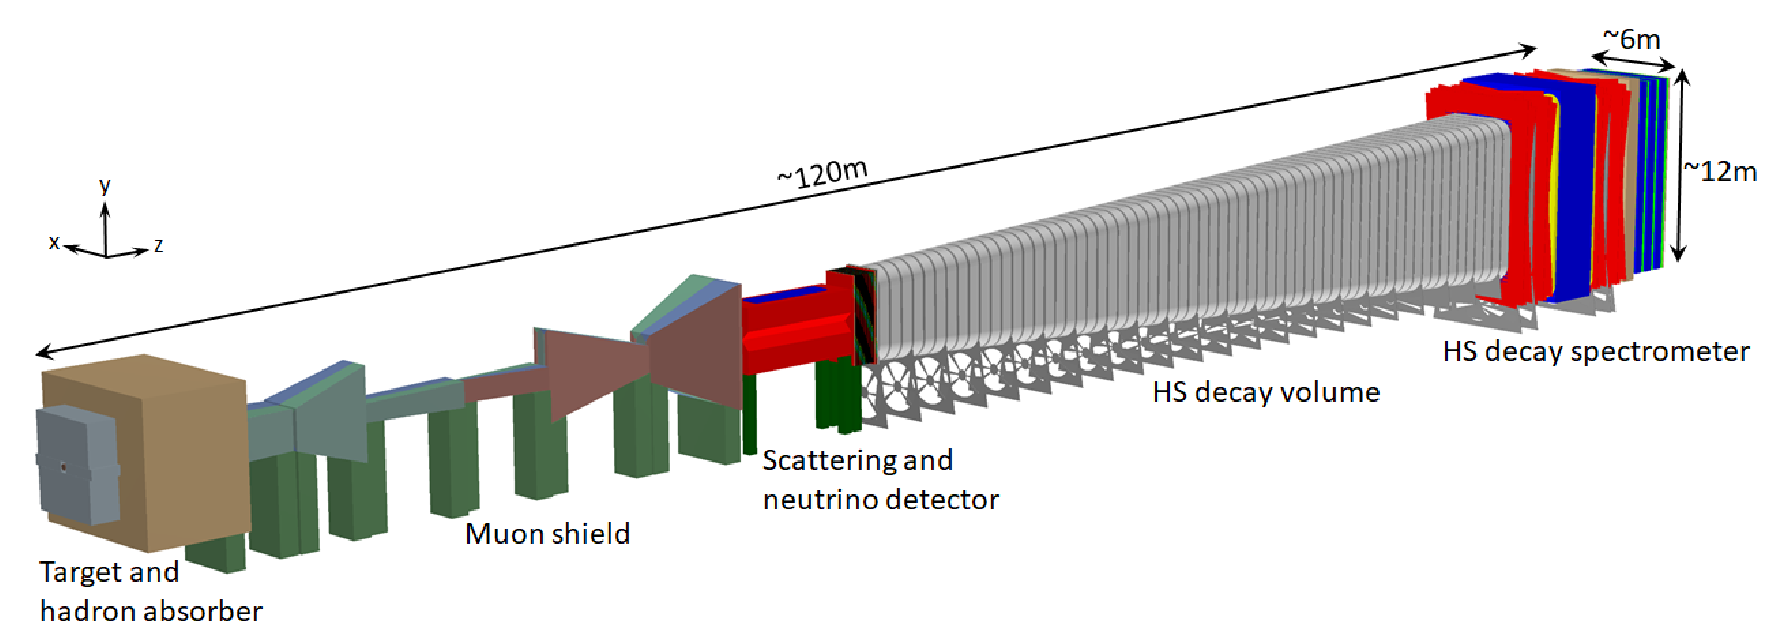
\includegraphics[width=1.\textwidth]{pictures/ship_sketch}
	\caption[Overview of the SHiP experiment.]{Overview of the proposed setup for the SHiP experiment. The target on the left is used as a beam dump for the SPS. Most \ac{sm} particles get absorbed by the hadron absorber directly behind the target. A magnetic muon shield deflects the muon, which will not be absorbed by the hadron absorber, away from the beam line. After the muon shield is a scattering and neutrino detector, and afterward, the \SI{50}{\meter} long decay volume in which non \ac{sm} particles created at the target can decay into \ac{sm} particles. Behind the decay volume, the decay spectrometer is placed. To achieve the zero background goal, the Surround Background Tagger is around the decay volume. \cite{ship_coll}}
	\label{fig:ship_sketch}
\end{figure}

One problem for the measurement is \ac{sm} particles entering the decay volume and getting falsely reconstructed as \ac{hs} events in the spectrometer.
An example of such a background is muons deflected by the muon shield and reflected at the walls of the facility into the decay volume, mimicking the decay products of an \ac{hs} event in the spectrometer.
Therefore it is crucial for the zero background requirement to detect the particles entering the decay volume and tag every event that could be caused by the entering particle as background.
This task is meant to be done by the \ac{sbt}.
As the name suggests, it surrounds the \ac{hs} decay volume, detecting particles entering it.
It is currently in development and this thesis is part of the R\&D effort toward it.
In the following, the \ac{sbt} and the principles of the different parts are described.
The details of the different parts important for this thesis are presented in more detail in the next chapter.

To make the tagging of background events possible and efficient and avoid the incorrect tagging of many \ac{hs} events different pieces of information need to be known about the particles entering the decay volume.
These pieces of information are the energy of the entering particles, the time at which they are entering the decay volume, and the space coordinates at which they are entering.
Therefore the \ac{sbt} is designed as a five-dimensional tagger.
It will consist of approximately 2000 cells that form the walls on the side as well as the top and bottom of the vacuum decay chamber.
The structure is shown in \autoref{fig:sbt}.
In order to fit the overall truncated pyramid shape of the decay volume, the cells have an unsymmetric shape, an example is shown in \autoref{fig:sbt}.
Both of the long edges are parallel, but the shorter sides are not.
The depth of the cells is \SI{20}{\centi\meter} and the wall thickness is planned to be \SI{2}{\centi\meter} \cite{}.
For the detection of particles, a liquid scintillator will be filled into the cells.
A particle passing through one or more cells will deposit energy in the scintillator, causing the emittance of scintillation light.
The amount of emitted light is correlated to the amount of energy deposited in the scintillator.
Two \acp{wom}, PMMA tubes coated with wavelengthshifting paint, are placed in each cell to collect the scintillation light and guide it to an array of \acp{sipm}.
The signals from the \acp{sipm} can be amplified, digitized, and further processed.
Both a \acp{wom} and a \ac{sipm} array are shown in \autoref{fig:sbt}.

\begin{figure}
	\centering
	\begin{subfigure}[b]{0.25\textwidth}
		\centering
		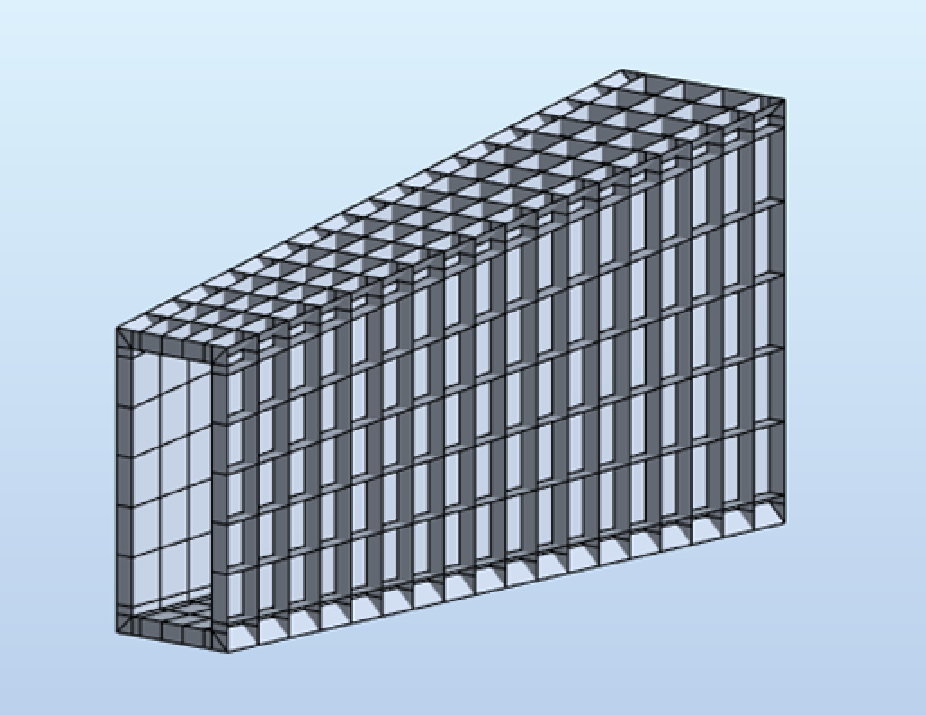
\includegraphics[width=.9\textwidth]{pictures/sbt_structure_sceleton}
		\caption{test}
		\label{fig:sbt_structure_sceleton}
	\end{subfigure}
	\begin{subfigure}[b]{0.25\textwidth}
		\centering
		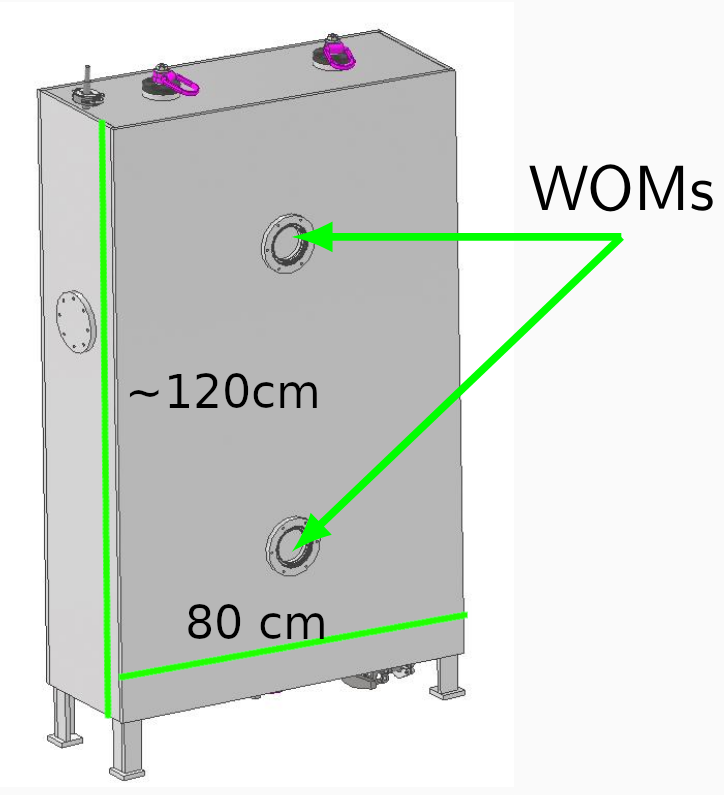
\includegraphics[width=.9\textwidth]{pictures/sbt_structure_cell}
		\caption{test}
		\label{fig:sbt_structure_cell}
	\end{subfigure}
	\begin{subfigure}[b]{0.25\textwidth}
		\centering
		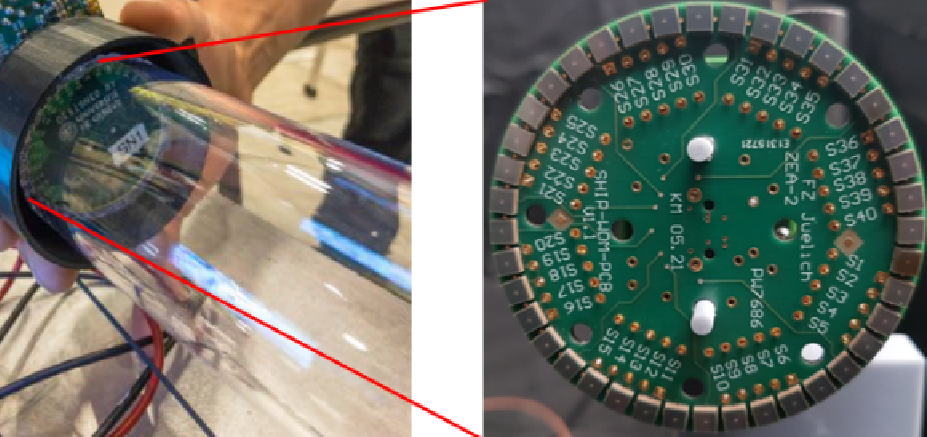
\includegraphics[width=.9\textwidth]{pictures/sbt_structure_wom}
		\label{fig:sbt_structure}
	\end{subfigure}
	\begin{subfigure}[b]{0.25\textwidth}
		\centering
		\includegraphics[width=.9\textwidth]{pictures/sbt_structure_sipm}
		\label{fig:sbt_structure}
	\end{subfigure}
	\caption[Overview of the Surrounding Background Tagger]{The structure of the Surrounding Background Tagger (SBT). Left is the SBT with its approximately 2000 cells. Then the shape of one example cell is shown in b). The light produced by the liquid scintillator inside the cells is captured by two Wavelengthshifting Optical Modules (WOMs) per cell, an example is shown in c), and then guided to an array of Silicon Photomultipliern, shown in d), which will detect the light.}
	\label{fig:sbt}
\end{figure}

This thesis is in the scope of the R\&D of the \ac{sbt}.
For the R\&D of the \ac{sbt}, a prototype of one of the cells was built, with which important parts can be tested.
Starting from the cell's material itself, a reflecting coating on the inside of the cell, the coated \acp{wom}, and the \acp{sipm} to name a few.
This thesis is about the readout of the \acp{wom} of the prototype.
Since the \ac{asic} meant to be used for the readout in the \ac{sbt} is in development by the Forschungszentrum Jülich and not yet finished, another readout is needed for the One Cell Prototype in order to test it.
The next chapter presents the One Cell Prototype with the focus on the \ac{wom} readout.

\chapter{One Cell Prototype}

The work presented in this thesis is done in the framework of the One Cell Prototype.
Therefore the prototype is described in more detail in this chapter.
Although the important parts of the One Cell Prototype are all mentioned here, the main focus lies on the amplifier and the digitizer since these are the most relevant parts of this thesis.
Firstly the cell and the liquid scintillator are shown, followed by the \ac{wom} used to capture the scintillation light, the \acp{sipm} used for the light detection, and the optical coupling between the \ac{wom} and the and the \acp{sipm}, are presented afterward.
Subsequently, the amplifier and the digitizer are introduced.



\section{The Cell \& Liquid Scintillator}

In \autoref{fig:one_cell}, the One Cell Prototype is shown.
It is \SI{80}{\centi\meter} wide and around \SI{120}{\centi\meter} high.
However, the precise height depends on the position in the cell due to the asymmetric shape.
The walls of the cell consist of \SI{1}{\centi\meter} thick corten steel.
The steel was chosen because of the rather low price tag, which is an important aspect considering the size of the \ac{sbt}.
A thickness of \SI{1}{\centi\meter} is only half of the planned \SI{2}{\centi\meter} wall thickness of the \ac{sbt} design.
The \ac{sbt} needs such thick walls in order to withstand the vacuum on the inside.
For the R\&D with the One Cell Prototype, the thickness was reduced to be able to perform measurements with different wall thicknesses by adding steel plates to the outside.
This is important in case the \ac{sbt} design changes, for example by replacing the vacuum with helium.
One side of the cell has two holes with a \SI{}{\centi\meter} radius.
They have an equal distance to both side walls.
The lower hole is \SI{30}{\centi\meter} away from the bottom of the cell, and the upper hole is \SI{30}{\centi\meter} below the top.
In each of these holes, a PMMA vessel, shown in \autoref{fig:pmma_vessel}, is placed to house the two \acp{wom} and protect their wavelengthshifting coating from the liquid scintillator.
A reflective paint was applied to the inside of the cell to increase the scintillator's light yield and therefore increase the detector's efficiency.
\begin{figure}
	\centering
	\begin{subfigure}[b]{.40\textwidth}
		\centering
		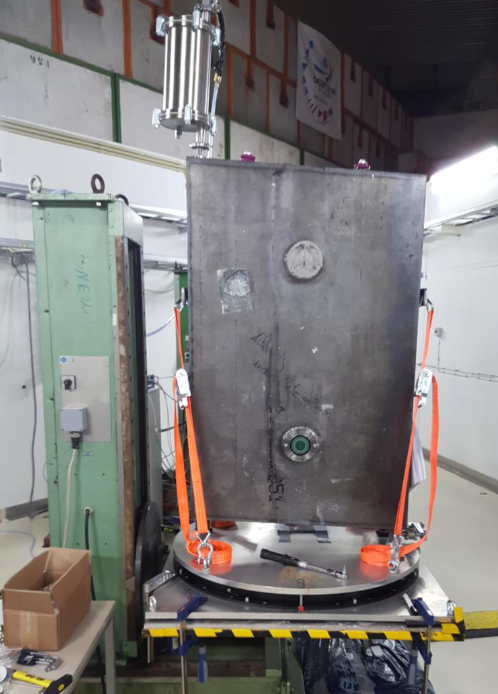
\includegraphics[width=1.\textwidth]{pictures/one_cell}
		\caption[One Cell Prototype]{}
		\label{fig:one_cell}
	\end{subfigure}
	\begin{subfigure}[b]{.54\textwidth}
		\centering
		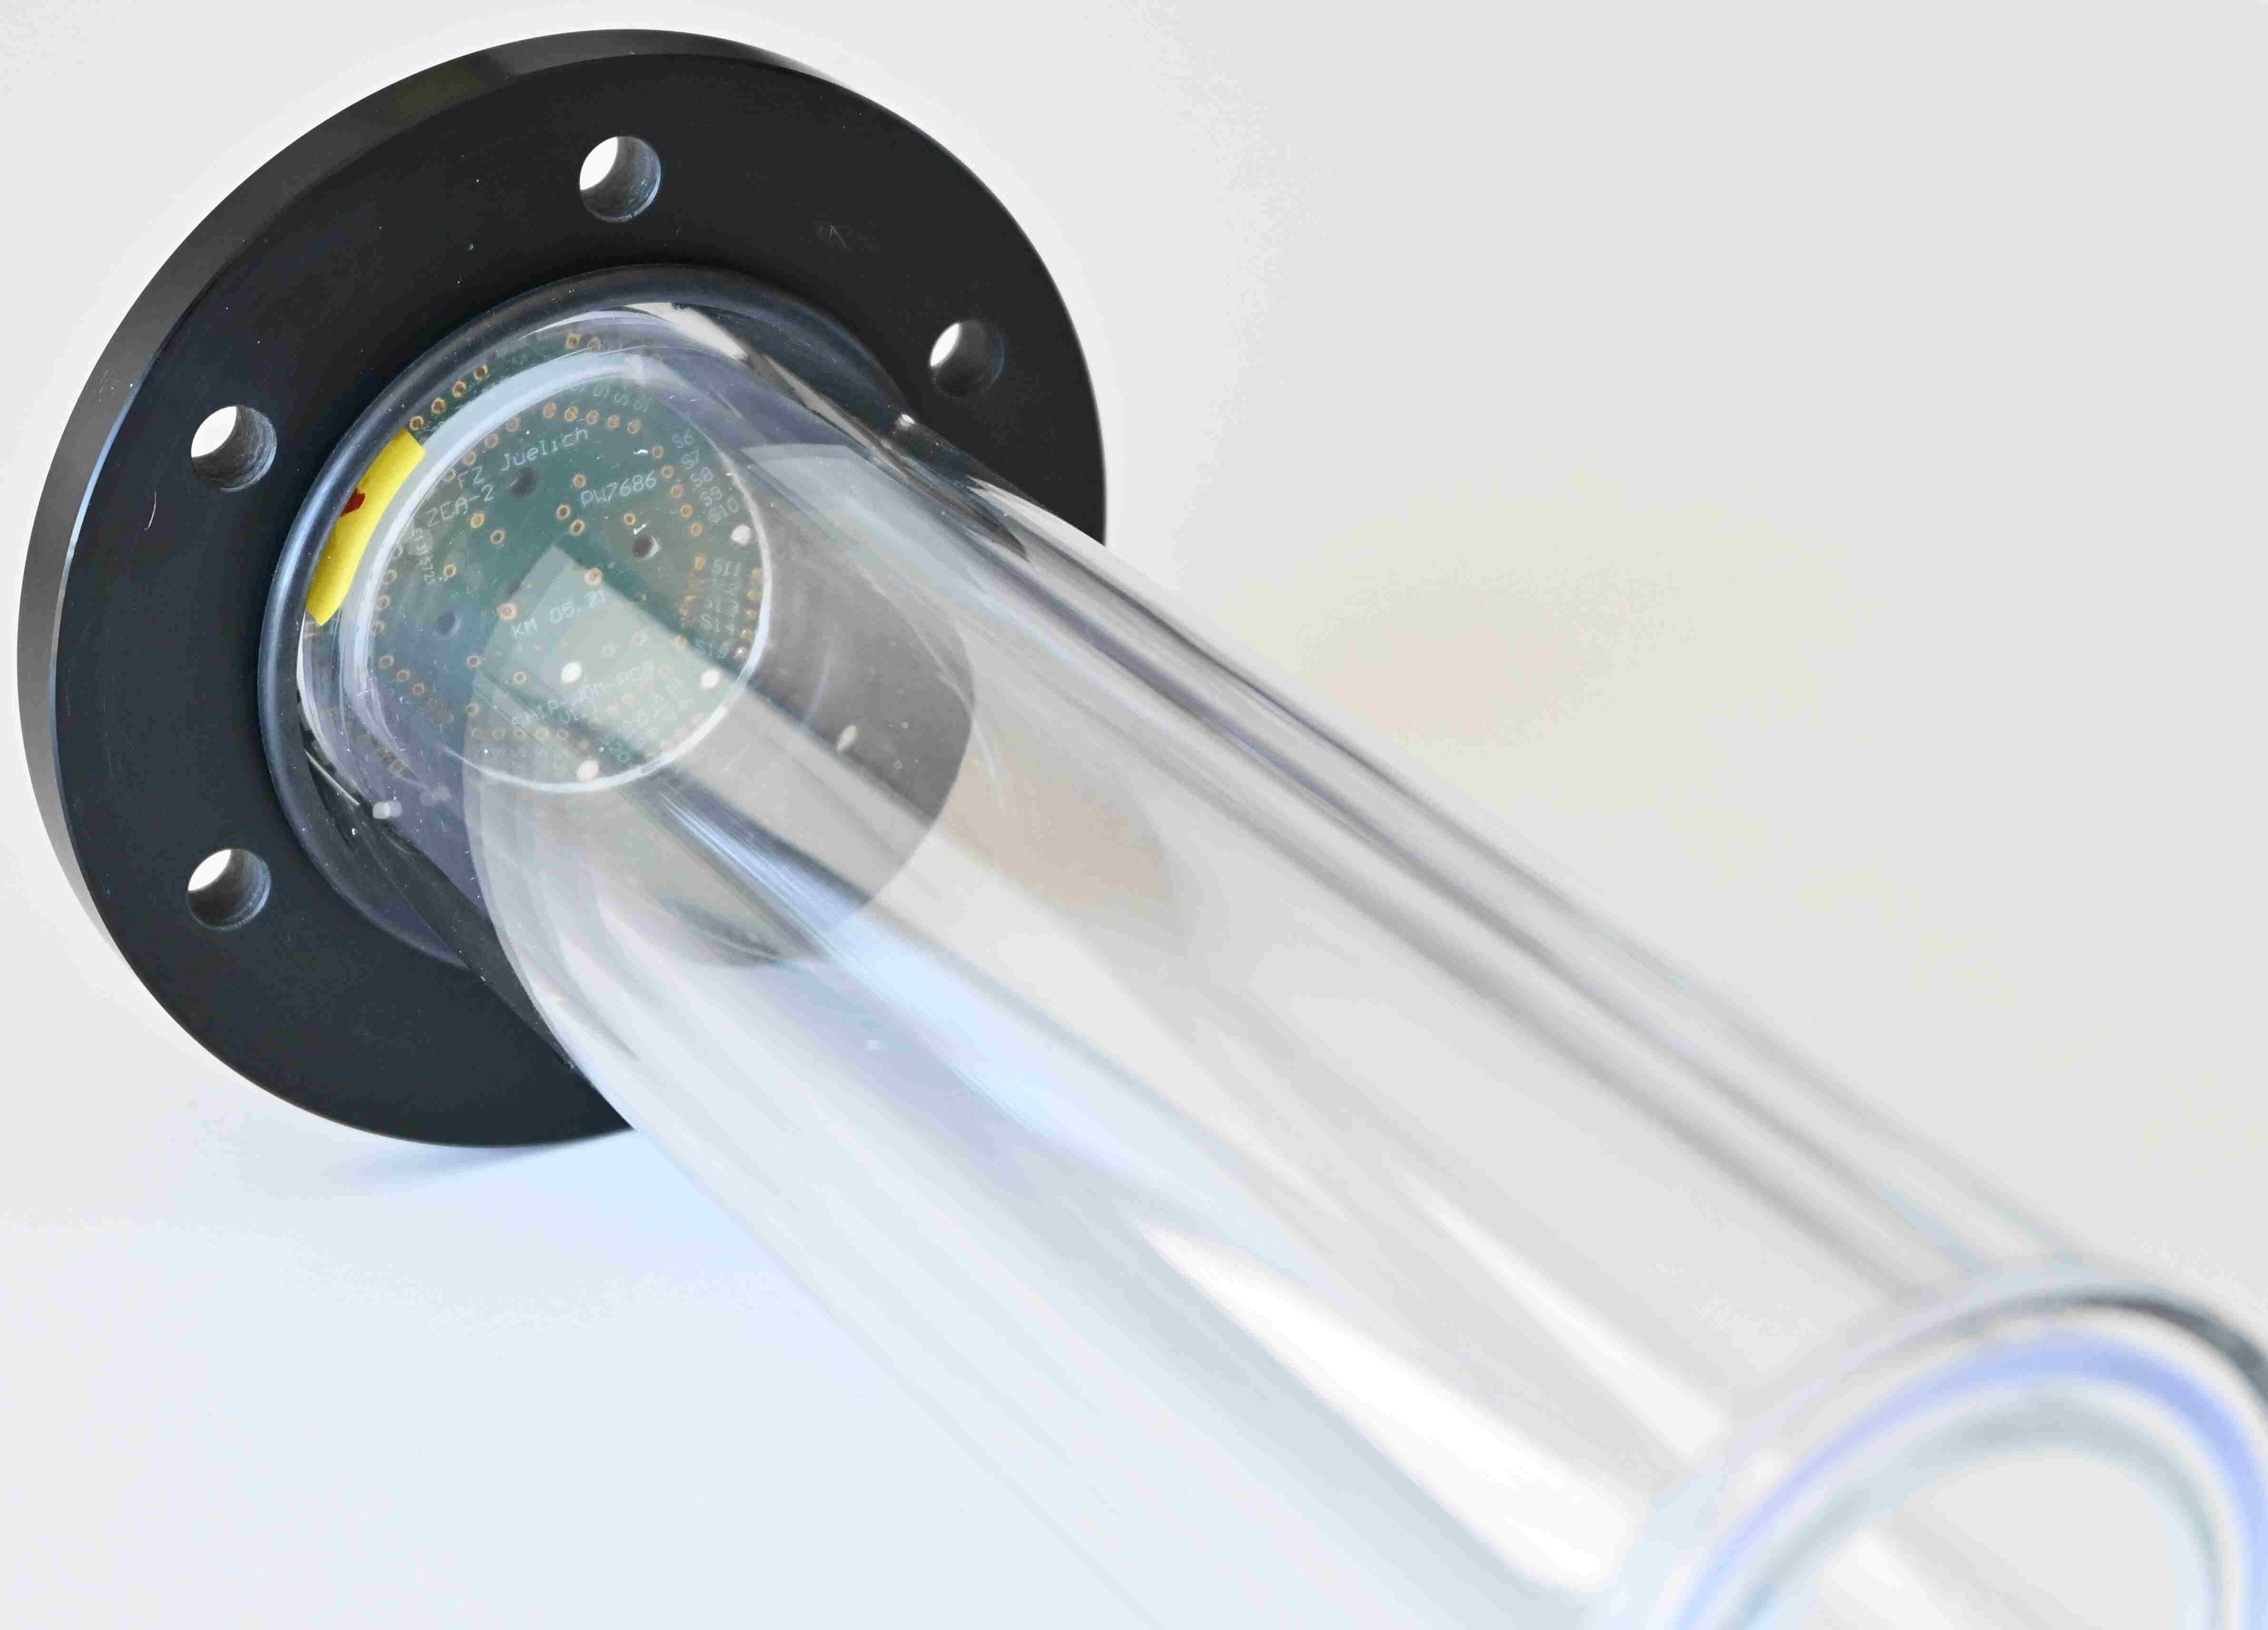
\includegraphics[width=1.\textwidth]{pictures/pmma_vessel}
		\caption[PMMA vessel]{}
		\label{fig:pmma_vessel}
	\end{subfigure}
	\caption[One Cell Prototype and PMMA vessel]{The One Cell Prototype at the DESY testbeam area a) and a PMMA vessel with a Wavelenthshifting Optical Module inserted and a \ac{sipm} board attached b). \cite{}}
	\label{fig:one_cell_and_pmma}
\end{figure}

The cell is filled with the liquid scintillator \ac{lab} mixed with \SI{2}{\gram\per\liter} Diphenyloxazole (PPO)%, which is also planed to be used in the \ac{sbt}.
In order to allow decrompression and compression by temperature change, an expansion vessel is mounted on top of the cell.
%To fill the cell \SI{}{\kilo\gram} \ac{lab} were used.
%This is around \SI{3}{\kilo\gram} more than the amount fitting into the cell.
%The extra \ac{lab} is in the expansion vessel, in order for the cell still being full in case of a temperatur decline and compession of the \ac{lab}.
The cell was overfilled with scintillator, in order to still being full if the temperature declines and the scintillator compresses.
Gaseous nitrogen fills out the remaining volume of the expansion vessel to serve as a compressible volume. 

\ac{lab}s emission spectrum is shown in \autoref{fig:lab_emission}.
Most of the scintillation light has a wavelength of \SIrange{320}{360}{\nano\meter}.
In order to capture the light and to shift the wavelength towards values for which the used \acp{sipm} have a higher detection efficiency, \acp{wom} are used.
In the next section, these \acp{wom} and the optical coupling between them and the \acp{sipm} are presented.
\begin{figure}
	\centering
	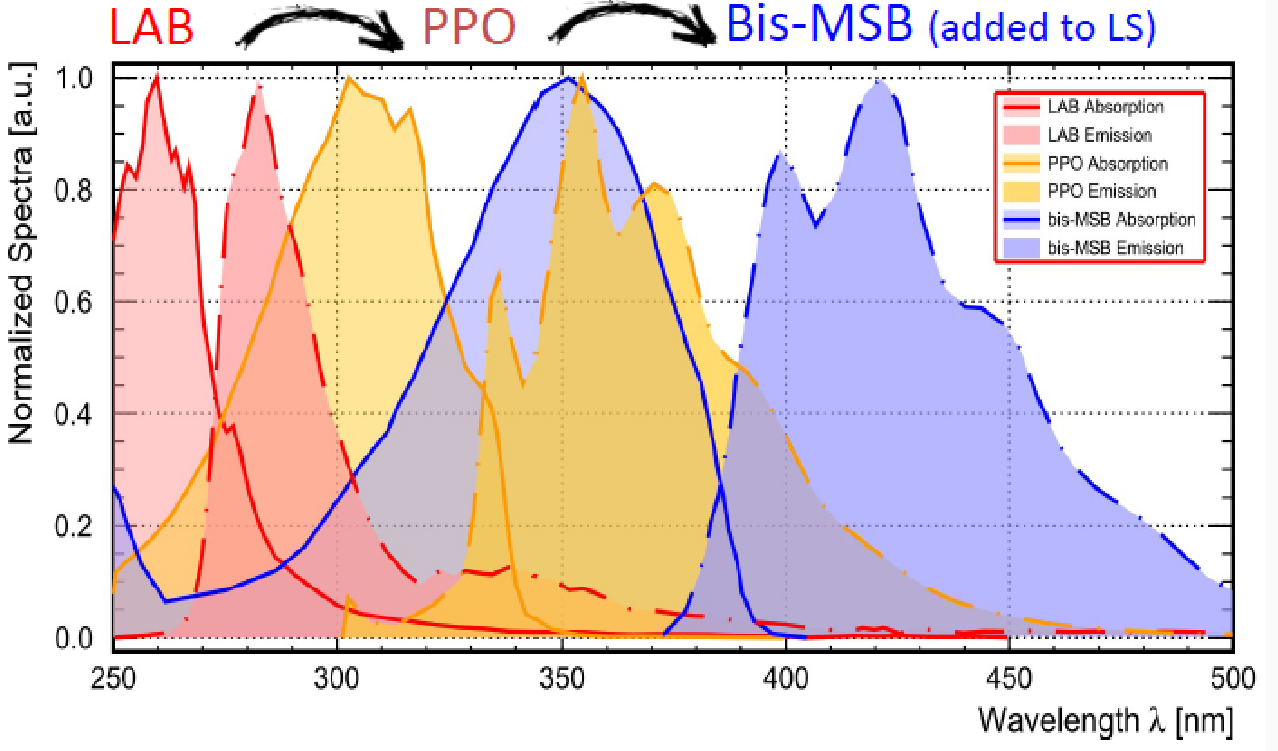
\includegraphics[width=.8\textwidth]{pictures/lab_emission}
	\caption[LAB emission spectrum]{The emission spectrum of the liquid scintillator components \ac{lab} and \ac{ppo} and the wavelength shifter Bis-MSB. \cite{}}
	\label{fig:lab_emission}
\end{figure}



\section{Wavelengthshifting Optical Module \& Optical Coupling}

So-called \acp{wom} are used to capture the scintillation light.
They are PMMA cylinder walls with a \SI{6}{\centi\meter} outer diameter and a \SI{3}{\milli\meter} wall thickness.
The design and material choice both make the cost of the light collection relatively cheap.
Both the inside and outside of the PMMA cylinder are coated with the wavelength shifter Bis-MSB \cite{}.
So the captured photons are shifted to a higher wavelength, for which the \acp{sipm} used for the light detection have a higher efficiency.
\autoref{fig:lab_emission} shows the wavelength spectrum of the wavelength-shifted light.
The photons which enter the \ac{wom} are trapped there by total reflection on the walls.
They can leave the \ac{wom} at its end, where an array of forty \acp{sipm} can detect them.
For a good optical coupling between the \ac{wom} and the \acp{sipm}, either optical grease or silicon pads can be used.
\autoref{fig:wom_principle} illustrates the principle of the \ac{wom} with the wavelength shifting and capture by total reflection.
\begin{figure}
	\centering
	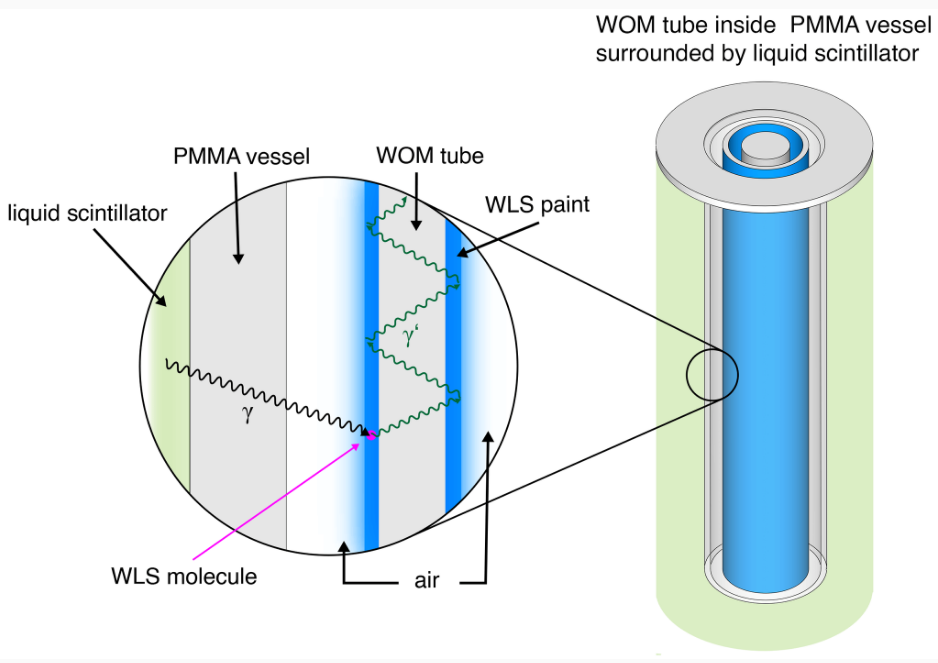
\includegraphics[width=.8\textwidth]{pictures/wom_principle}
	\caption[Working principle of a WOM]{A Wavelengthshifting Optical Module (WOM) is a PMMA tube coated with the wavelength shifter Bis-MSB. If a photon in the UV range hits the WOM, its wavelength gets shifted. Afterward, in the WOM, the photon is trapped by total reflection. At the end of the WOM, the photon can be detected by a photosensor. \cite[]}
	\label{fig:wom_principle}
\end{figure}

In the next part, the \acp{sipm}, which detect the light captured by the \acp{wom}, are presented.


\section{Silicon Photomultiplier}
In order to correctly identify and tag background events, the light detection of the \ac{sbt} has to provide accurate timing information.
Furthermore, due to the number of cells and \acp{wom} in the \ac{sbt}, it should not cost a lot per \ac{wom}.
To fulfill both requirements, \acp{sipm} were chosen as photodetectors.
These photodetectors consist of up to thousands of pixels.
Each pixel is a photodiode with a typical edge length between \SI{10}{\micro\meter} and \SI{100}{\micro\meter} \cite{nucl}.
If triggered by light, a \ac{sipm} sends out a charge signal proportional to the number of triggered pixels.
In the case that the number of incoming photons is low compared to the number of pixels, such that two photons hitting the same pixel is unlikely, the charge signal is linear to the light intensity.
The charge signal possesses a fast-rising edge with a rise time of the order of tens of \si{\piko\second} \cite{nucl}.
Besides the excellent time resolution, \acp{sipm} also make it possible to count the arriving photos with a sensitivity down to single photons \cite{HAMA_mppc}.

Each pixel in the \ac{sipm} is an \ac{spad}, which is a \ac{apd} supplied with a voltage greater than its breakdown voltage.
In the following, the principle of such an \ac{apd} and \ac{spad} are explained.

Similar to every photodiode, \ac{apd} utilize, the photoelectric effect to generate an electric charge signal in response to a light signal.
They consist of doped silicon.
An example is shown in \autoref{fig:pin_diode}.
It has a strongly n-doped layer, followed by a strongly p-doped layer, an intrinsic, weakly p-doped layer, and another p-doped layer.
By adding the intrinsic layer, the region in which the photons can be absorbed increases.
If a photon gets absorbed, it generates an electron-hole pair.
When a reversed bias voltage is applied, the electric field in the \ac{apd} separates the $eh$-pair.
In case the \ac{apd} is operated in the Geiger mode, meaning the bias voltage is higher than the breakdown voltage of the \ac{apd}, the electric field at the strongly doped $p$- and $n$-layer is sufficiently high, that a self-sustaining avalanche is triggered by either the electron or the hole moving through it.
Then the \ac{apd} is called \ac{spad}.
The macroscopic signal of a \ac{spad} makes it possible to detect single photons.
In order to stop the avalanche, a quenching resistor is connected in series to the \ac{spad}.
With an increasing current signal flowing through the quenching resistor, the voltage drop at this resistor increases, and thus the bias voltage at the \ac{spad} decreases.
When the bias voltage drops under the breakdown voltage, the avalanche is no longer self-sustaining and stops.
Thus the signal amplitude of a \ac{spad} is always similar, independent of how many photons arrive at the same moment.


%Similar to every photodiode, \acp{apd} utilize the photoelectric effect, to generate an electric charge signal in response to a light signal.
%This is made possible by using silicon as a base material and introducing impurities. 
%This process is called doping and there are two different possibilities for doping. 
%In the n-doping, the impurities are atoms with five valence electrons.
%Four of these electrons are part of boundings with silicon atoms, and the fifth electron is only weakly bound.
%When p-doping, atoms with only three valence electrons are inserted into the silicon.
%This leads to missing charges in the silicon, called holes.
%By having an n-doped and a p-doped region in the silicon, the excess electrons from the n-doped region combine with the holes from the p-doped region, resulting in a depleted region at the pn-junction.
%If a photon hits the photodiode, it can create an electron-hole pair, or $eh$-pair.
%The electron and the hole get split by the electric field and thus create a charge signal.
%In order to increase the sensitivity of the photodiode, an intrinsic layer can be added in between the two doped regions, thus increasing the depletion layer and therefore the photosensitive area.
%Such a photodiode is called a pin-diode.
%An \ac{apd} with a weakly doped $\pi$ intrinsic layer and strongly doped $p^+$ and $n^+$ layers is shown in \autoref{fig:pin_diode}.
%This intrinsic layer can either be not doped at all or weakly doped.
%In the case of \acp{apd} the intrinsic layer is weakly doped. 
%In order to amplify the signal, a strong doped region is inserted, thus creating a multiplication zone.
\begin{figure}
	\centering
	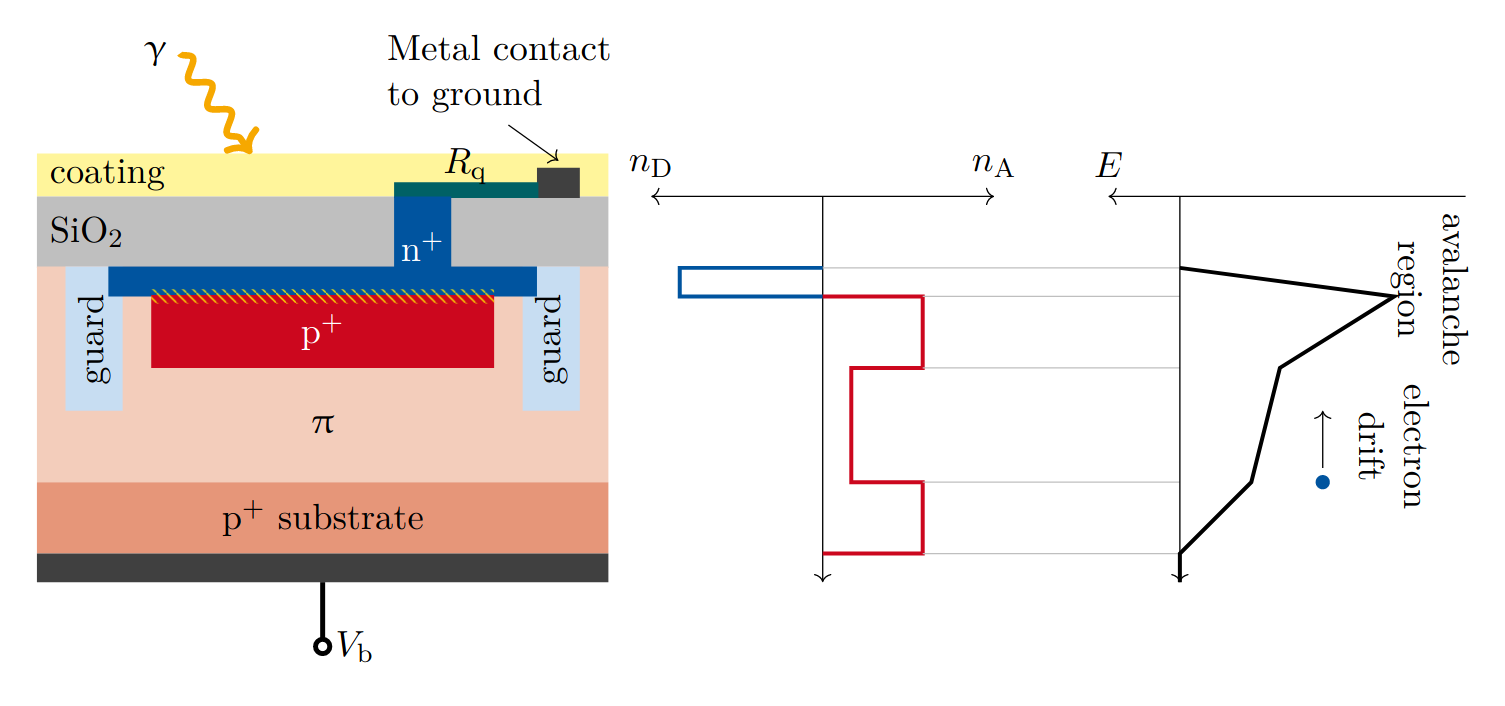
\includegraphics[width=1.\textwidth]{pictures/pin_diode}
	\caption[Illustration of a APD.]{Composition of an avalanche photodiode with the bias voltage $V_\text{B}$ applied in the reverse direction. Between the contact to the ground and the strongly doped $n^+$ layer is the quenching resistor $R_\text{q}$ connected in series. Next to the $n^+$ layer is a strongly doped $p^+$ layer. In the region of these two layers is the electric field, shown in the right figure, the strongest. There, an electron or hole can initiate an avalanche. After the $p^+$ layer is an intrinsic weakly doped $\pi$ layer. This layer increases the sensitive volume of the diode. If a electron-hole pair is created, it gets separated by the electric field. The hole drifts towards the multiplication region and can start an avalanche. The next layer is a $p^+$ layer, which connects to a metal connector and high voltage. The picture in the middle illustrates the number of donators $n_D$ ad acceptors $n_A$, and the last picture illustrates the field strength at the different regions of the \ac{apd}. \cite{}}
	\label{fig:pin_diode}
\end{figure}

%When a reverse bias voltage is applied to the \ac{apd}, the electric field between the $n^+$ and $p^+$ layers is strong enough that a created $eh$-pair creates more $eh$-pairs, resulting in an avalanche.
%For this avalanche process to be possible the reverse bias voltage must be at or above the breakdown voltage of the \ac{apd}.
%With such a bias voltage applied, the \ac{apd} operates in the Geiger mode and the avalanche is then self-sustaining.
%This results in a macroscopic signal and makes the detection of single photons possible.
%Therefore these diodes are also called \ac{spad}.
%To stop the avalanche, a quenching resistor is connected in series with the \ac{spad}.
%With an increasing current signal flowing through the quenching resistor, the voltage drop at this resistor increases, and thus the bias voltage at the \ac{spad} decreases.
%When the bias voltage drops under the breakdown voltage, the avalanche is no longer self-sustaining and stops.
%Thus the signal amplitude of a \ac{spad} is always similar, independent of how many photons arrive at the same moment.

In \acp{sipm}, hundreds to thousands of \acp{spad} are connected in parallel, each with a high-resistance quenching resistor in series. 
Usually, the \ac{spad} pixels are placed in a rectangular form with an edge length of a few \si{\milli\meter}.
\autoref{fig:sipm_closeup} shows a picture of a \ac{sipm} and one picture of a single pixel of a \ac{sipm}.
Due to the property of the \acp{spad} that the output signal is always similar for each \ac{spad}, the output signal of a \ac{sipm} is the output signal of one \ac{spad} multiplicated by the number of triggered \acp{spad}.
Therefore, if the number of photons arriving simultaneously at a \ac{sipm} is low enough that the probability of one \ac{spad} being hit by two or more photons is low, one can count photons with a \ac{sipm}.
This and the relatively low cost, high durability, and impassivity to magnetic fields make them a good option for photodetection for the \ac{sbt} and similar detectors.
However, due to the sensitivity down to single photons, also $eh$-pairs created by thermal excitation will cause signals indistinguishable from signals caused by photons.
These signals are called \ac{dc}.



%In the following different properties of \acp{sipm} are presented, beginning with the signal shape of a single \ac{spad} and of a \ac{sipm}.


%\paragraph{The signal shape} of a \acp{spad} starts with a fast exponential rise with the time constant 
%\begin{align}
%	\tau_\text{rise}&=R_\text{S}\cdot C_\text{d}
%\end{align}
%with the resistance $R_\text{rise}$ and capacitance $C_\text{d}$ of the \ac{spad} \cite{HAMA_mppc}.
%After the signal reached its maximum current at around 
%\begin{align}
%	I_\text{max}&\approx \frac{V_\text{ov}}{R_\text{q}}
%\end{align}
%the quenching and recharging of the \ac{spad} starts.
%Thus the current signal decreases again exponentially.
%The time constant for the signal decay
%\begin{align}
%	\tau_\text{decay} &= R_\text{q}\cdot C_\text{d}
%\end{align}
%depends on the capacitance $C_\text{d}$ of the \ac{spad} and the quenching resistor $R_\text{q}$ \cite{HAMA_mppc}.
%This signal develpment is shown in \autoref{fig:spad_signal_shape}.
%\begin{figure}
%	\centering
%	\includegraphics[width=0.75\textwidth]{pictures/spad_signal_shape}
%	\caption[SPAD signal shape]{Single photon avalanche diode signal shape. The exponential rise with the time constant $R_\text{S}\cdot C_\text{d}$ is followed by the exponential decay with the time constants $R_\text{q}\cdot C_\text{d}$. The maximum of the current signal is at approximately $V_\text{ov}/R_\text{q}$ \cite{HAMA_mppc}}
%	\label{fig:spad_signal_shape}
%\end{figure}

%When multiple \acp{spad} in a \ac{sipm} are triggered, the output signal will be the summation of the signals from all triggered \acp{spad}.
%Besides the number of triggered \acp{spad}, the time difference between the signals from the single \acp{spad} influences the signal.
%In the case, that all \acp{spad} are triggered at the same time, the \ac{sipm} signal will have the shape of a \ac{spad} signal scaled up by the factor of the number of triggered \acp{spad}.
%If the signals form the individual \acp{spad} have a small difference in time, the \ac{sipm} signal will become broader.



An essential property of a \ac{sipm} is the gain $G$.
It describes the number of charge carriers released in each avalanche.
Due to the quenching, this parameter is well-defined \cite{}.
It can be calculated from the applied voltage $U_\text{bias}$, the breakdown voltage $U_\text{bd}$ and the capacitance $C_\text{d}$ of a \ac{spad} with
\begin{align}
	G &= \frac{(V_\text{bias}- V_\text{bd})\cdot C_\text{d}}{\text{e}}.
\end{align}
Here, e represents the charge of one electron.
Usually, the gain is in the order of $10^5$ to $10^7$ \cite{nucl}.
Since the breakdown voltage of different \acp{sipm} of the same model can differ slightly, also the gain with the same bias voltage can differ.

The next section presents the \ac{asic} used to amplify the \ac{sipm} signals.
%\paragraph{The noise} in \acp{sipm} can be sorted into two categories.
%The first is primary noise, it describes the triggering of avalanches by thermaly created $eh$-pairs and not by incident photons.
%Because the rate of theses thermaly caused events increases and decreases with the temperature, by controling the temperatur one can influence and decrease the rate of primary noise events.
%The second category is the correlated noise.
%It includes all events triggered by a primary event.
%This correlated noise does have two causes.
%One cause is the trapping and releasing of charge carriers from the avalanche. 
%When the time between the trapping and releasing is long enough, the avalanche of the primary event stoped and the released carrier can trigger another avalanche.


\section{The eMUSIC board}
Since the signals of the \acp{sipm} are tiny, they need to be amplified.
For this purpose, the \ac{emusic} \ac{asic} by Scientifica was chosen, and a custom \ac{pcb} housing the \ac{emusic} \ac{asic}, from here on called \ac{emusic} board, was designed by the electrical engineers of the University of Freiburg.
In the following first, the \ac{asic} itself and afterward, the \ac{emusic} board will be presented.

\paragraph{The eMUSIC ASIC} was developed by Scientifica for the readout of \acp{sipm}.
It is mainly an amplifier and a shaper, but it also offers other options like digital trigger signals if the signal crosses an adjustable threshold.
The \ac{asic}\'s block diagram is shown in \autoref{fig:emusic_block_diagram}.
\begin{figure}
	\centering
	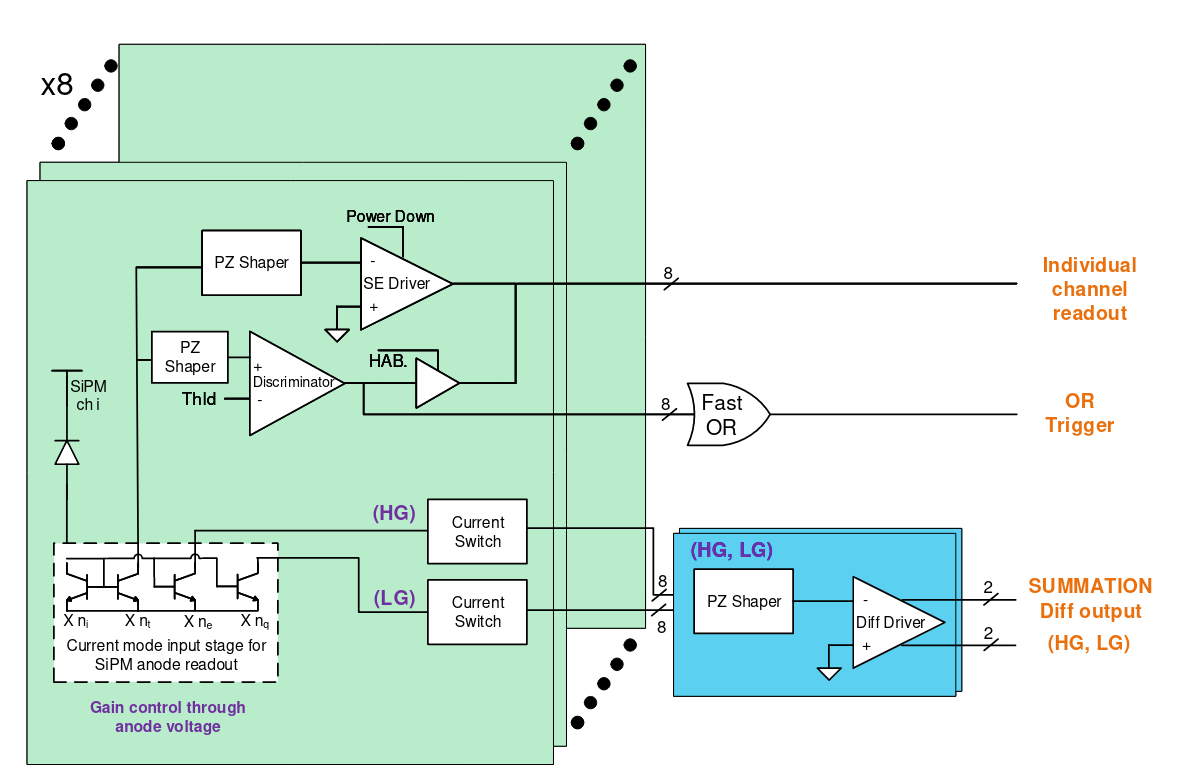
\includegraphics[width=1.\textwidth]{pictures/emusic_block_diagram.png}
	\caption[eMUSIC block diagram]{The block diagram of the \ac{emusic} \ac{asic}. At the input is the current mode input stage, which can also set an offset voltage on the input to adjust the overvoltage channel by channel. The signal then gets shaped by the pole-zero cancellation shaper and amplified and can be read out for each channel as a single-ended signal. The discriminator can set a threshold to create a digital signal which can be read out channel by channel instead of the analog output signal. A fast OR output can also be used to put out a digital OR of all eight discriminator outputs. With the summation outputs, one can put out the sum of an arbitrary set of channels with two gains as differential signals. \cite{gomez}}
	\label{fig:emusic_block_diagram}
\end{figure}
It has eight input channels, each equipped with a $\approx\SI{1}{\volt}$ anode voltage control to equalize the applied overvoltage between the different channels.
Because the \acp{sipm} deliver a charge signal, each channel has a current mode input stage.
The \ac{emusic} \ac{asic} was designed to have a low input transimpedance but provides the option of a high transimpedance mode with which the gain can be increased.
Each individual channel has a bandwidth of \SI{150}{\mega\hertz} and a pole-zero cancellation, schematics shown in \autoref{fig:emusic_pole_zero}, with two adjustable resistors and an adjustable capacitor.
It can be used to decrease the \ac{fwhm} of the output signal to below $\SI{10}{\nano\second}$.
But a smaller width also attenuates the amplitude of the signal.
The resistor has eight possible values it can be set to, and the capacitor has thirty-two different steps.
Although the \ac{emusic} provides the option of a lower attenuation mode of the pole-zero cancellation, a compromise between smaller signal width and higher amplitude should be chosen depending on one's needs.
Alternatively, the pole-zero cancellation can be disabled completely, resulting in the highest signal amplitude possible with the \ac{emusic} but also in the longest signal.
The signal after the shaper can be put out with an analog output for each channel.
\begin{figure}
	\centering
	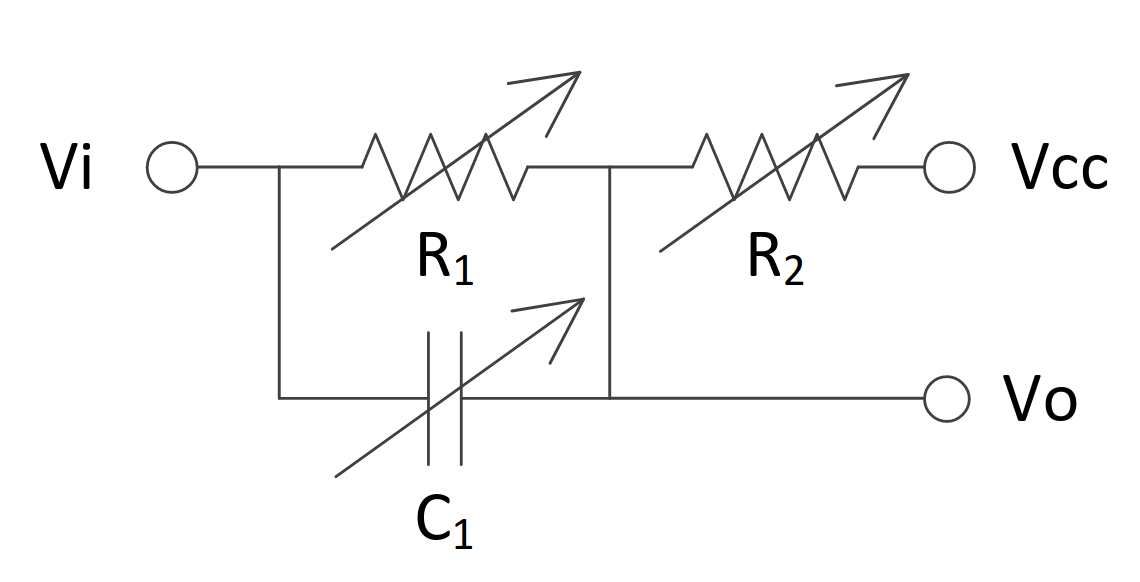
\includegraphics[width=0.5\textwidth]{pictures/emusic_pole_zero.png}
	\caption[eMUSIC pole-zero cancellation]{Sketch of a pole-zero cancellation with adjustable resistors and capacitor, the input voltage $\text{V}_\text{i}$, the output voltage $\text{V}_\text{o}$, and the operation voltage $\text{V}_\text{cc}$. \cite{gomez}}
	\label{fig:emusic_pole_zero}
\end{figure}

Each channel also possesses a discriminator with an adjustable threshold to create a channel-by-channel trigger signal.
These logical signals can be either put out by using the individual output of the channel for the digital signal instead of the analog waveform or by using the fast OR of all channels.
This fast OR allows, for example, the external triggering of the digitizer, which then digitizes the analog waveforms if the waveform of one or more channels surpasses the threshold.
The dynamic range of the output for the single-ended signals is \SI{1}{\volt} if the load on the output is \SI{50}{\ohm} and \SI{2}{\volt} if a high impedance load is used on the output.
Using the low transimpedance mode, the gain of the single-ended output is \SI{180}{\ohm}, and with the high transimpedance mode, it is \SI{480}{\ohm}.
Over the first half of the dynamic range, the response of the \ac{emusic} is linear, and over the second half, it is non-linear.

Besides the individual readout of the eight channels, the \ac{emusic} can sum up the signal of an arbitrary set of channels with both high and low gain and put them out via two differential outputs.
The bandwidth of this summation output is \SI{500}{\mega\hertz}, and the output range is \SI{1.25}{\volt}.
Depending on whether the high or low transimpedance is used, the gain of the high gain summation is \SI{690}{\ohm} or \SI{90}{\ohm} and \SI{315}{\ohm} or \SI{45}{\ohm} for the low gain summation. 
The response of the summation output is linear over the dynamic range.

Besides choosing the channels for summation, also each of the eight single-ended outputs can be individually turned on and off.
Another important option that can be configured is the adjustment of the output DC offset to maximize the rail-to-rail voltage swing.

\paragraphe{The trigger threshold} for the digital outputs can be set with two parameters.
The first one is the bandgap voltage $V_\text{bg}$ of the comparators, which can be adjusted in eight steps between \SI{487.22}{\milli\volt} and \SI{2436.8}{\milli\volt}.
The second parameter sets the \ac{dac} value $N_\text{DAC}$ for the comparators.
It can be set to \ac{dac} counts from 0 to 511.
The finer threshold steps $V_\text{fine}$ can be calculated with
\begin{align}
	V_\text{fine}&=\SI{1637.79}{\milli\volt} - N_\text{DAC}\cdot\SI{3.1445}{\milli\volt}.
\end{align}
With $V_\text{bg}$ and  of $V_\text{fine}$ or $N_\text{DAC}$, the final threshold
\begin{align}
	V_\text{th}&= 1.5\cdot V_\text{bg} - 0.5\cdot V_\text{fine}\\
		   &= 1.5\cdot V_\text{bg} - 0.5\cdot (\SI{1637.79}{\milli\volt} - N_\text{DAC}\cdot\SI{3.1445}{\milli\volt})
\end{align}
can be calculated.

\paragraph{The eMUSIC board} was designed at the University of Freiburg.
A graphic of the board is shown in \autoref{fig:emusic_board}.
Its heart is the \ac{emusic} \ac{asic} (U1).
In order to program the \ac{asic}, the ATmega328P-AU microchip (U4) is placed on the board.
The microchip can be programmed with the XXXX software by XXXXX and the XXXXX, which is connected to the computer via USB and can be plugged into the J4 connector on the \ac{emusic} board.
After programming the microchip, it only has to be programmed again if the reset button SW1 is pressed.
Then the \ac{emusic} \ac{asic} can be configured by using a TTL-to-USB adapter connected to a computer and the P3 connector, and the software of the minimusic board.
The minimusic board is a commercial product using the \ac{emusic} \ac{asic}.
Due to the \ac{emusic} board being designed to work with the minimusic software, one avoids the need to write software and also has the security that the used software was tested and is working correctly.
Two functions of the minimusic software are not usable on the \ac{emusic} board, the calibration of the threshold and the calibration of the DC offset on the outputs.
Therefore these two need to be set by the user.

The high voltage for the \acp{sipm} can be supplied via the P2 SMA connector.
On the backside of the \ac{pcb} is an LSHM-150-XX.-XXX-DV-AN-XX connector located to connect the board to the \ac{sipm} board.
Via this connector, the high voltage is brought to the \acp{sipm}, and the signals are brought to the \ac{emusic} inputs.
The eight single-ended outputs can be read out by the SMA connectors K1 to K8.
The fast OR signal can be read out via the K9 connector.
Both the high and low gain differential summation outputs are connected to the pins of the J6 connector.

The board also provides the possibility via the P1 connector to power the six LEDs soldered onto the \ac{sipm} boards.
However, the usage of this is not advised since this will introduce interferences into the signals.

The amplified single-ended output signals then can be digitized.
For this task, the GANDALF module was chosen, which is described in the next section.

\begin{figure}
	\centering
	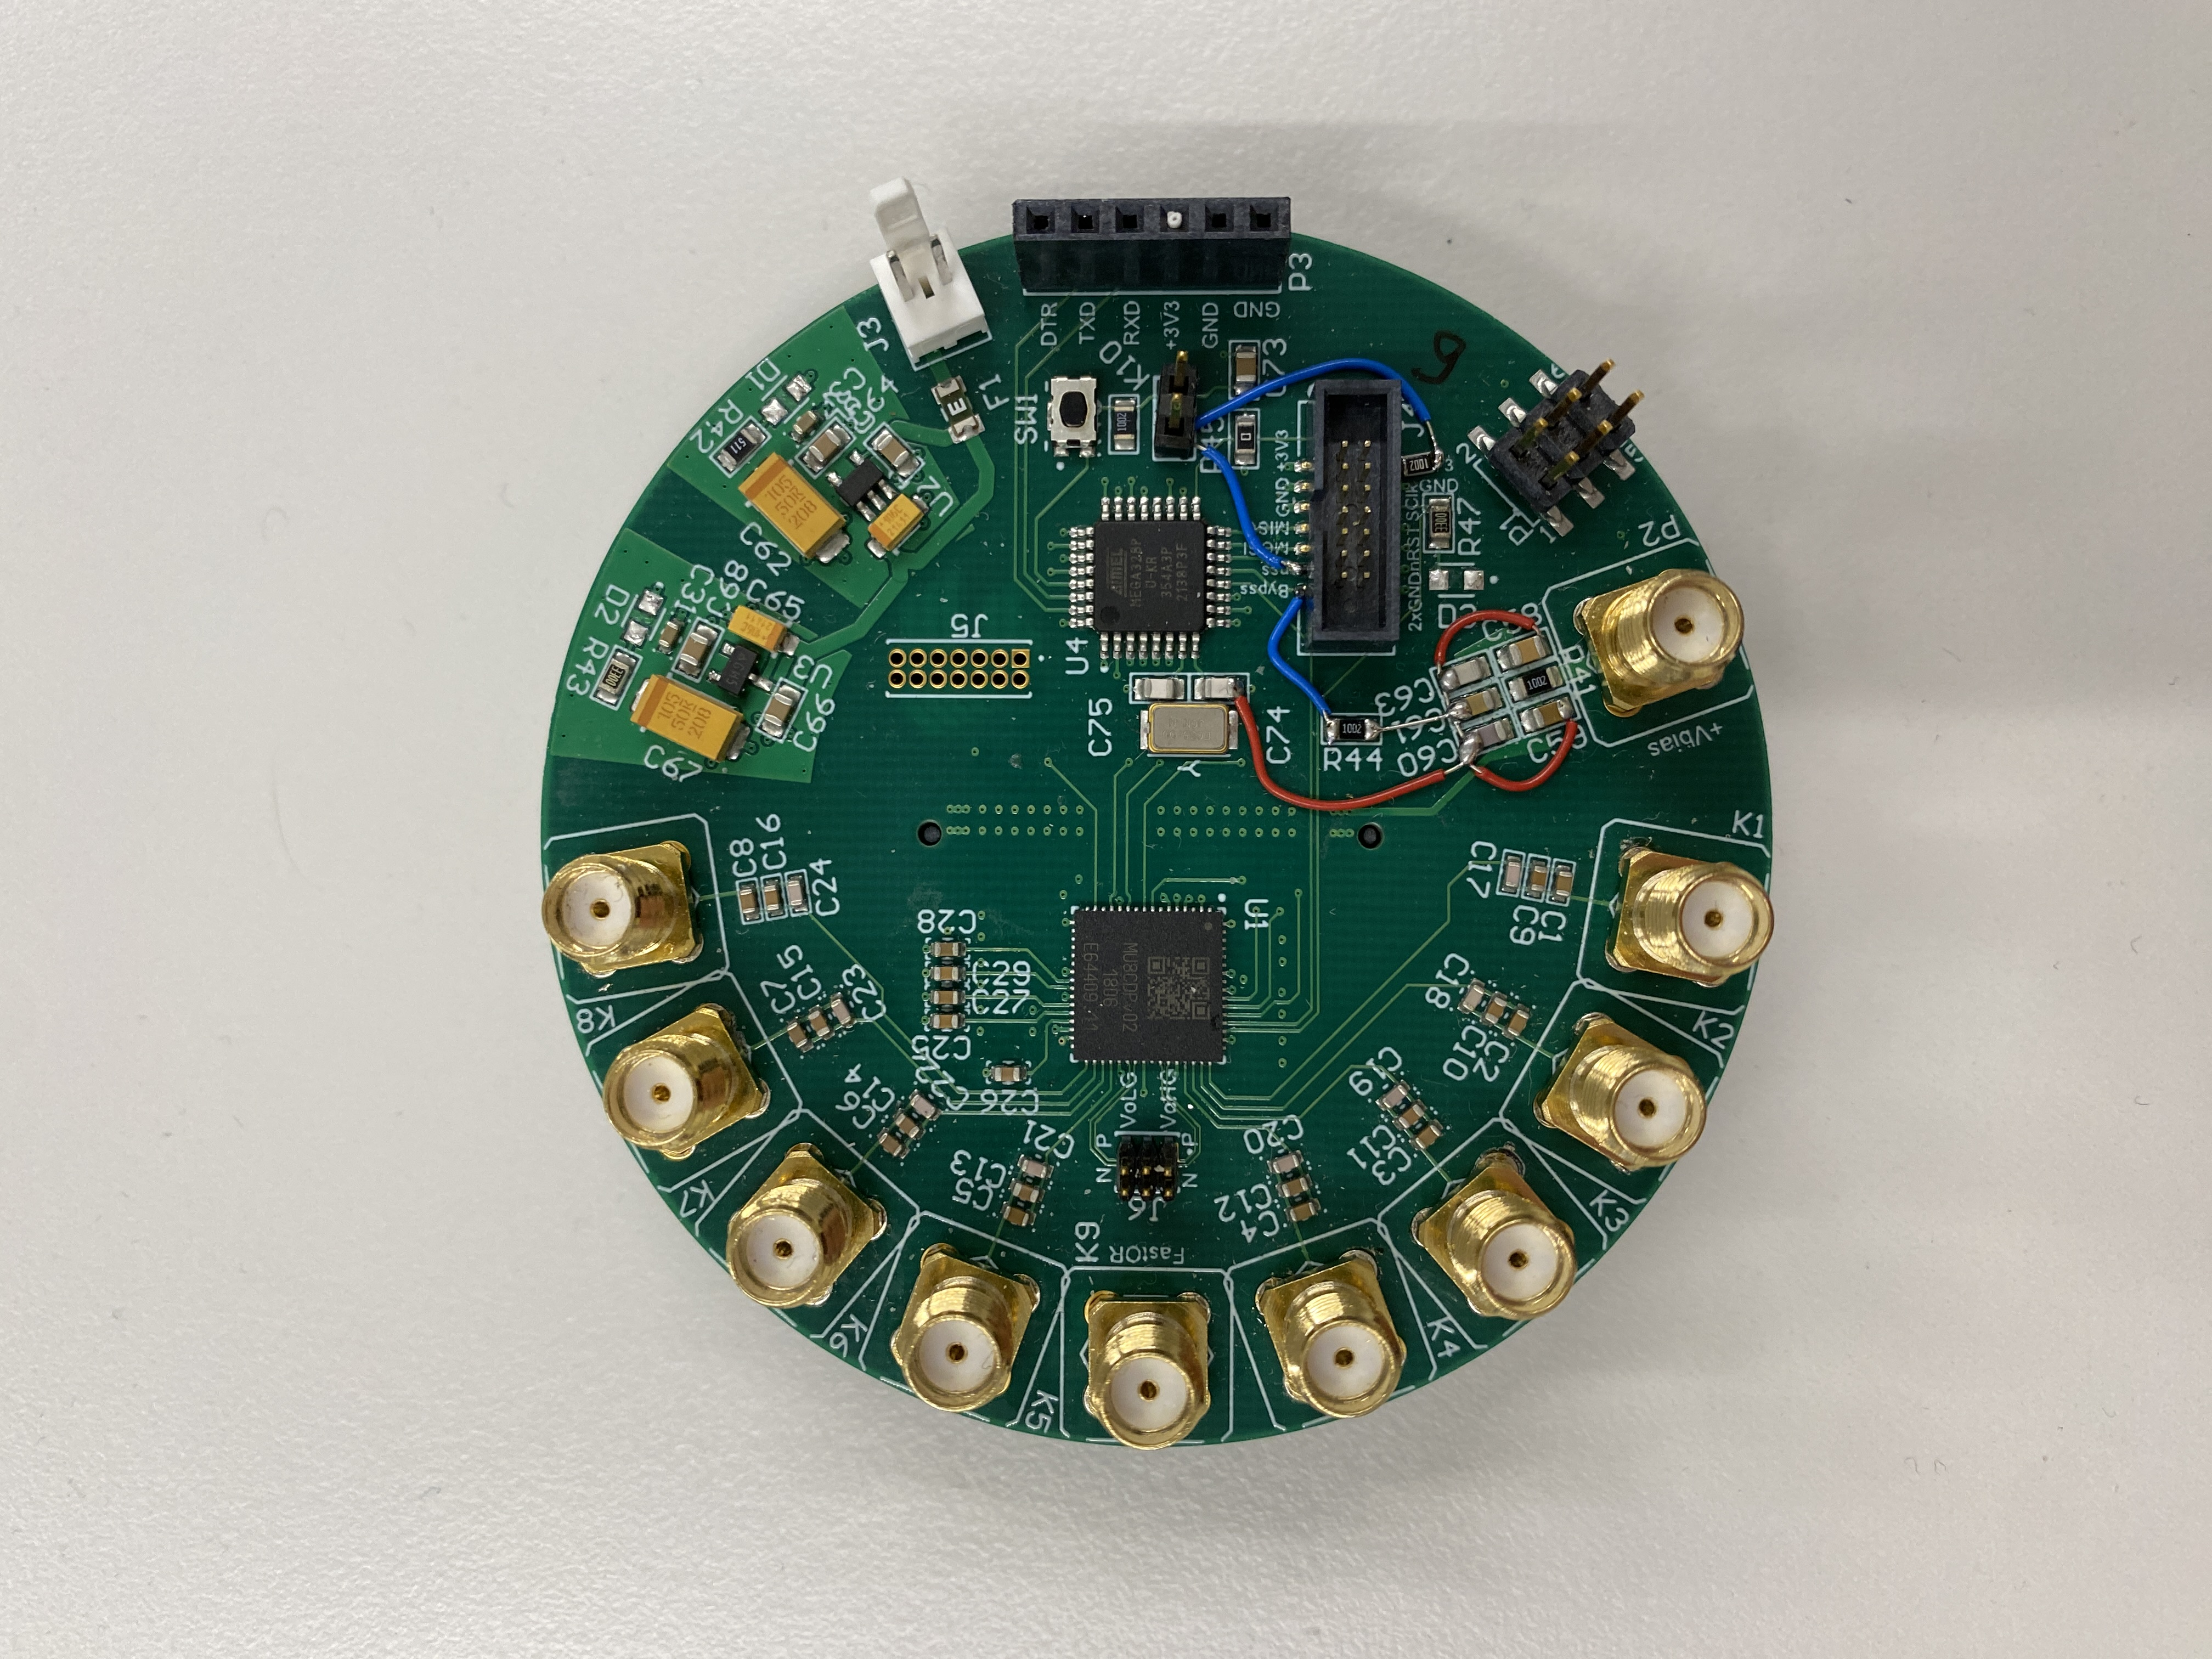
\includegraphics[width=1.\textwidth]{pictures/emusic_board}
	\caption[eMUSIC Board]{Picture of the \ac{emusic} board with the \ac{emusic} \ac{asic}, the eight single-ended channel-by-channel SMA signal outputs, the SMA fast OR output, the differential signal output, the SMA connector for the high voltage supply of the \acp{sipm}, and the connectors to program and power the board.}
	\label{fig:emusic_board}
\end{figure}





\section{The GANDALF Module}
The amplified and shaped output signal of the \ac{emusic} \ac{asic} needs to be digitized.
This step is done by GANDALF modules.
Originally developed at the University of Freiburg for the \ac{compass} experiment, it has a modular design to fill different roles in the experiments \ac{daq}.
Using mezzanine cards, different signal, clock, and trigger inputs can be chosen.
In the following, the GANDALF module will be introduced.
The mezzanine cards not used in this work are therefore only mentioned but not presented in detail.
An overview of a GANDALF module is shown in \autoref{fig:gandalf_overview}.
\begin{figure}
	\centering
	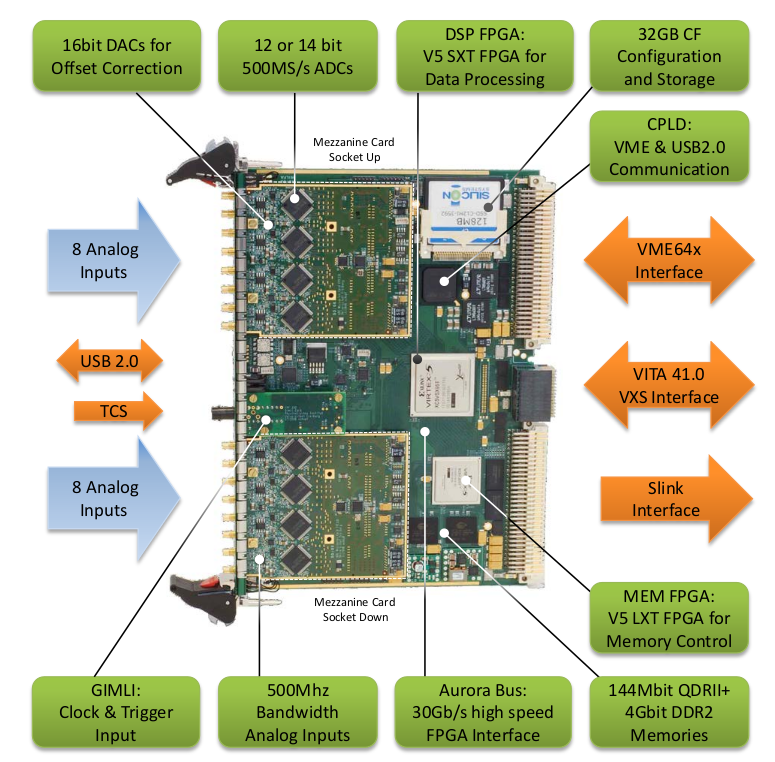
\includegraphics[width=.8\textwidth]{pictures/gandalf_overview.png}
	\caption[Overview of the GANDALF module]{Overview of the GANDALF module equipped with Analog Mezzanine Cards (AMCs) and the fiber Gimli mezzanine card for clock and trigger input. The analog waveforms are digitized by the AMCs, and the digitized data is processed by the DSP FPGA. The MEM FPGA handles the memory of the processed data, which can be transferred to a computer via the USB interface on the front of the VME or S-Link interfaces on the backplane. \cite{herrmann}}
	\label{fig:gandalf_overview}
\end{figure}

\subsection{Input Mezzanine Cards}
The GANDALF module has two mezzanine card slots for input signals.
For these slots, three different mezzanine cards were developed, \ac{amc}, \ac{dmc}, and \ac{omc}.
First, the last two mezzanine cards are shortly presented for completeness but are not relevant to the work done in this thesis.

\paragraph{The \ac{dmc}} has 64 digital inputs. 
%A picture of it is shown in \autoref{fig:dmc}.
Using either the LVDS or the LVPECL signal standard, one can use the DSP-\ac{fpga} logic for tasks like trigger decisions, time-to-digital conversion, or pattern generators, to name a few.
By changing the direction of the input buffer on the \ac{dmc} \ac{pcb}, the 64 channels of the \ac{dmc} can be used as outputs instead of inputs.

\paragraph{The \ac{omc}} has four \SI{3.25}{\giga\bit\per\second} transceivers to receive digital information, which can be further processed by the DSP-\ac{fpga}.
With this mezzanine card, the GANDALF can be used, for example, to merge data or as a concentrator.
%A picture of a \ac{omc} is shown in \autoref{fig:omc}.

\paragraph{The \ac{amc}} is designed to digitize analog input signals.
For digitization, eight \ac{adc} are used.
There are \ac{amc} with two different \ac{adc} available.
One is the \textit{ADS5463}, with \SI{12}{\bit} and up to \SI{500}{\mega\sample\per\second}, and the other is the \textit{ADS5474} which samples with up to \SI{400}{\mega\sample\per\second} at \SI{14}{\bit}.
The \ac{enob} of both \acp{adc} are \SI{10.4}{\bit} and \SI{11.2}{\bit}, respectively.
Each \ac{amc} has eight SMC connectors for the inputs.
There are \ac{amc} operating in \textit{normal mode}, meaning each SMC connector is connected to one \ac{adc}, resulting in eight channels with up to \SI{500}{\mega\sample\per\second} or \SI{400}{\mega\sample\per\second} per \ac{amc}.
In order to increase the sampling frequency, \acp{amc} which operate in the \textit{interleaved mode} were built.
On these \acp{amc}, four inputs are connected to two \ac{adc}s each, and therefore every second SMC connector is a dead end.
The clock signals which provide the sample tact for the two \acp{adc} of one channel have \SI{180}{\degree} phase offset with respect to each other.
By this, the sampling frequency is doubled to up to \SI{1}{\giga\sample\per\second} or \SI{800}{\mega\sample\per\second}, but the number of channels per \ac{amc} is reduced from eight to four.
The dynamic input range of the \ac{amc} is \SI{4.4}{\vpp} and can be shifted from the negative unipolar range \SIrange{-4.4}{0}{\volt} up to the bipolar range \SIrange{-2.2}{2.2}{\volt}.
This shifting is done by an \textit{AD5665R}, a \SI{16}{\bit} \ac{dac}.
The dynamic range was chosen because in the COMPASS experiment, for which the GANDALF was developed, negative voltage pulses created by \acp{pmt} needed to be digitized.
However, because the used \acp{adc} expect positive differential signals, inverting operational amplifiers are used to change the polarity of the signal.
By changing the gain of the amplifiers, one can decrease the input range and therefore increase the amplitude resolution.
The \acp{amc} used in this thesis are \SI{12}{\bit} \acp{amc} in the \textit{interleaved mode} and a dynamic range of \SI{2.2}{\vpp}.


\subsection{GIMLI Mezzanine Cards}
The third mezzanine card slot is for the GIMLI mezzanine cards, which are responsible for the clock and external trigger signals.
For this mezzanine card, three different options were developed.
One GIMLI card, which takes the clock and trigger from the backplane, if one wants to use the create to distribute the signals.
The fiber GIMLI has one fiber input to receive the clock and trigger via optical fiber.
And the copper GIMLI, which was used for this work and is presented in the following.

The copper GIMLI, shown in \autoref{fig:copper_gimli}, provides the option to use an external or an internal clock.
If only one GANDALF module is used, the internal \SI{20}{\mega\hertz} clock of the copper GIMLI can be used.
It is provided by an onboard oven-controlled oscillator (OCXO) with a jitter of less than \SI{2.3}{\pico\second}.
In case two or more GANDALFs are used, an external clock is required to ensure a synchronized clock on all GANDALF modules.
For this case, the copper GIMLI has a LEMO connector as input for an external clock with \ac{nim} signal standard.
Via a second LEMO connector, an external \ac{nim} trigger signal can be connected to the GANDALF module.

\begin{figure}
	\centering
	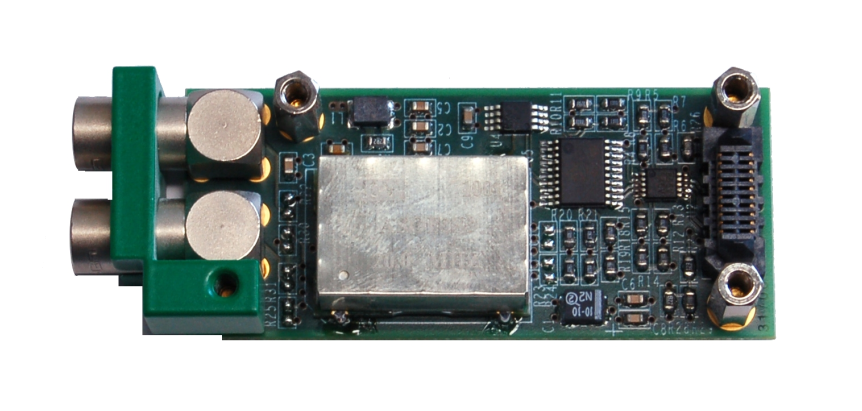
\includegraphics[width=.5\textwidth]{pictures/copper_gimli.png}
	\caption[Copper GIMLI]{Picture of the copper GIMLI with an internal \SI{20}{\mega\hertz} clock generated by an onboard oven-controlled oscillator. With the LEMO connectors external clock and trigger \ac{nim} signals can be provided for the GANDALF. \cite{herrmann}}
	\label{fig:copper_gimli}
\end{figure}



\subsection{Usage of the GANDALF with \acp{sipm}}
In this work, the GANDALF was used for digitizing the output signal of the \ac{emusic} \ac{asic}.
As mentioned above in \autoref{sec:emusic}, these signals have a positive polarity.
But because the GANDALF was designed for the digitization and processing of negative voltage pulses created by a \ac{pmt}, this caused some problems.
Since after the inverting operational amplifiers in the GANDALF, the \ac{sipm} signals have a negative polarity, the input voltage range needs to be chosen to be bipolar and around \SIrange{-1.1}{1.1}{\volt}.
%In order to get this input range the baseline at \SI{0}{\volt} would need to be set to \SI{2047}{\adcu}.
%For unknown reasons the programm which configeres the \acp{dac} to set the baseline to a \si{\adcu} value selectable by the user will set the baseline to a maximum of around \SI{1400}{\adcu}.
%With $\frac{2.2}{2^12}\,\si{\volt\per\adcu} = \SI{0.537}{\milli\volt\per\adcu}$ the range of the inverted signal is \SI{1400}{\adcu} which corresponds to approximately \SI{752}{\milli\volt}.
%Should this range be not enough, one needs to either try to find the source of the problem and fix it or decrease the amplification of the \ac{emusic} \ac{asic}.
%The next problem regards the self-trigger of the GANDALF.
Also, the self-trigger of the GANDALF needed to be adjusted.
It functions via samples over threshold.
The user can set a threshold and a number of consecutive samples which need to be over the threshold for the GANDALF to trigger an event.
Since after the inverting of the positive signals, the signals have a negative polarity, and the threshold needs to be set to a lower ADC value than the baseline.
In addition to that, the sample over threshold condition in the GANDALF firmware needed to be inverted to trigger if a number of consecutive samples were below the threshold.
The new firmware with the inverted trigger condition was tested and worked as intended, with the exception of one bug.
If the data rate from the GANDALF to the \ac{daq} computer exceeds the maximum possible data rate, \SI{20}{\mega\byte\per\second} in the case of the USB interface, incomplete events will be written down to disk.
This is most likely caused by a missing VHDL file that was not included in the new firmware and which would, in case the buffer of the GANDALF is completely filled, prevent the GANDALF from sending incomplete events to the computer.
For the intended use of this bug should not be a problem since the data rate is expected to be way below the possible \SI{20}{\mega\byte\per\second}.

%\chapter{Setup}

% dark box
% power supplies
% multimeter
% osci
% gandalf + clock
% led + diffusor
% emusic
% sipm
\section{SiPM}
An important part of the setup are of course the \acp{sipm} which generate the charge signal which than gets amplified by the \ac{emusic} chips.
The \acp{sipm} mainly used in this work are the \textit{S14160-3050HS} by the manufacturer Hamamatsu.
Another \ac{sipm} model which was used at the \ac{desy} testbeam besides the \textit{S14160-3050HS} is the SensL \textit{J-Series 30035} manufactured by Onsemi.
Some important parameters of both \ac{sipm} models are listed in \autoref{tab:sipm_specs}.
For this work, \acp{pcb} with forty \acp{sipm} soldered onto it were used.
These boards exist with both \ac{sipm} models.
A picture of one of these \acp{pcb} equiped with Hamamatsu \acp{sipm} is shown in \autoref{fig:sipm_pcb}.
A breakout board can be plugged in on the back of the \ac{pcb}.
For this thesis the \ac{emusic} board was used as a breakout board, which is described in the previous chapter.
\begin{table}
	\centering
	\caption[SiPM parameters]{Relevant parameters of the both used \ac{sipm} models by Hamamatsu and Onsemi. \cite{}}
	\label{tab:sipm_specs}
	\renewcommand{\arraystretch}{1.3}
	\begin{tabularx}{\textwidth}{Xp{0.19\textwidth}p{0.15\textwidth}}
	    \toprule
	    parameter								& S14160-3050HS		& SensL			\\\midrule
	    photosensitive are / $\si{\milli\meter\squared}$			& 3.0$\times$3.0	& 3.07$\times$3.07	\\
	    pixel pitch / $\si{\micro\meter}$					& 50			& 35			\\
	    number of pixels							& 3000			& \num{5676}		\\
	    spectral response range / $\si{\nano\meter}$			& \numrange{270}{900}	& \numrange{200}{900}	\\
	    peak sensitivity wavenlength / $\si{\nano\meter}$			& 450			& 420			\\
	    peak photon detection eficiency / $\si{\percent}$			& 50			& 			\\
	    breakdown voltage / $\si{\volt}$					& 38			& \numrange{24.2}{24.7}	\\
	    recommended operating voltage / $\si{\volt}$			& 40.7			& \numrange{25.2}{30.7}	\\
	    variation of rec. op. voltage (typ. / max) / $\si{\volt}$		& 0.1 / 0.2		&			\\
	    gain								& \num{2.5e6}		&			\\
	    \bottomrule
	\end{tabularx}
	\renewcommand{\arraystretch}{1}
\end{table} 
\begin{figure}
	\centering
	\includegraphics[width=.5\textwidth]{pictures/sipm_ham_pcb}
	\caption[\ac{pcb} with Hamamatsu \acp{sipm}]{One of the \acp{pcb} with Hamamatsu \acp{sipm} used for this work.}
	\label{fig:sipm_pcb}
\end{figure}

\section{Dark Box Setup}
To ensure a controlled evironment for the measurements, the \acp{sipm} were placed inside a dark box.
The inside of the box is covered in black aluminum foil made by Thorlabs with a reflectivity in the visible wavelength spectrum below \SI{5}{\percent} \cite{}.
An optical rail for fixing the \ac{sipm} board, a diffusor and the end of an optical fiber was placed in the box.
Via the optical fiber the light of a \SI{460}{\nano\meter} LED can be guided into the box.
The LED is inside of another light tight box.
It was build as part of the bachelor thesis of Alexander Bismark and is described there in more detail \cite{}.
Power can be supplied to the LED via a BNC connector on the light tight box.
In this thesis the Tektronix AFG was used to create voltage pulses with a width down to \SI{4}{\nano\second} with \SI{2.5}{\nano\second} rising and falling edges.
To eluminate all \acp{sipm} equaly a \textit{ED1-C50-MD} diffuser by Thorlabs was used.
A light beam hitting the diffusor perpendicular to its surface gets diffused in a circular shape with a \SI{50}{\degree} opening angle.
%The relative light intensity of the diffused light of a collimated \SI{488}{\nano\meter} laser beam measured by Thorlabs is shown in \autoref{fig:diffuser_dist} \cite{}.

Multiple BNC, SMA, and SMC feedthroughs were installed in the dark box to supply the \acp{sipm} and \ac{emusic} board with power and to transfer the output signals of the \ac{emusic} out of the box to a digitizer or oscilloscope.
Also a hole drilled to insert the optical fiber from the LED setup into the box and afterwards covered, to block light from entering through the hole.
A power supply was used for the high voltage supply of the \acp{sipm}.
If not otherwise specified, all measurements shown in this thesis were done with a high voltage of \SI{43}{\volt}.
To control the voltage the HP multimeter was used instead of the less precise voltage display of the power supply.
The \ac{emusic} board was powered by a \SI{8}{\volt} power supply.
For the digitization either a \ac{gandalf} or the Tektronix oscilloscope was used.

\autoref{fig:setup_sketch} shows a schmatic sketch of the setup inside and on the outside of the box.
A picture of the setup inside the box is shown in \autoref{fig:setup_box_pic}.
It includes the LED fiber, the diffuser, the \ac{sipm} and \ac{emusic} board with power and signal cables attached.
In the following the setup part with the \ac{gandalf} is described.
\begin{figure}
	\centering
	\includegraphics[]{}
	\caption[]{}
	\label{fig:setup_sketch}
\end{figure}
\begin{figure}
	\centering
	\includegraphics[width=0.5\textwidth]{pictures/setup_box_pic}
	\caption[Picture of the inside of the dark box.]{The inside of the dark box which was used for the test measurements. On the left is the end of the fiber from the LED setup mounted on the optical rail. Behind the fiber end is a diffuser by Thorlabs which diffuses the light in a circular distribution with an opening angle of \SI{50}{\degree}. After the diffuser is the \ac{pcb} with the \acp{sipm} placed. On its back is the \ac{emusic} board plugged in. The high voltage for the \acp{sipm} is supplied via the brownish cable, the power for the \ac{emusic} chip is supplied with the red and black cable and the signal outputs of the \ac{emusic} boards are connected with the feedthrough on the box via the black SMA cables.}
	\label{fig:setup_box_pic}
\end{figure}

\section{Gandalf}

For the operation of the One Cell Prototype sixteen channels need to be digitized, eight of each of the two \acp{wom}.
Therefore two \acp{gandalf} are required.
In order to save place and simplify the setup, the \acp{gandalf} are not operated in a VME crate but are each in a \ac{gandalf} portable.
It is a mobile case made exactly for such puroses where a whole crate is unconvinient.
A picture of a \ac{gandalf} portable is shown in \autoref{fig:gandalf_portable}.
Due to the usage of two \acp{gandalf} an external clock is required to ensure a syncronized sampling frequency and clock for time stamps.
As an external clock a copper GIMLI was chosen and used with a GIMLI testboard, shown in \autoref{fig:gimli_testboard}.
It has two slots for GMILIs, for each on data and one clock output and a power connector to supply it with \SI{5}{\volt}.
For the purpose of an external clock, only one of these slots and the corresponding clock output is used.
Via LEMO cables, the clock signal form the boards clock output pins is connected to the clock inputs of the \acp{gandalf}.
\begin{figure}
	\centering
	\begin{subfigure}[b]{.4\textwidth}
		\centering
		\includegraphics[width=1.\textwidth, angle=-90]{pictures/gandalf_portable} 
		\caption[A \ac{gandalf} portable equiped with a \ac{gandalf}.]{}
		\label{}
	\end{subfigure}
	\begin{subfigure}[b]{.55\textwidth}
		\centering
		\includegraphics[width=1.\textwidth]{pictures/gimli_testboard}
		\caption[]{}
		\label{}
	\end{subfigure}
	\caption[]{A \ac{gandalf} portable equiped with a \ac{gandalf}. The GIMLI test board with a copper GIMLI}
	\label{}
\end{figure}

%\chapter{Results of the \ac{daq} tests}


\section{GANDALF Clock Frequency and ADC Test}
Before using the \ac{gandalf} modules in the \ac{daq}, they need to be tested.
For this to things are relevant.
One of these is the sample frequency, if it correspondes to the theoretical sample frequency.
The other is the test of the \acp{adc} to see if they have dead bits or other malfunctions.
To perform this test a \SI{150}{\mega\hertz} sin voltage signal was generated with an AWG and a \SI{150}{\mega\hertz} filter by XXXXXXX was used.
This filter ensures that the sin signal is clean and no unwanted frequencies are present.
The clean sin signal was than connected to the inputs of the \acp{gandalf}, one after another.
For each input \num{1000}1000 measurements were done each with XXXXX samples.
For each channel a \ac{fft} was done for one waveform using the python3 functions \textit{scipy.fft.rfft} and \textit{scipy.fft.rfftfreq} to find the frequencies in the signal.
\autoref{fig:gandalf_input_g23_ch0} shows the plot with the \ac{fft} for channel 0 of the \ac{amc} 46 used with the \ac{gandalf} 24.
In the plot the red line marks the \SI{150}{\mega\hertz} of the sin signal and the green line marks the peak frequency of the measured signal.
The measured values and the corresponding uncertainties are listed in \autoref{tab:gandalf_sin_150}.




To test if the bits in the \acp{adc} are working, the amplitudes of all samples of every waveforms in a measurement were put into histogram.





\section{Input Offset Voltage}
The first measurement with the \ac{emusic} board is to find out the input offset voltage of the \ac{emusic} for different \ac{dac} values.
This needs to be done to find out the exact overvoltage of the \acp{sipm}, which influences among other things the gain of the \acp{sipm}.
In order to perform this measurement, the setup in \autoref{fig:input_offset_setup} was assembled.
The \ac{emusic} board was powered by the \SI{8}{\volt} power supply and the XXXXXXXX power supply was used to supply the high voltage.
It was set to \SI{4.7}{\volt} since it was not important for the high voltage to be over the breakdown voltage of the \acp{sipm}.
It should only be over the maximum input offset the \ac{emusic} can generate for the resulting voltage to be applied in reverse direction to the \acp{sipm}.
For this measurement the \ac{emusic}s input \ac{dac} settings, which can range from 0 to 511, were set to 0.
Then the voltages between the negative high voltage pole and the voltage on the cathode of the \acp{sipm} were measured.
As measurement point for the cathode voltage, the \SI{0}{\ohm} resistor placed on the back of the \ac{sipm} board was chosen.
It is shown in \autoref{fig:meas_input_resistor}.
This measurement was done for one \ac{sipm} of each \ac{sipm} group.
The chosen \ac{sipm} were 1, 6, 11, 16, 21, 26, 31 and 36.
After measureing the voltages, the \ac{dac} setting was increased in steps of \SI{50}{\dacu} until \SI{500}{\dacu} and at each step the measurement was repeated.
In the following first the measurement results of the individual channels over all tested \ac{dac} settings are presented.
Afterwards, the input offset voltages of the different channels for the same setting are compared.

As an example, the measurements of all eleven tested \ac{dac} settings done with the \ac{emusic} board 2 and channel 0 are shown in \autoref{fig:input_offset_b2_ch0}.
In the upper part of the plot, the measured voltages are plotted and for the measurements with a \ac{dac} setting between \SI{100}{\dacu} and \SI{100}{\dacu} a linear fit was performed.
The first two measured voltages were not included, since they visibly do not follow the linear trend.
For all channels the first to measured values are at around \SI{1530}{\milli\volt} which indicates that in that \si{\dacu} range the different settings do not change the offset voltage.
Depending on the \ac{emusic} board and the channel also the last one or two measured voltages were excluded from the fit since they also do not follow the linear trend and increase to around \SI{940}{\milli\volt} instead of decreasing further.
The resulting slope and offset of the linear fit are
\begin{align}
    V_\text{offset, fit} &= \SI{-3.43(5)}{\milli\volt\per\dacu}\cdot x+\SI{1828(11)}{\milli\volt}
\end{align}
where x is the setting of the \ac{dac} in \si{\dacu}.
The bottom of the plot shows the residual plot where the difference between the linear fit and the measured values is shown.
The range on the y-axis is fixed to \SIrange{-20}{20}{\milli\volt}.
From that one can see, that should be a precission of \SI{+-20}{\milli\volt} sufficient for ones used, one can use the results from the linear fit to adjust the overvoltage.
In case one wants a precission in the single \si{\milli\volt} range, this is not suitable anymore.
Than the \ac{dac} needs to be adjusted while measureing the voltage on the inputs of the \ac{emusic} \ac{asic}.
In \autoref{tab:input_offset_linear_fit} the fit results for the measurements with the \ac{emusic} boards 2 and 6 are listed.
The \ac{dac} voltages of the channels differ to other channels on the same board as well as to the channels on the other board.
Therefore the measurement of the input voltage should be done for every \ac{emusic} board.
\begin{figure}
	\centering
	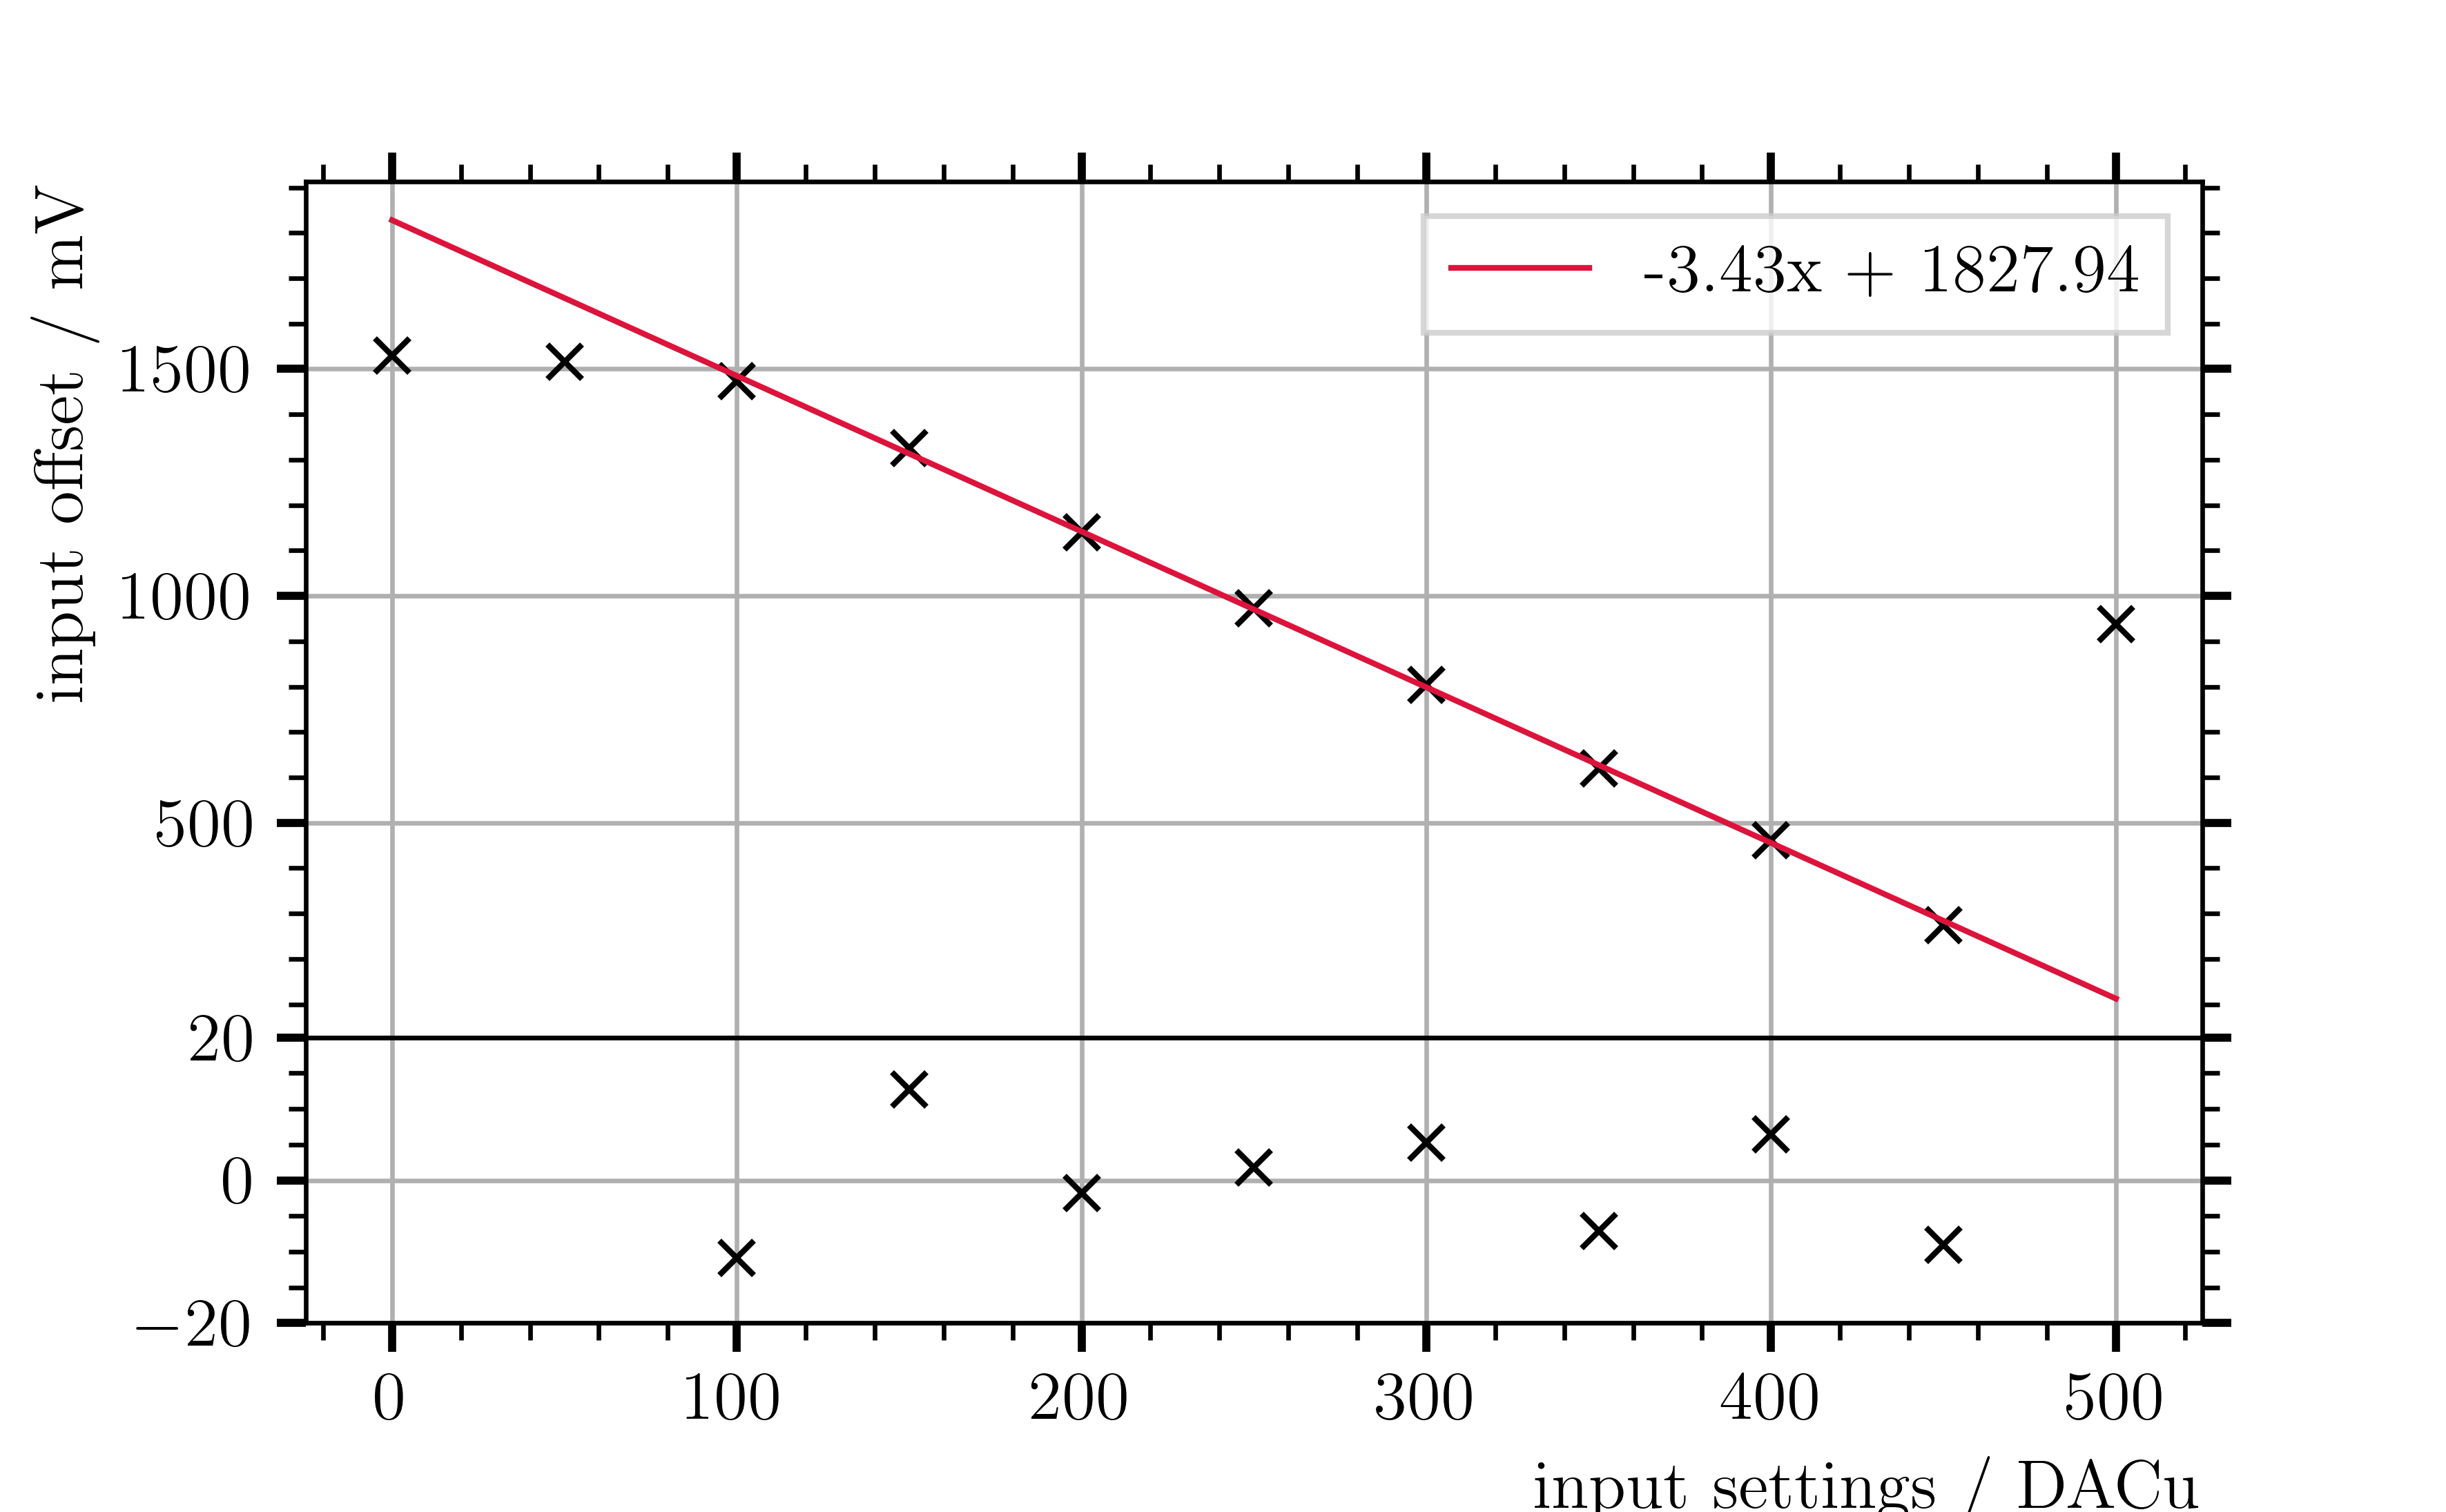
\includegraphics[width=1.\textwidth]{pictures/input_offset_board_2_channel_0}
	\caption[Input offset measurement for eMUSIC board 2 channel 1]{Input offset measurement for the channel 0 of the \ac{emusic} board 2. The input voltage was measured for input \ac{dac} settings from \SIrange{0}{500}{\dacu} in \SI{50}{\dacu} steps. A linear fit was performed for the measurements with \ac{dac} settings between \SI{100}{\dacu} and \SI{450}{\dacu}. The other measured voltages were excluded form the fit since they do not follow the linear trend. Below is the residual plot with a fixed y-axis window from \SI{-20}{\milli\volt} to \SI{-20}{\milli\volt}.}
	\label{fig:input_offset_b2_ch0}
\end{figure}
\begin{table}
	\centering
	\caption[todo]{todo}
	\label{tab:input_offset_linear_fit}
	\begin{tabular}{|c|c|c|c|}
		a & a & A & a
	\end{tabular}
\end{table}

To compare the differences between channels with the same \ac{dac} settings, for three different settings the input voltage was plotted for all eight channels in \autoref{fig:input_offset_b2_dac}, \autoref{fig:input_offset_b2_dac}, and \autoref{fig:input_offset_b2_dac}.
For settings at \SI{50}{\dacu} and below, the input offset voltage is pretty equal between the channels and only differs in the single \si{\milli\volt} range around \SI{0}{\milli\volt}.
A similiar behavior is seen for \ac{dac} settings at and above \SI{500}{\dacu}, for which the input voltage is around \SI{940}{\milli\volt} and the differences between the channels is also in the single \si{milli\volt} range.
But in the \si{dacu} range where the linear progression can be seen, the variations between the channels is larged, in some cases over \SI{70}{\milli\volt}.
This confirms, that the measurement of the input voltage needs to be done for all \ac{emusic} boards and all channels.
\begin{figure}
	\centering
	\begin{subfigure}[b]{1.\textwidth}
		\centering
		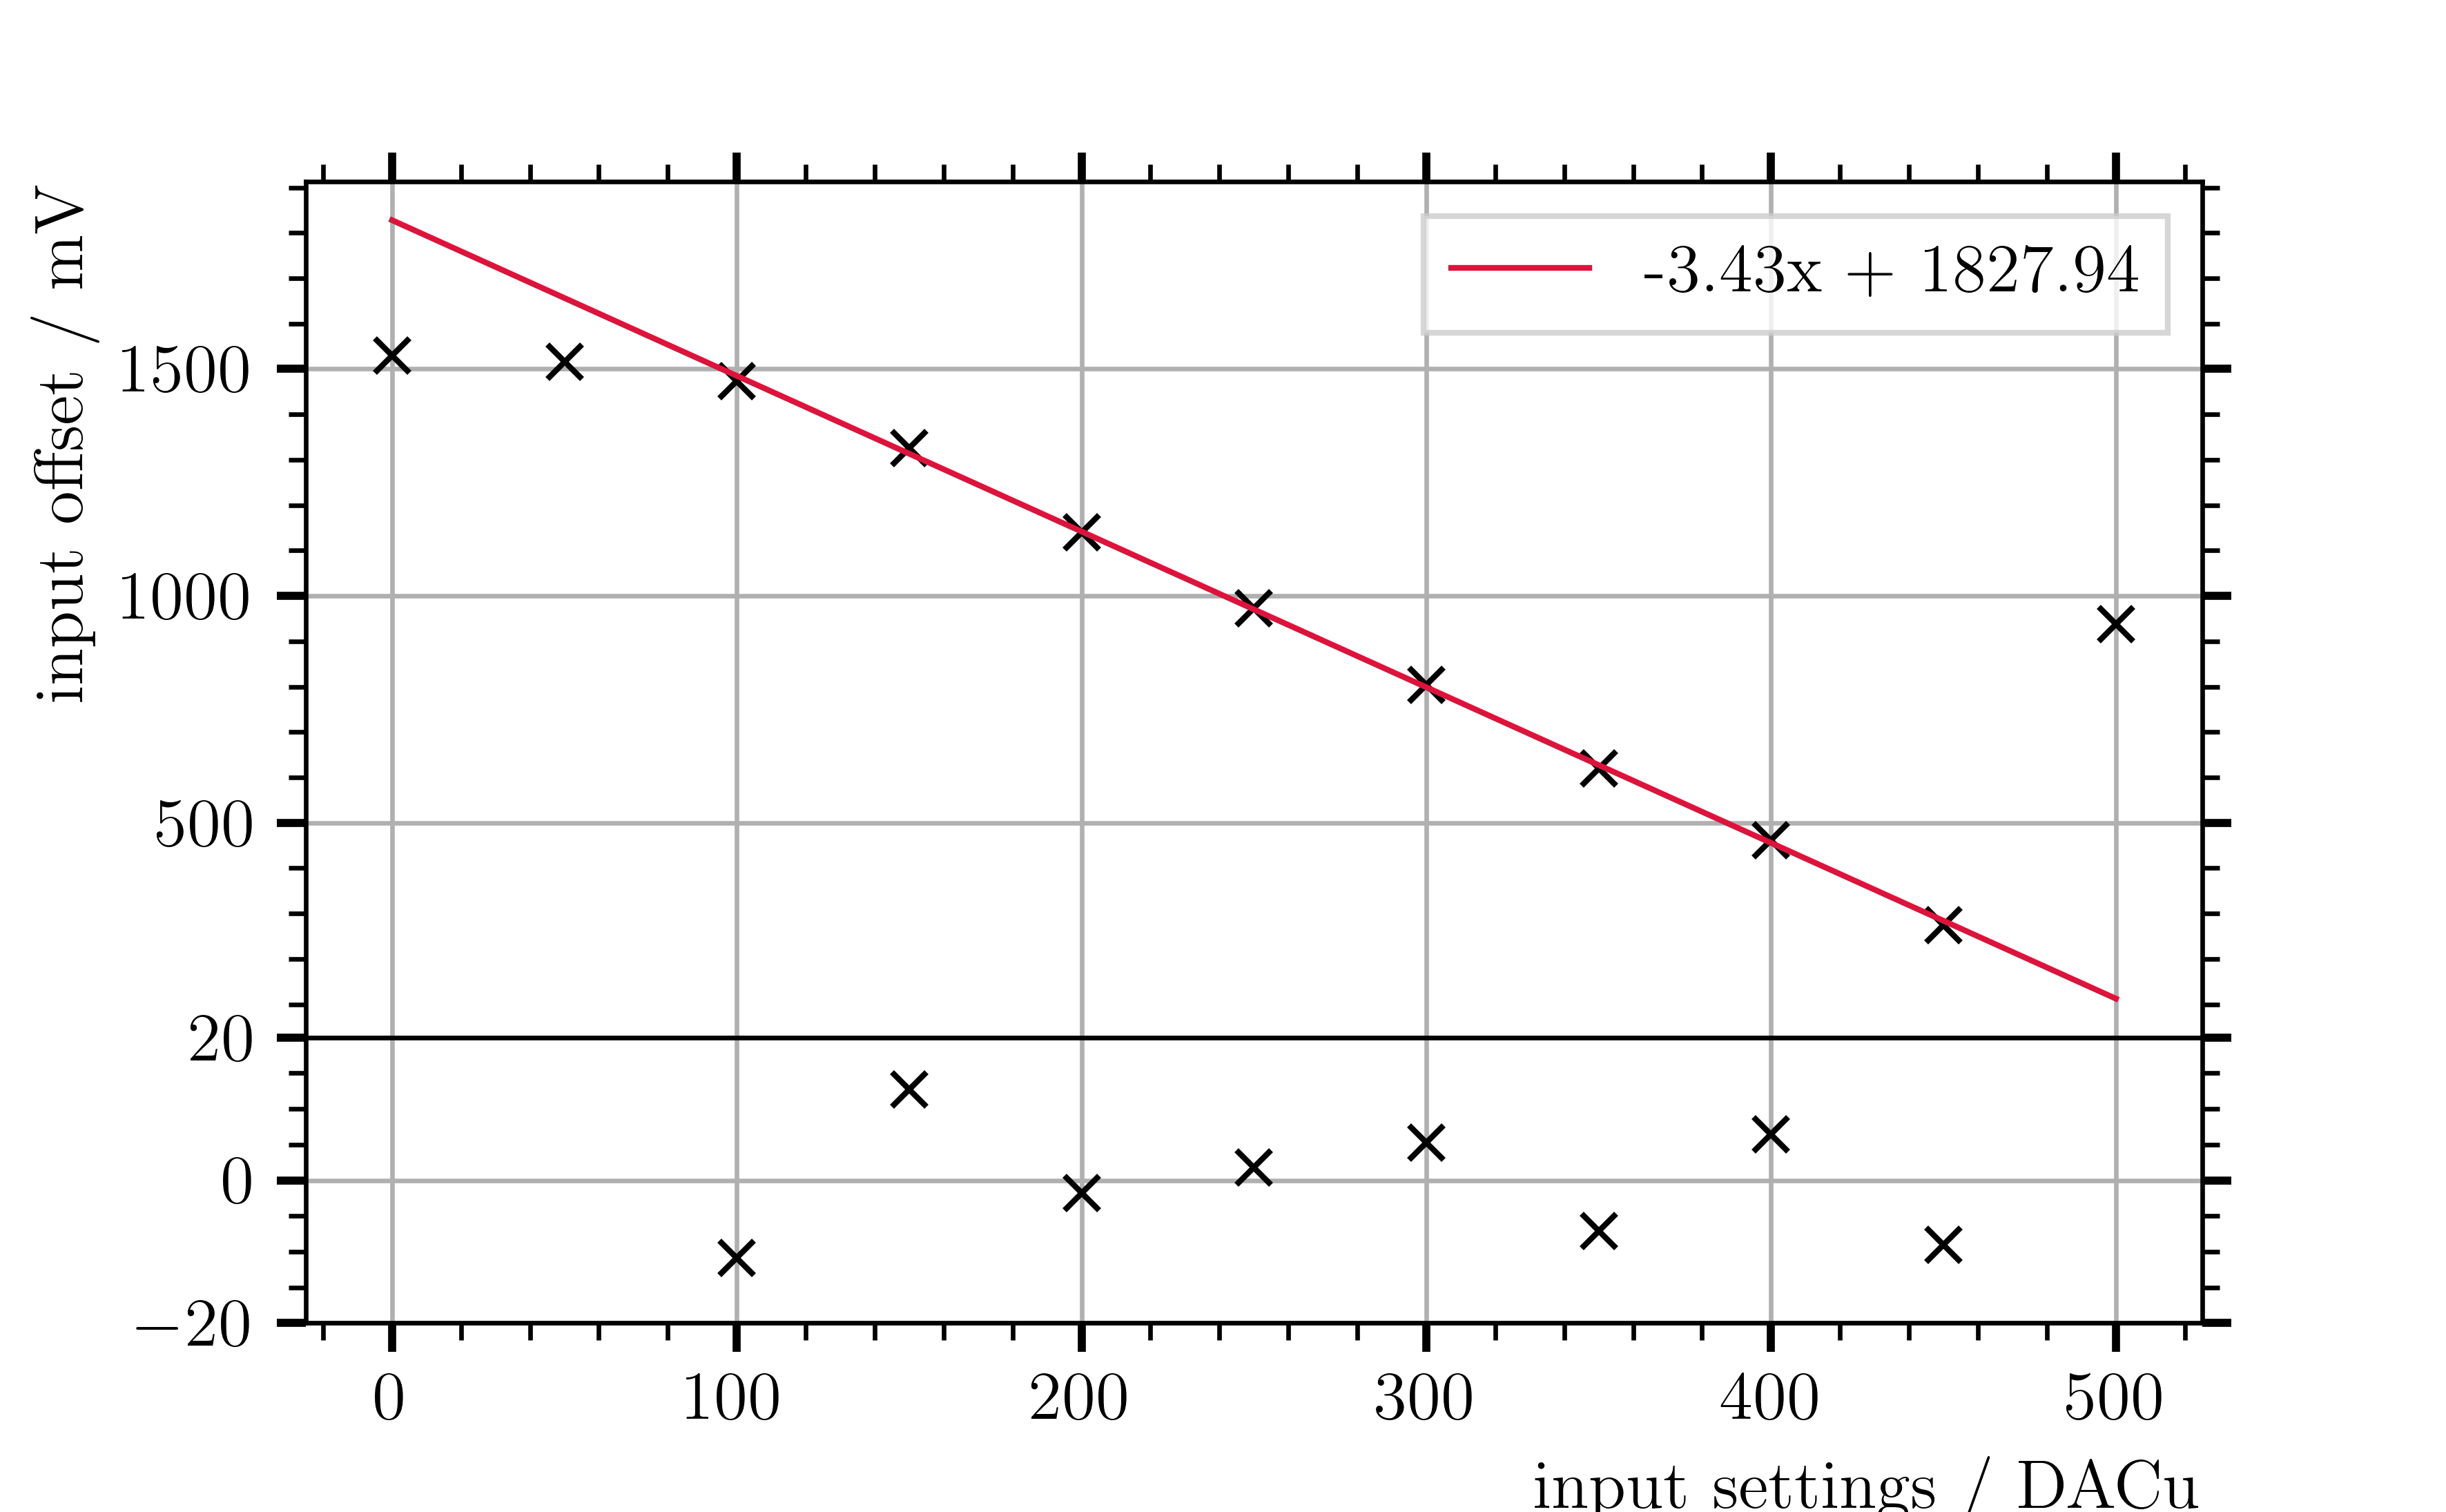
\includegraphics[width=.5\textwidth]{pictures/input_offset_board_2_channel_0.png}
		\caption{}
		\label{fig:input_offset_b2_dac50}
	\end{subfigure}
	
	\begin{subfigure}[b]{1.\textwidth}
		\centering
		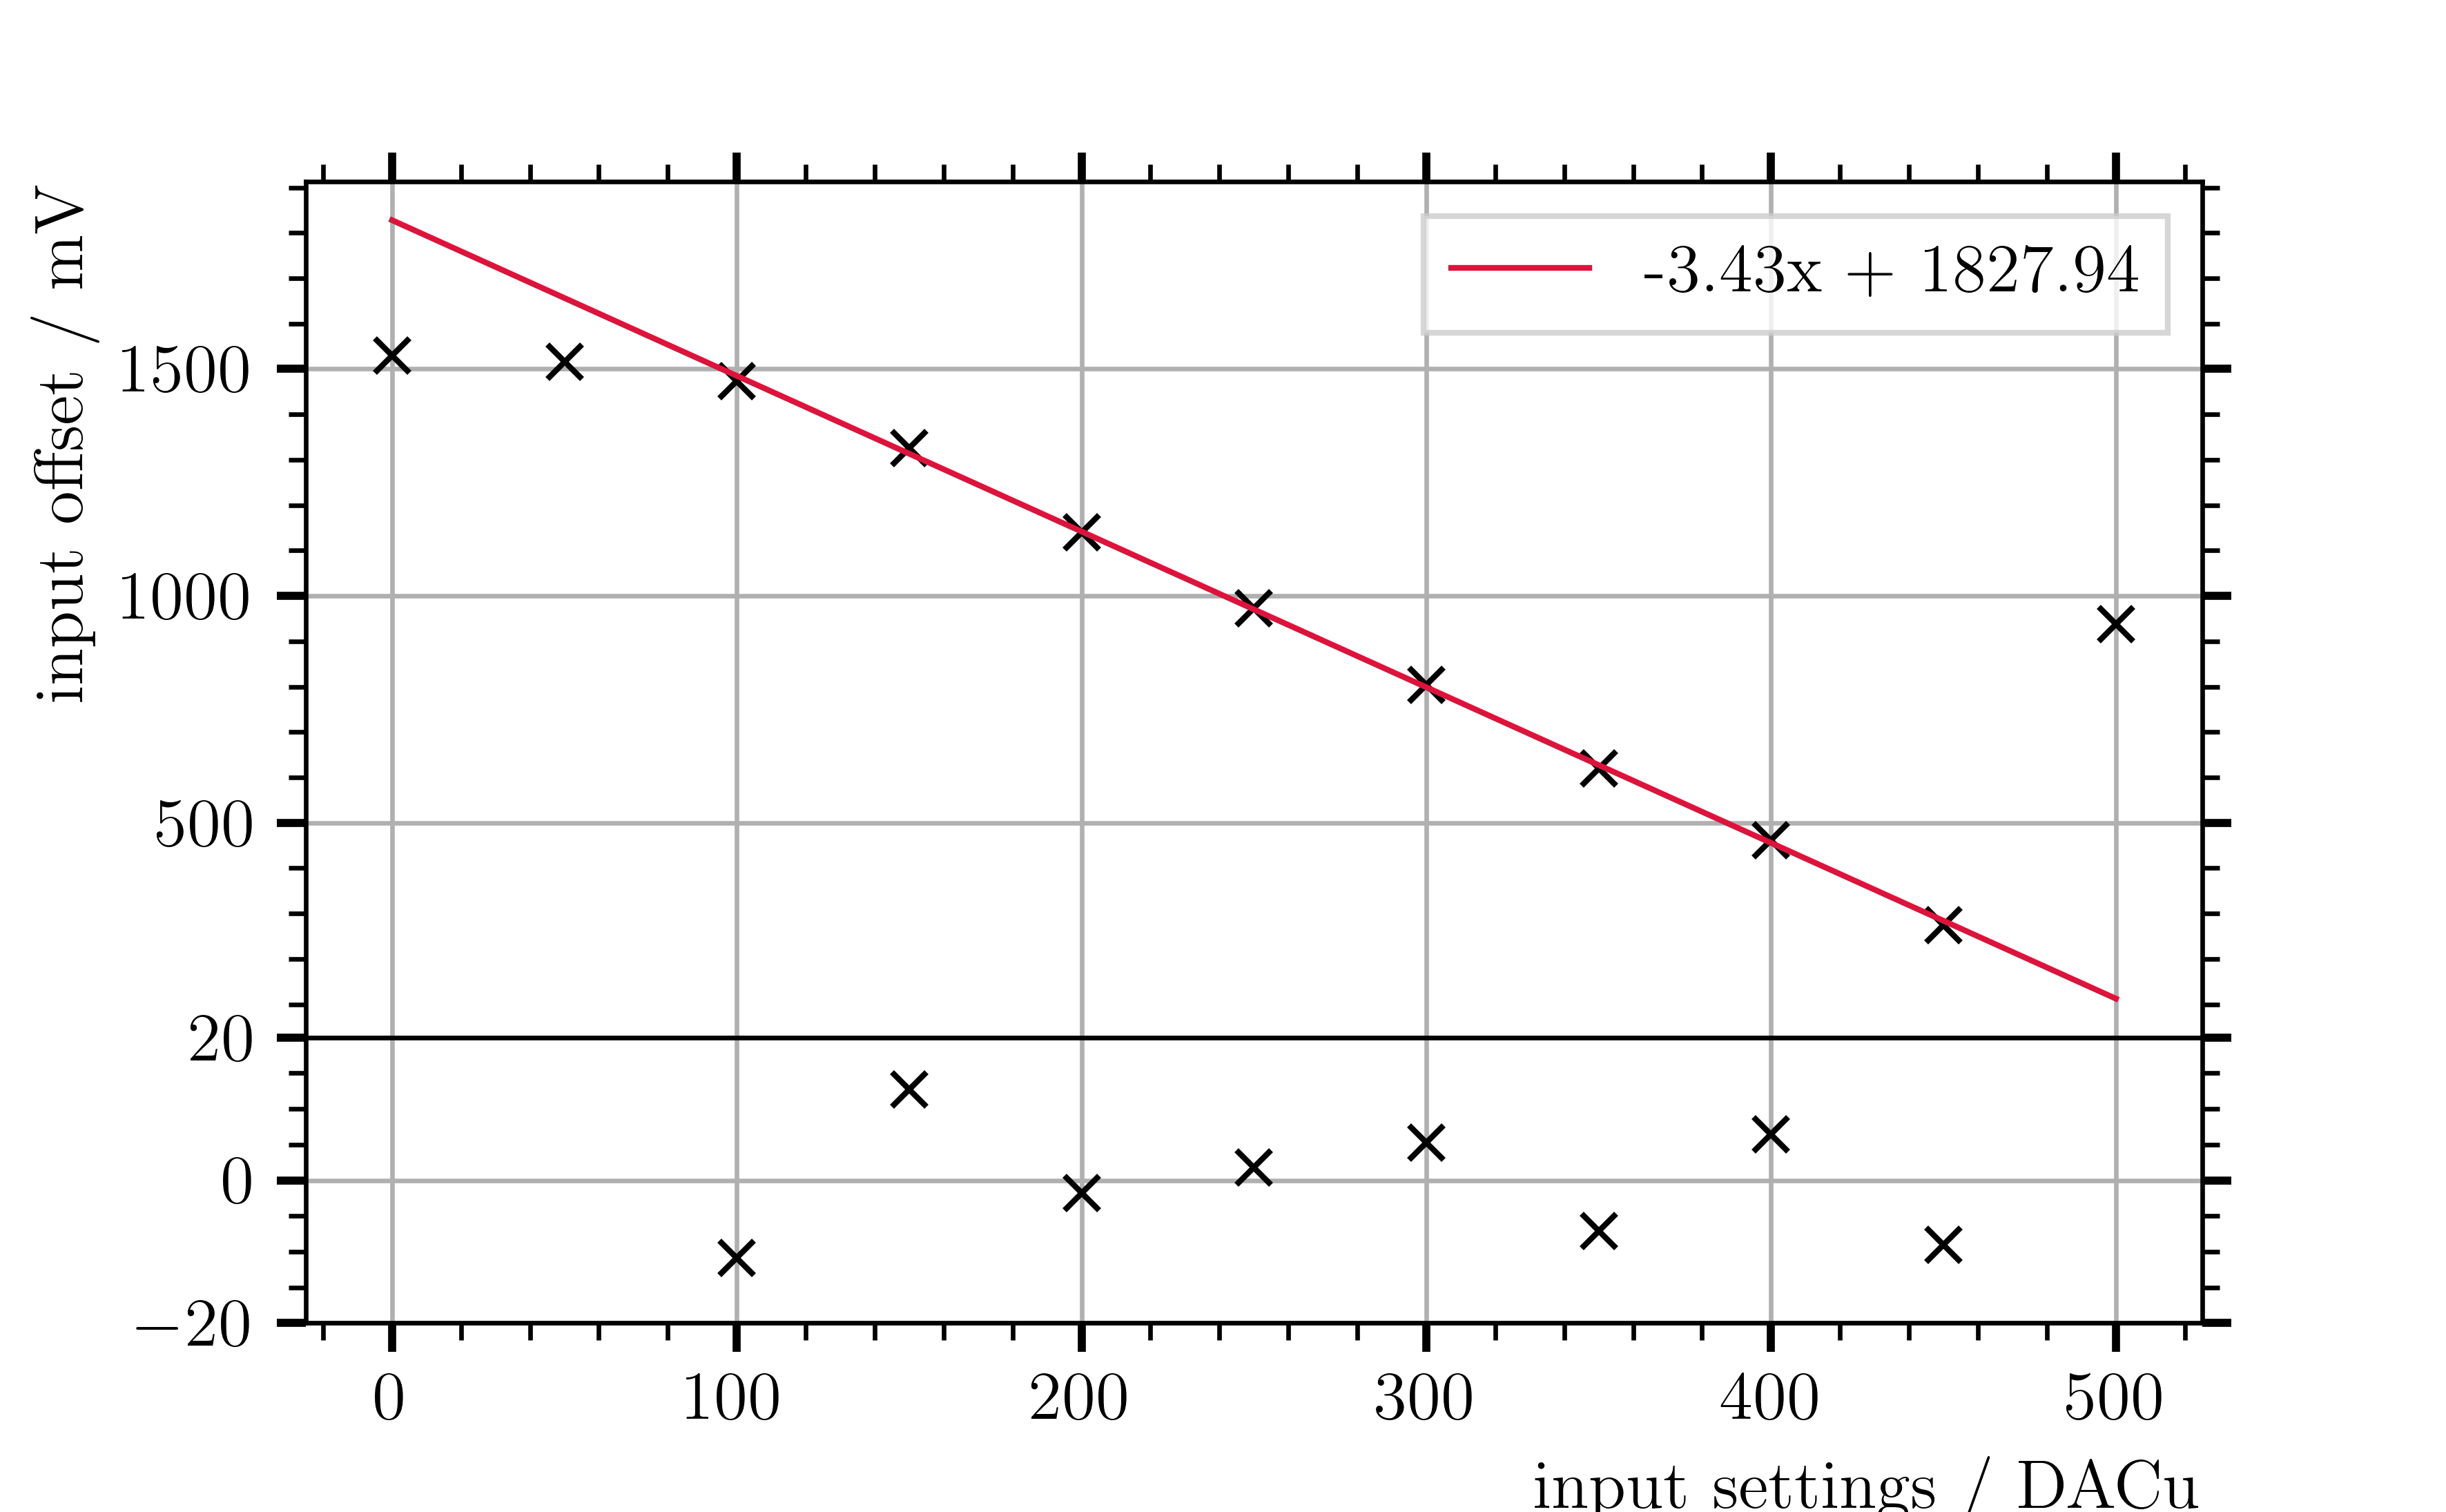
\includegraphics[width=.5\textwidth]{pictures/input_offset_board_2_channel_0.png}
		\caption{}
		\label{fig:input_offset_b2_dac50}
	\end{subfigure}

	\begin{subfigure}[b]{1.\textwidth}
		\centering
		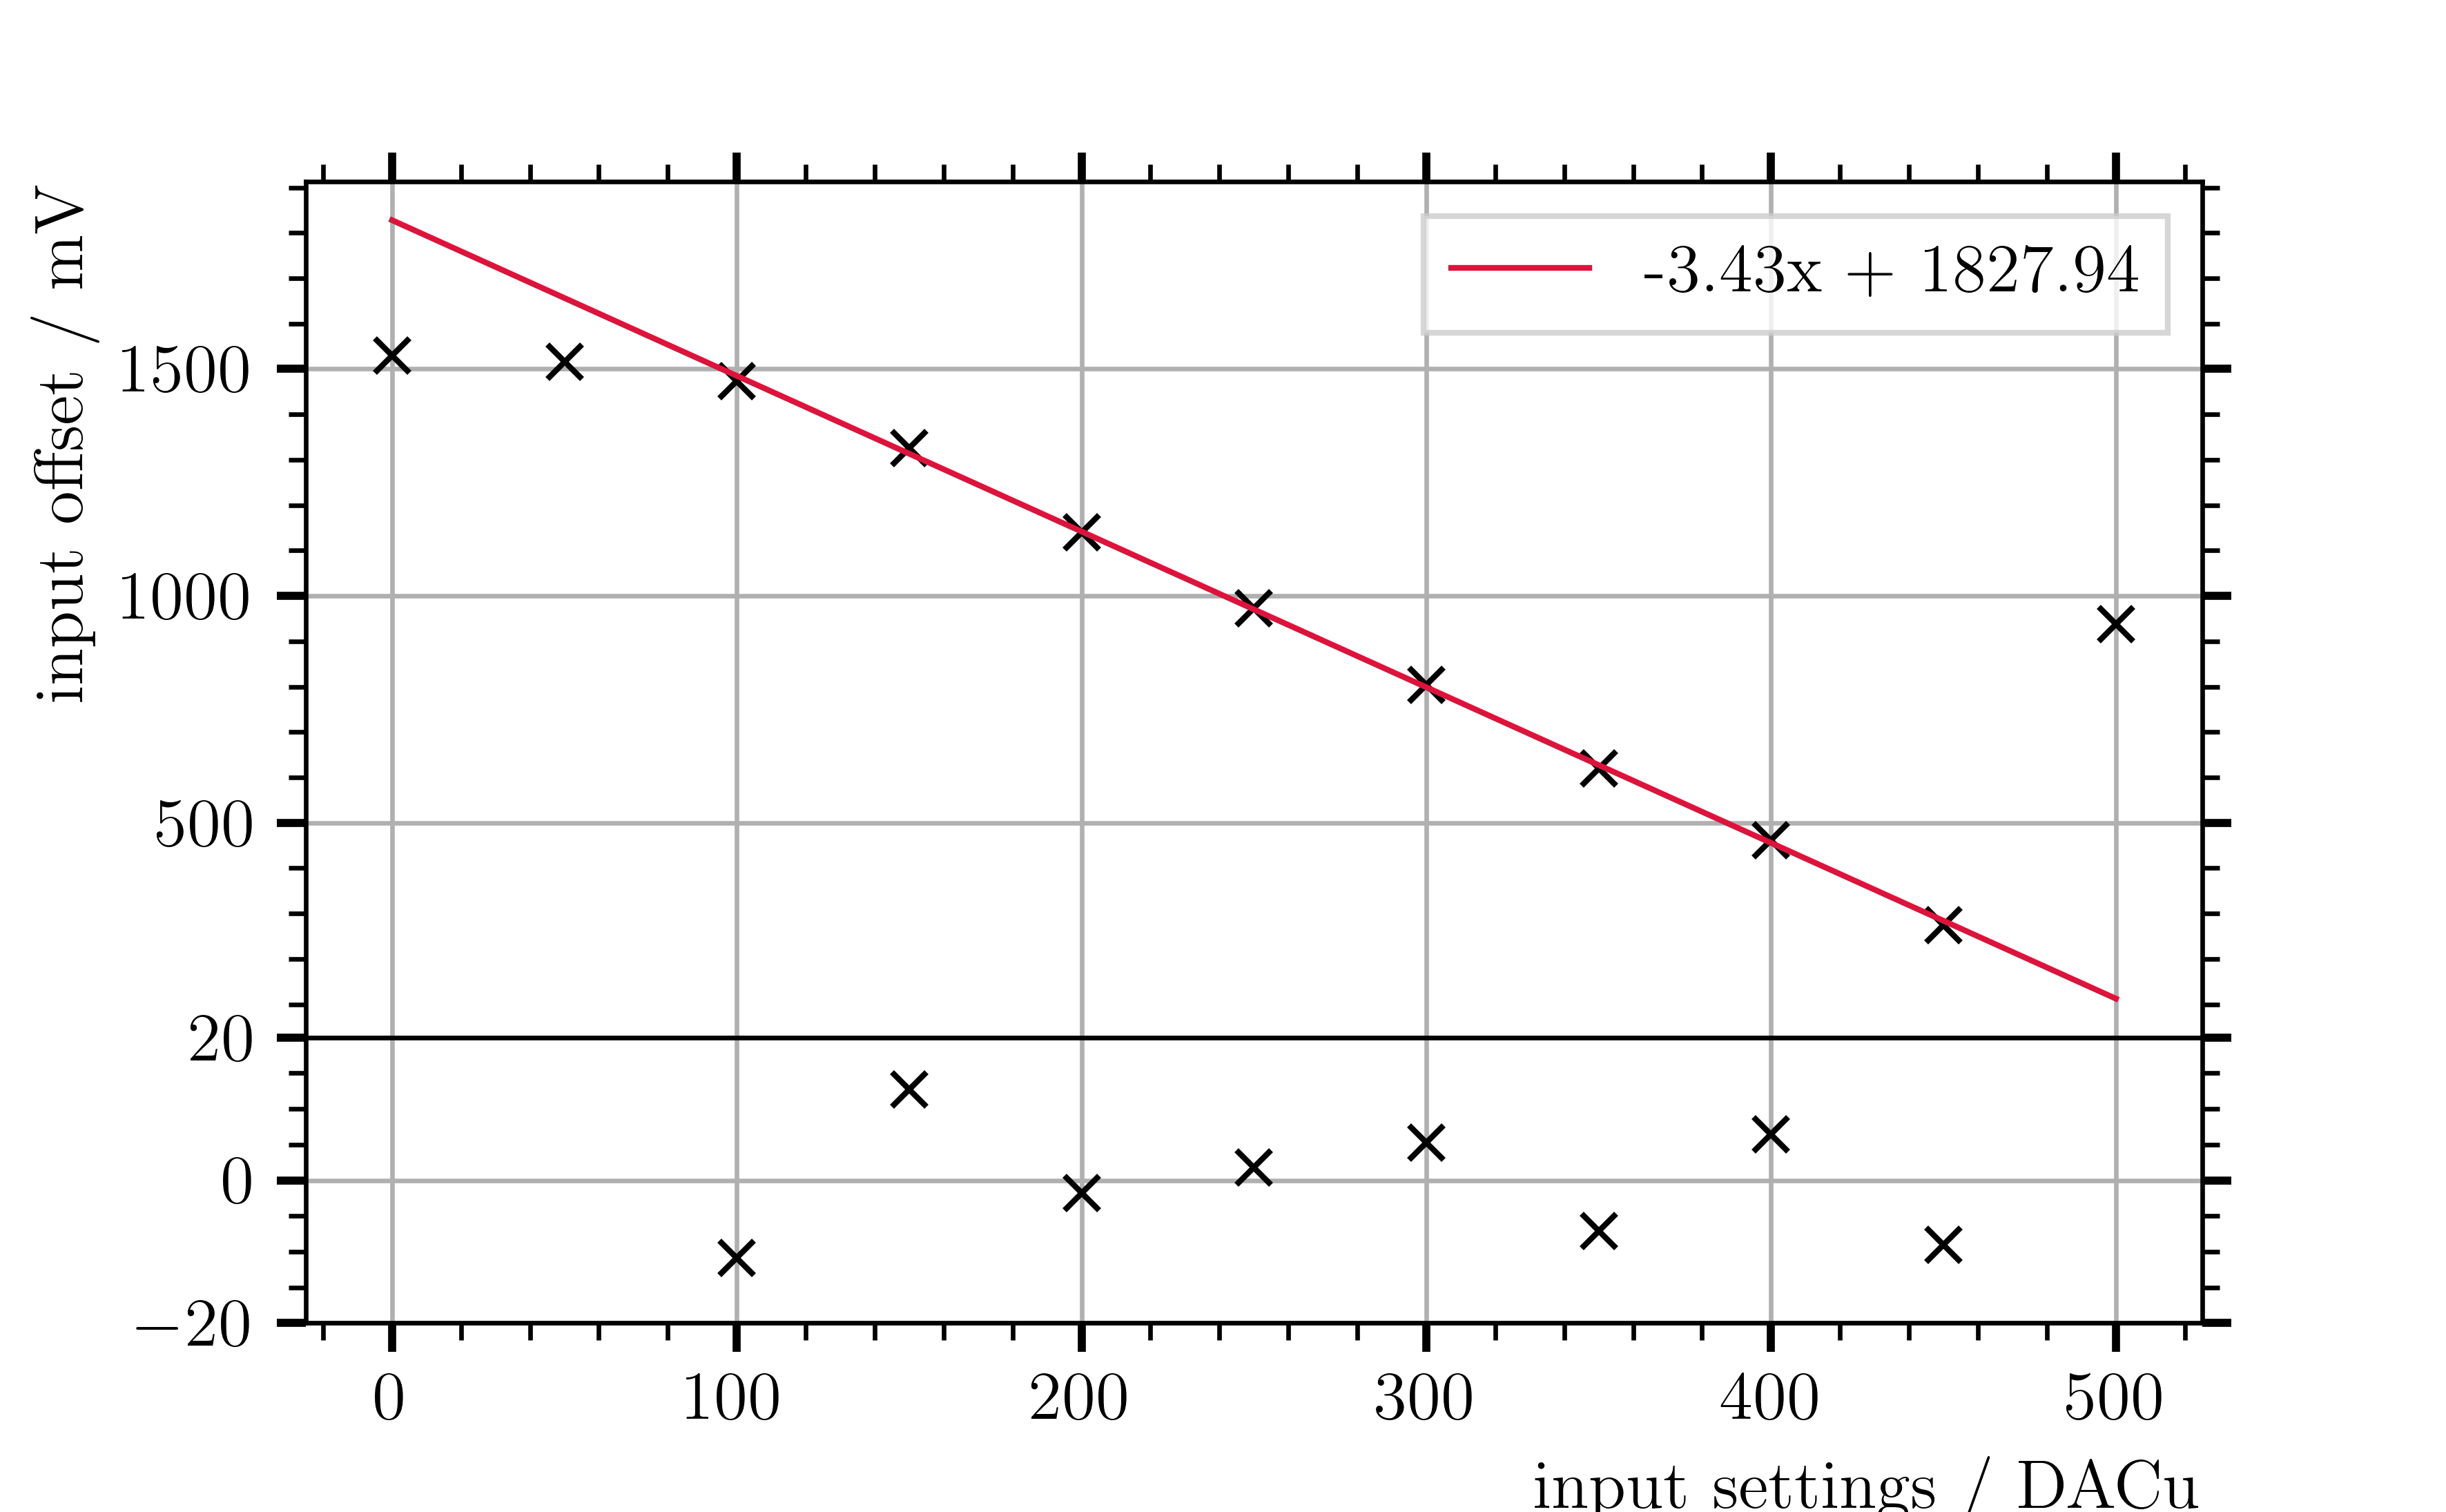
\includegraphics[width=.5\textwidth]{pictures/input_offset_board_2_channel_0.png}
		\caption{}
		\label{fig:input_offset_b2_dac50}
	\end{subfigure}
	\caption[todo]{todo}
	\label{fig:input_offset_b2_dac}
\end{figure}

After these measurements were done, for the \ac{emusic} boards 2 and 6 the settings for which all channels have \SI{1}{\volt} offset were determined.
The resulting \ac{dac} settings and the corresponding input voltages are listed in \autoref{tab:input_offset_equalized}.
With these settings the measurement of the pole-zero cancellation and the low and high trans-impedance and pole-zero attenuation were performed.
Which are presented in the following sections.
\begin{table}
	\centering
	\caption[todo]{todo}
	\label{tab:input_offset_equalized}
	\begin{tabular}{|c|c|c|c|}
	    \ac{emusic} board & channel & \ac{dac} settings / \si{\dacu} & input offset voltage / \si{\milli\volt} \\\hline
	\end{tabular}
\end{table}

\section{Pole-Zero Cancellation}

In this section pole-zero cancellation shaper and its effect with different settings tested.
The tests were done using the setup described in \autoref{sec:setup}.
For the amplification the \ac{emusic} board 2 was chosen and the digitization was done by a GANDALF module.
The \ac{emusic} settings of one of these measurements are shown in \autoref{} in the appendix.
For the other measurements, the only thing changing in the settings are the pole-zero settings.
Each measurement includes XXXXX events, for which the mean value is shown in the plots below.
The values for the amplitude and \ac{fwhm} were calculated for each individual waveform and theire mean values are presented here for the different measurements.

First the pole-zero cancellation was disabled to perform measurements for a reference amplitude and \ac{fwhm}.
In \autoref{fig:pz_no_pz} the mean of all waveforms, measured in channel 0, is shown.
The mean amplitude is 
\begin{align}
    V_{amp} &= \SI{1(1)}{\milli\volt}
\end{align}
and the \ac{fwhm} is
\begin{align}
    t_\text{FWHM} &= \SI{1(1)}{\nano\second}.
\end{align}

Next the measurement with enabled pole-zero cancellation and with fixed settings for its capacitor and variing resistor values.
The resistor settings were changed to all possible values, from 0 to 7, and the capacitor setting was kept at 31.
\autoref{fig:pz_resistor} presents the mean waveforms for the eight measurements.
The determined amplitudes and \ac{fwhm} and the coresponding decrease in respect to the values without pole-zero cancellation are listed in \autoref{tab:pz_resistor}.
Of all measurements the one with the resistor setting 0 had the highest mean amplitude with 
\begin{align}
    V_\text{amp,R=0} &= \SI{1(1)}{\milli\volt}
\end{align}
which correspondes to a amplitude attenuation of \SI{1(1)}{\percent}.
With these settings a \ac{fwhm} of
\begin{align}
    t_\text{FWHM,R=0} &= \SI{1(1)}{\nano\second}
\end{align}
was measured, which is \SI{1(1)}{\percent} of the \ac{fwhm} measured without pole-zero cancellation.
\begin{figure}
	\centering
	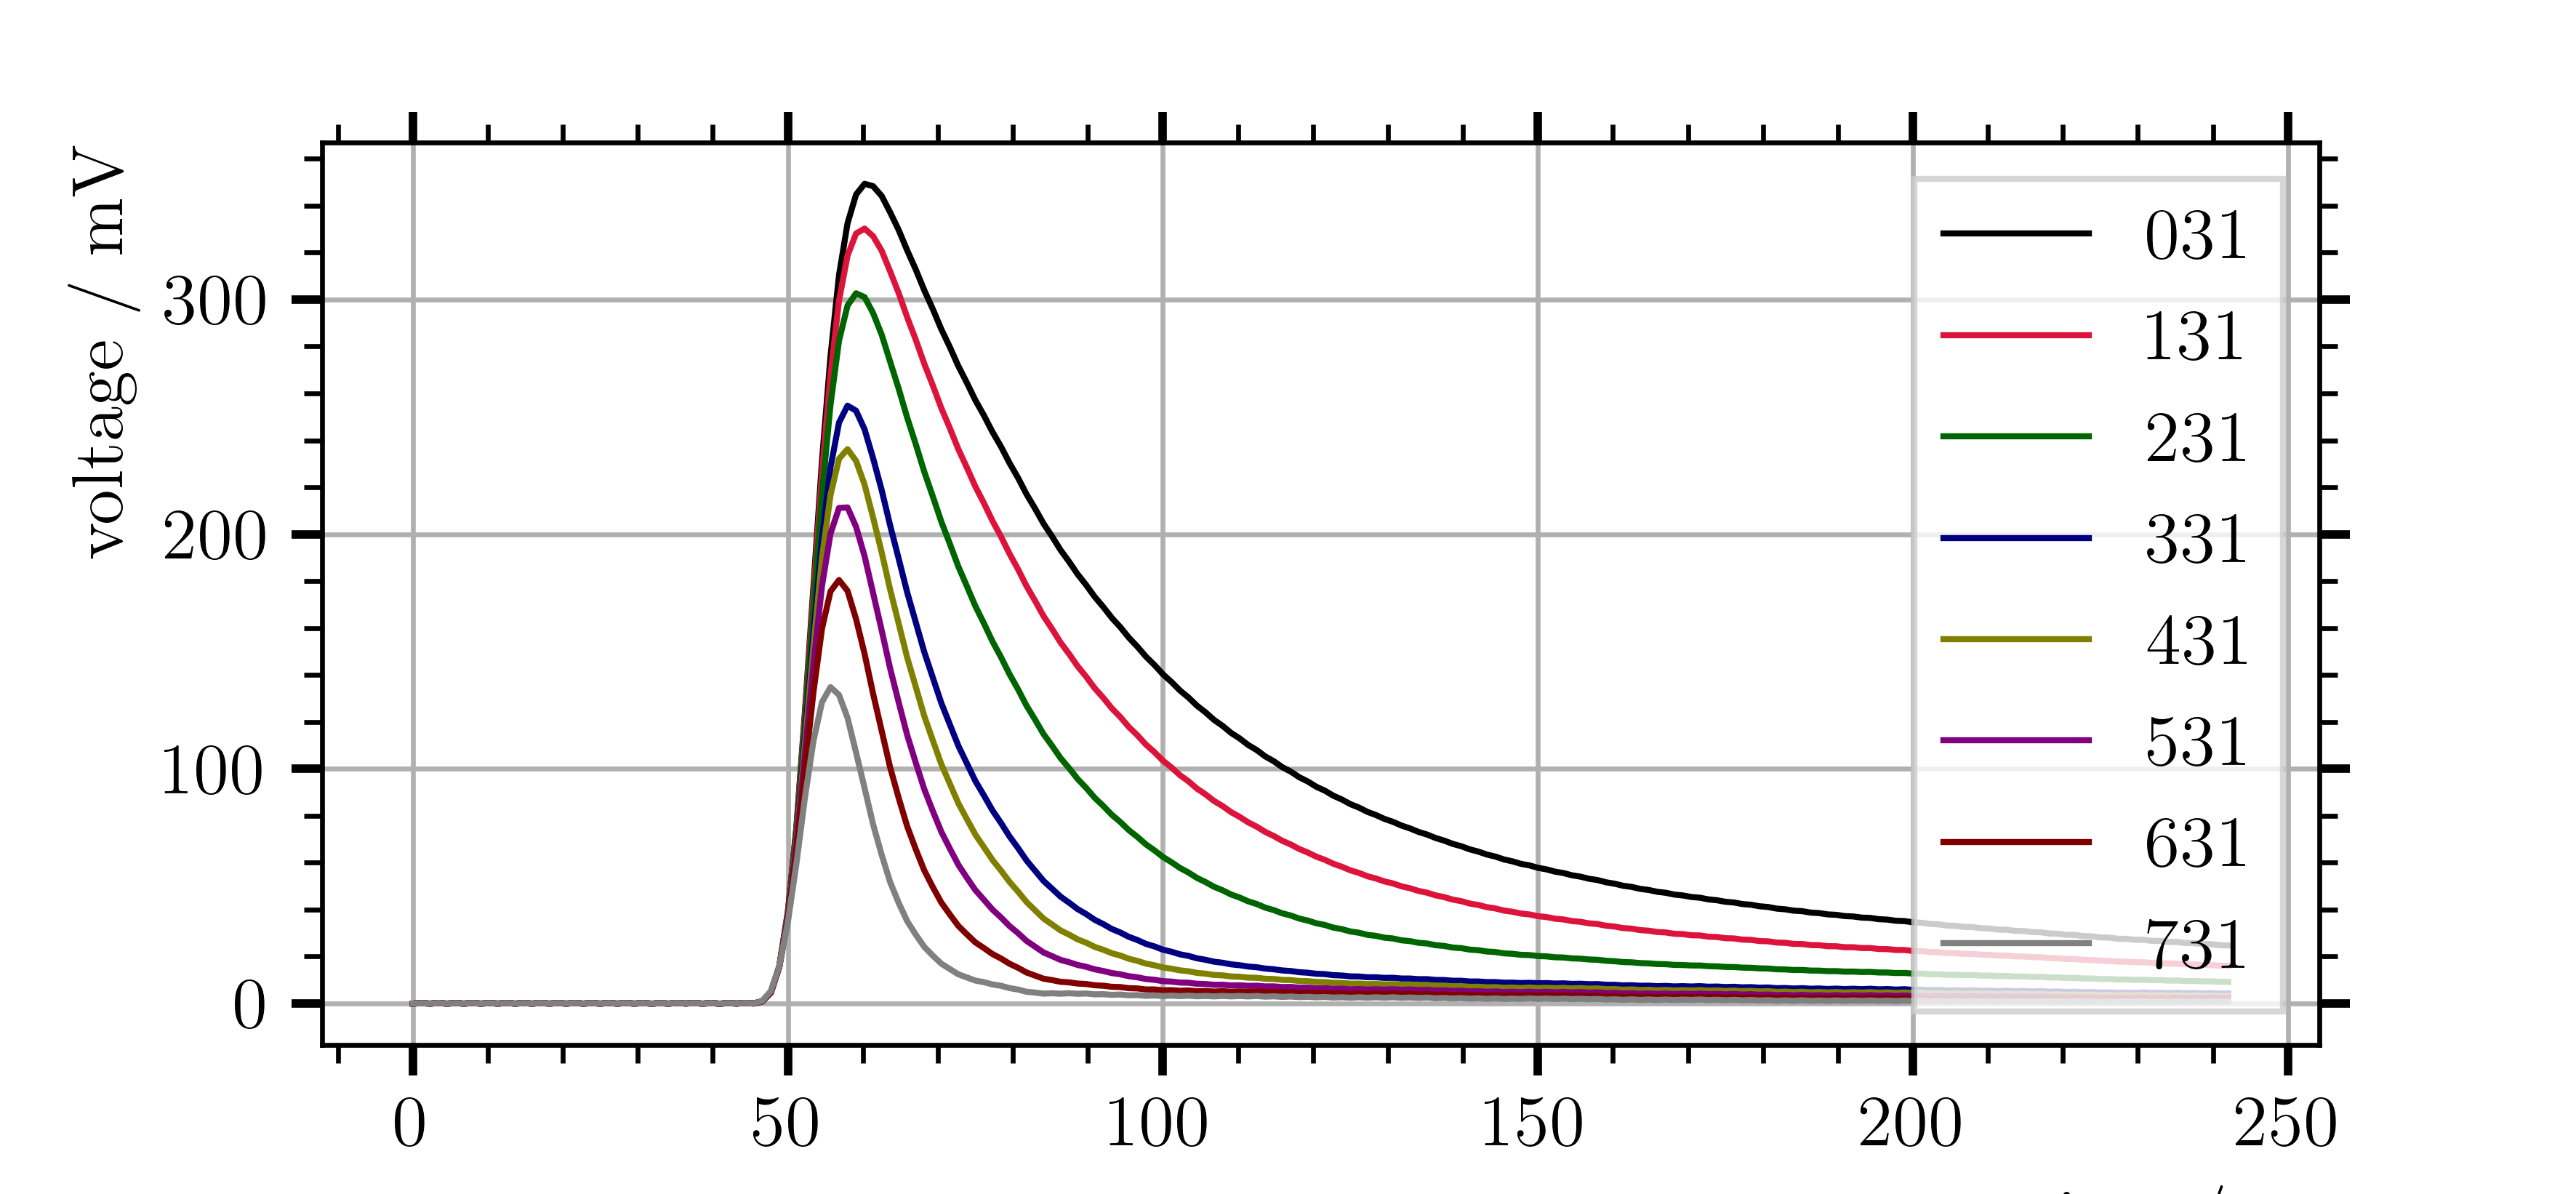
\includegraphics[width=1.\textwidth]{pictures/pz_resistor.png}
	\caption[Mean waveform for different pz-cancellation resistor values.]{Mean waveform for different pz-cancellation resistor values.}
	\label{fig:pz_resistor}
\end{figure}

The measurements with different capacitor settings were performed with the resistor setting of 0.
For the different measurements, the capacitor settings were changed to all 32 possible values, from 0 to 31.
In \autoref{tab:pz_capacitor} the mean values for the maximum amplitude and the \ac{fwhm} as well as the decrease compared to the values with disabled pole-zero cancellation are listed.
The mean waveforms for the measurements with the capacitor settings 0, 5, 10, 15, 20, 25, and 31 are shown in \autoref{fig:pz_capacitor}.
\begin{figure}
	\centering
	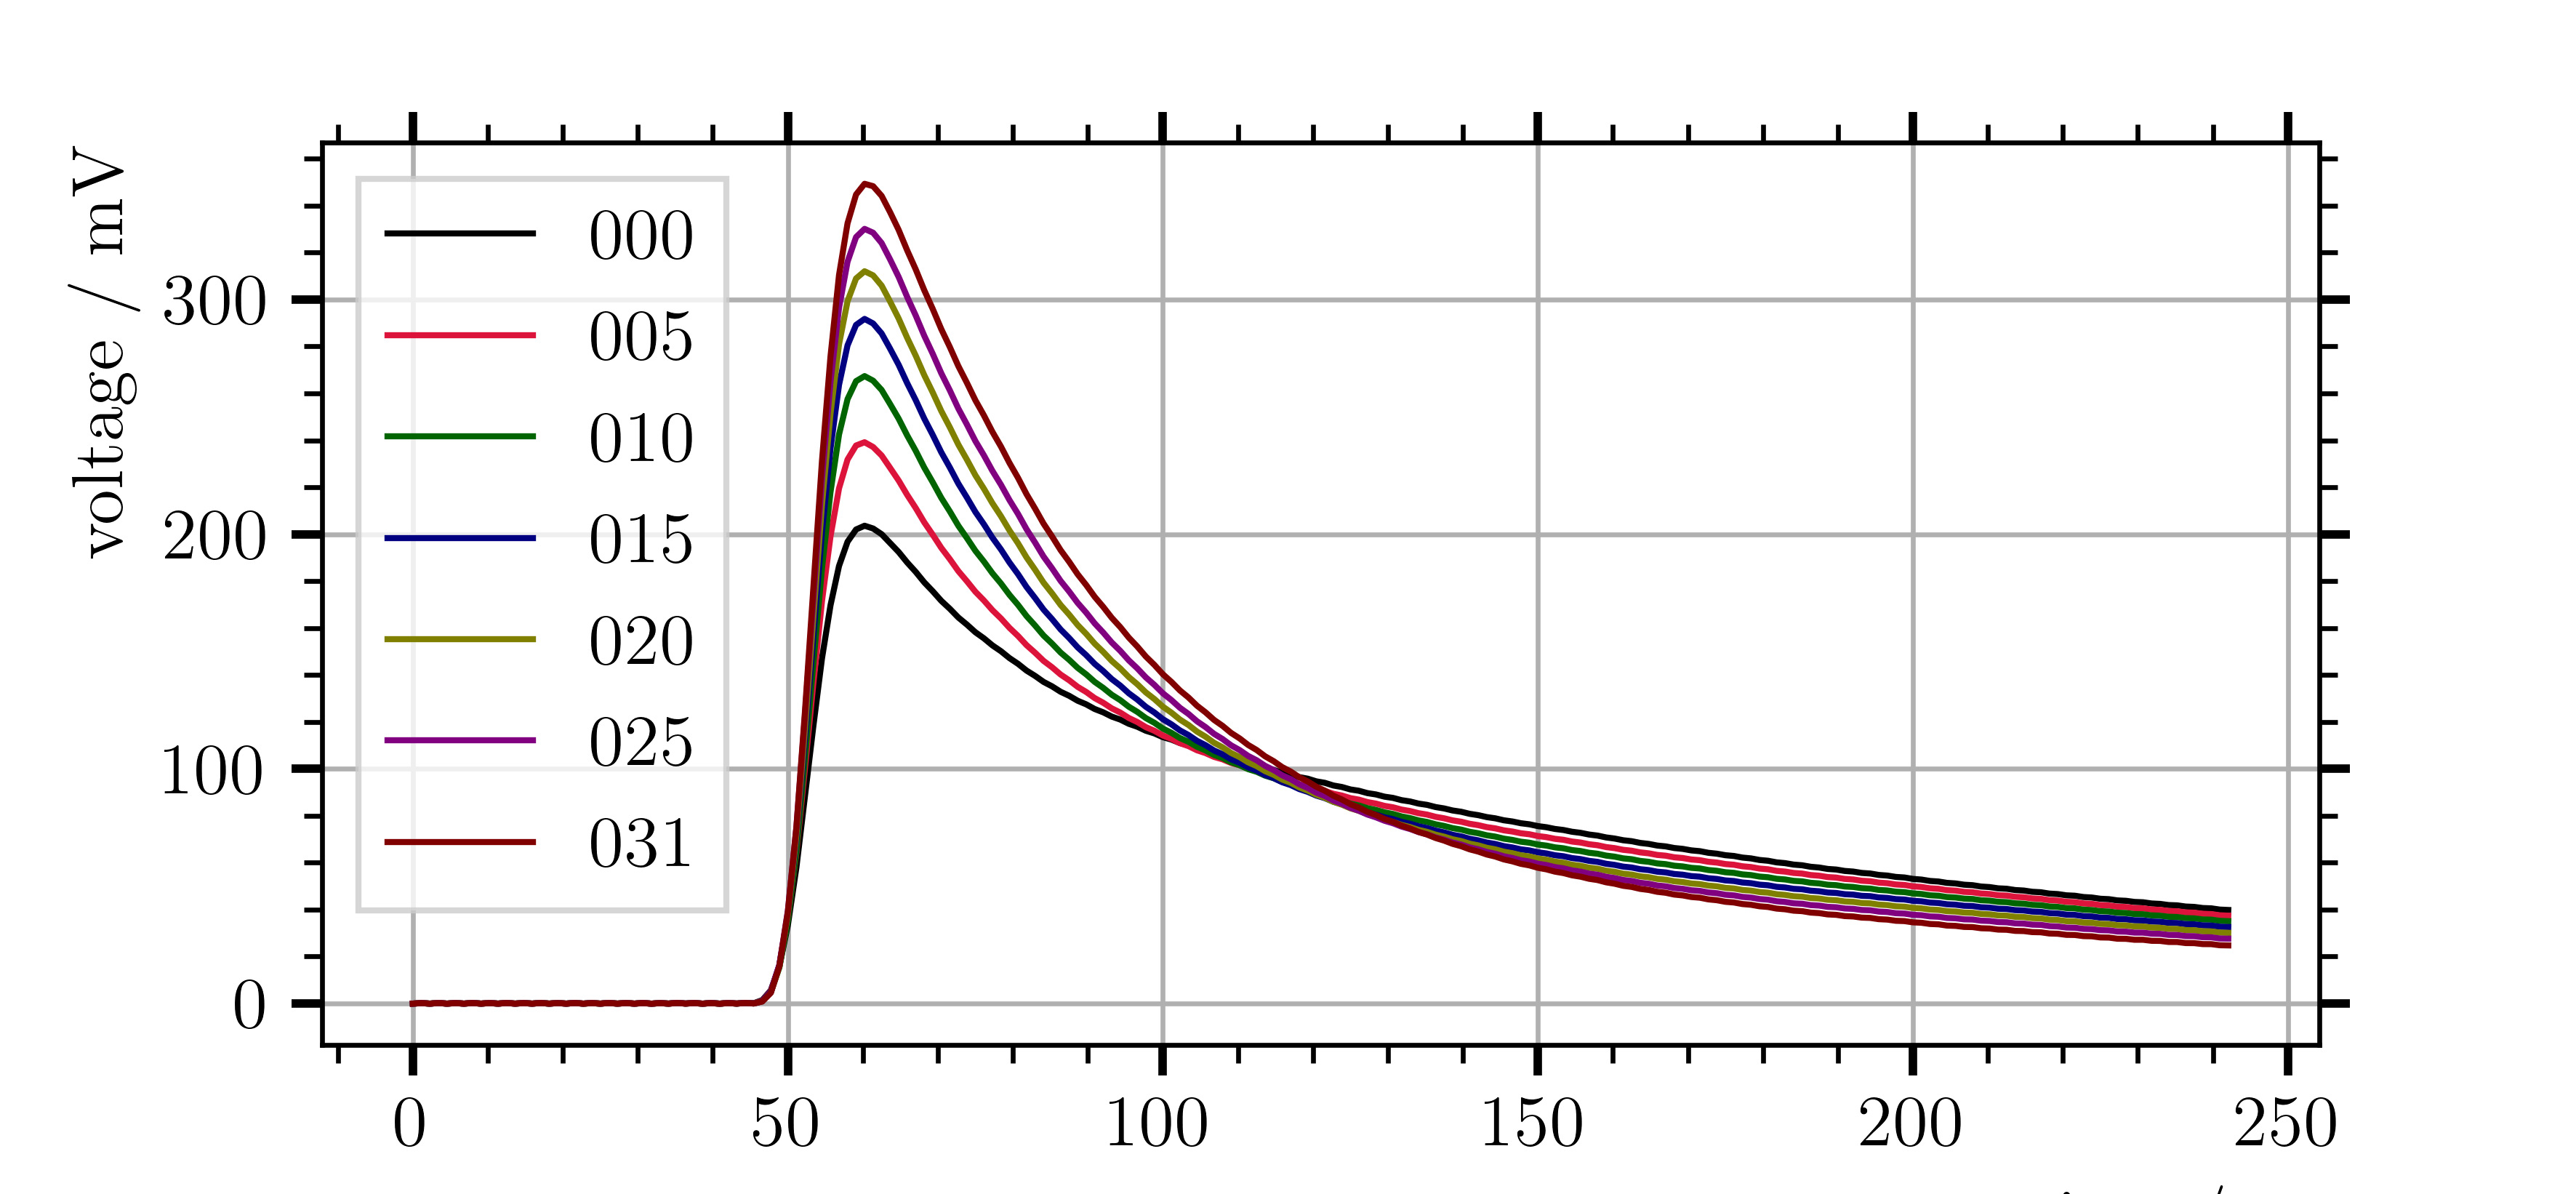
\includegraphics[width=1.\textwidth]{pictures/pz_capacitor.png}
	\caption[Mean waveform for different pz-cancellation capacitor values.]{Mean waveform for different pz-cancellation capacitor values.}
	\label{fig:pz_capacitor}
\end{figure}





\section{High and Low Transimpedance and Lower Attenuation}
After investigating the effects of the pole-zero shaper the influences between the normal and the low pole-zero attenuation settings are examined.
Also the high and low transimpedance settings are investigated.

First the pole-zero attenuation was looked at.
Therefore another meausrement without the lower attenuation setting was performed.
The pole-zero cancellation resistor setting was set to 3 and the capacitor setting was set to 31. 
In \autoref{fig:pz331_att} the mean waveforms with and without lower attenuation are presented.
The peak of the waveform is not affected by the lower attenuation setting.
Mainly the tail is of the waveform is increased in amplitude by using the lower attenuation.
This increases the peak width, but as it can be seen in \autoref{fig:pz331_att} it can also prevent small overshoot of the signal.

The measurement was also done with the pole-zero settings 7 and 0 for the resistor and capacitor, respectively.
The result is shown in \autoref{fig:pz700_att}.
Here the same behavior can be observed.
The peak amplitude is not influenced, only the amplitude of the tail is increased by the lower attenuation.
\begin{figure}
	\centering
	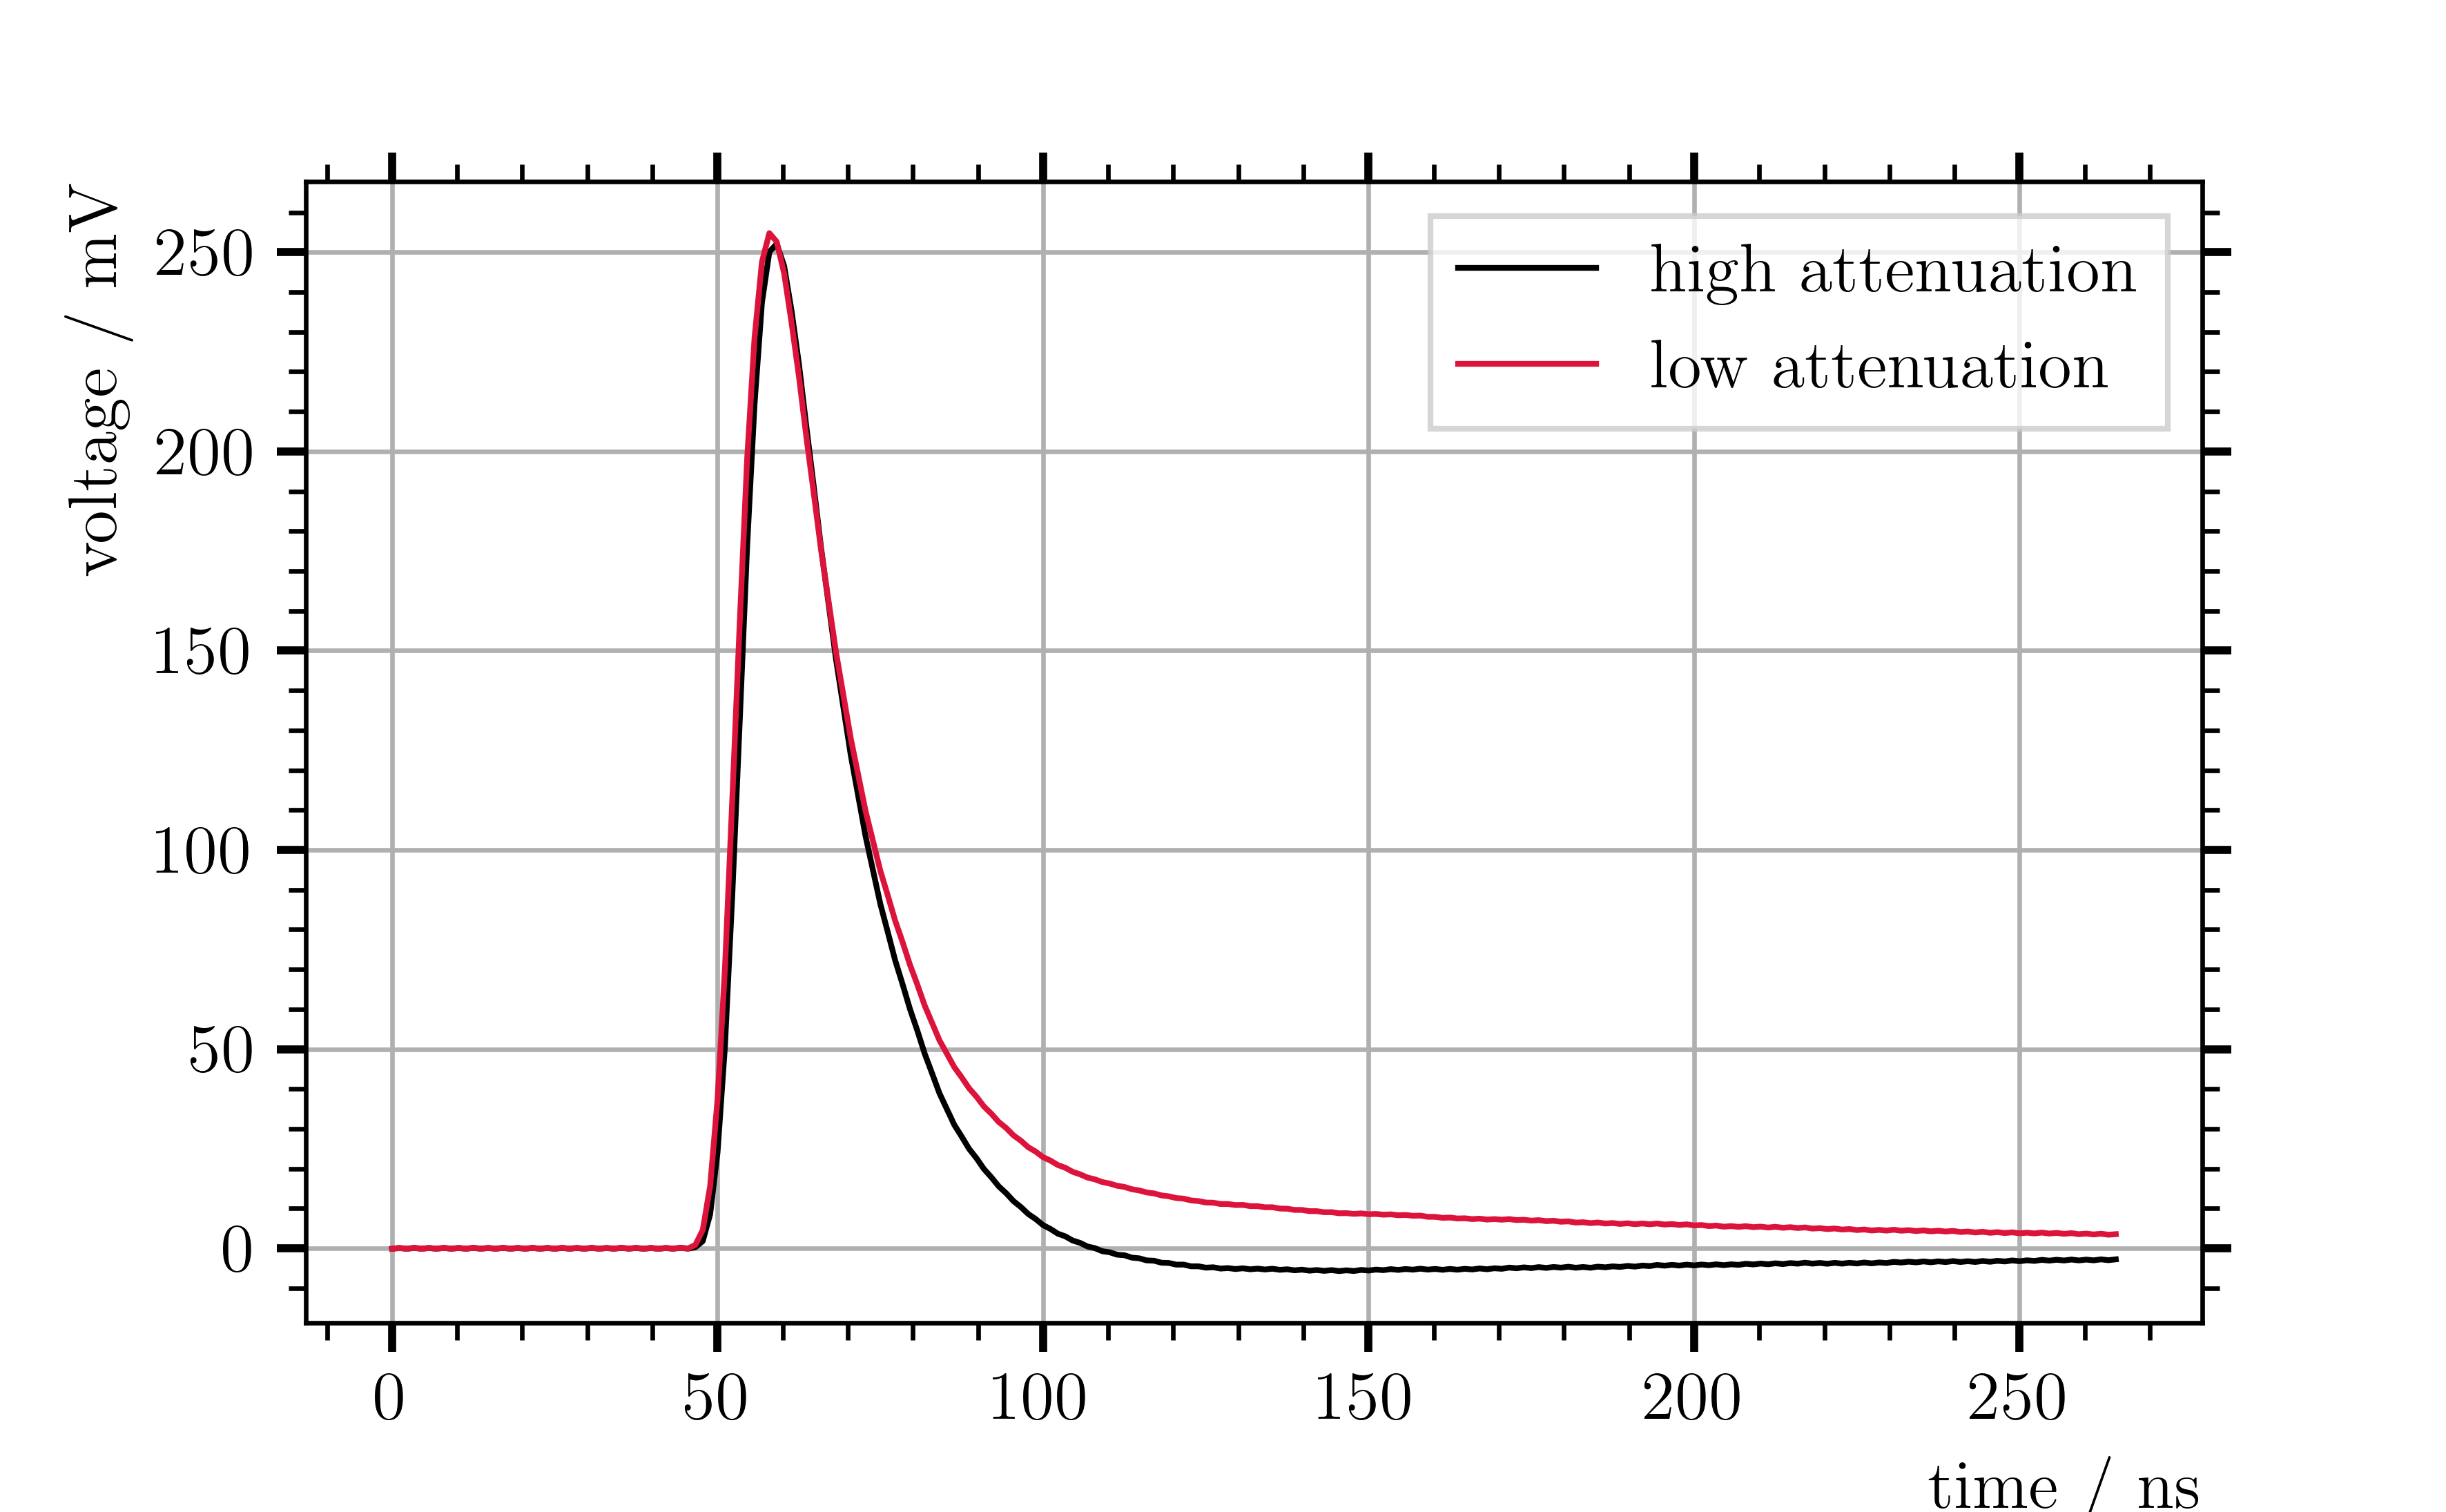
\includegraphics[width=1.\textwidth]{pictures/att_pz331}
	\caption[todo]{todo}
	\label{fig:pz331_att}
\end{figure}
\begin{figure}
	\centering
	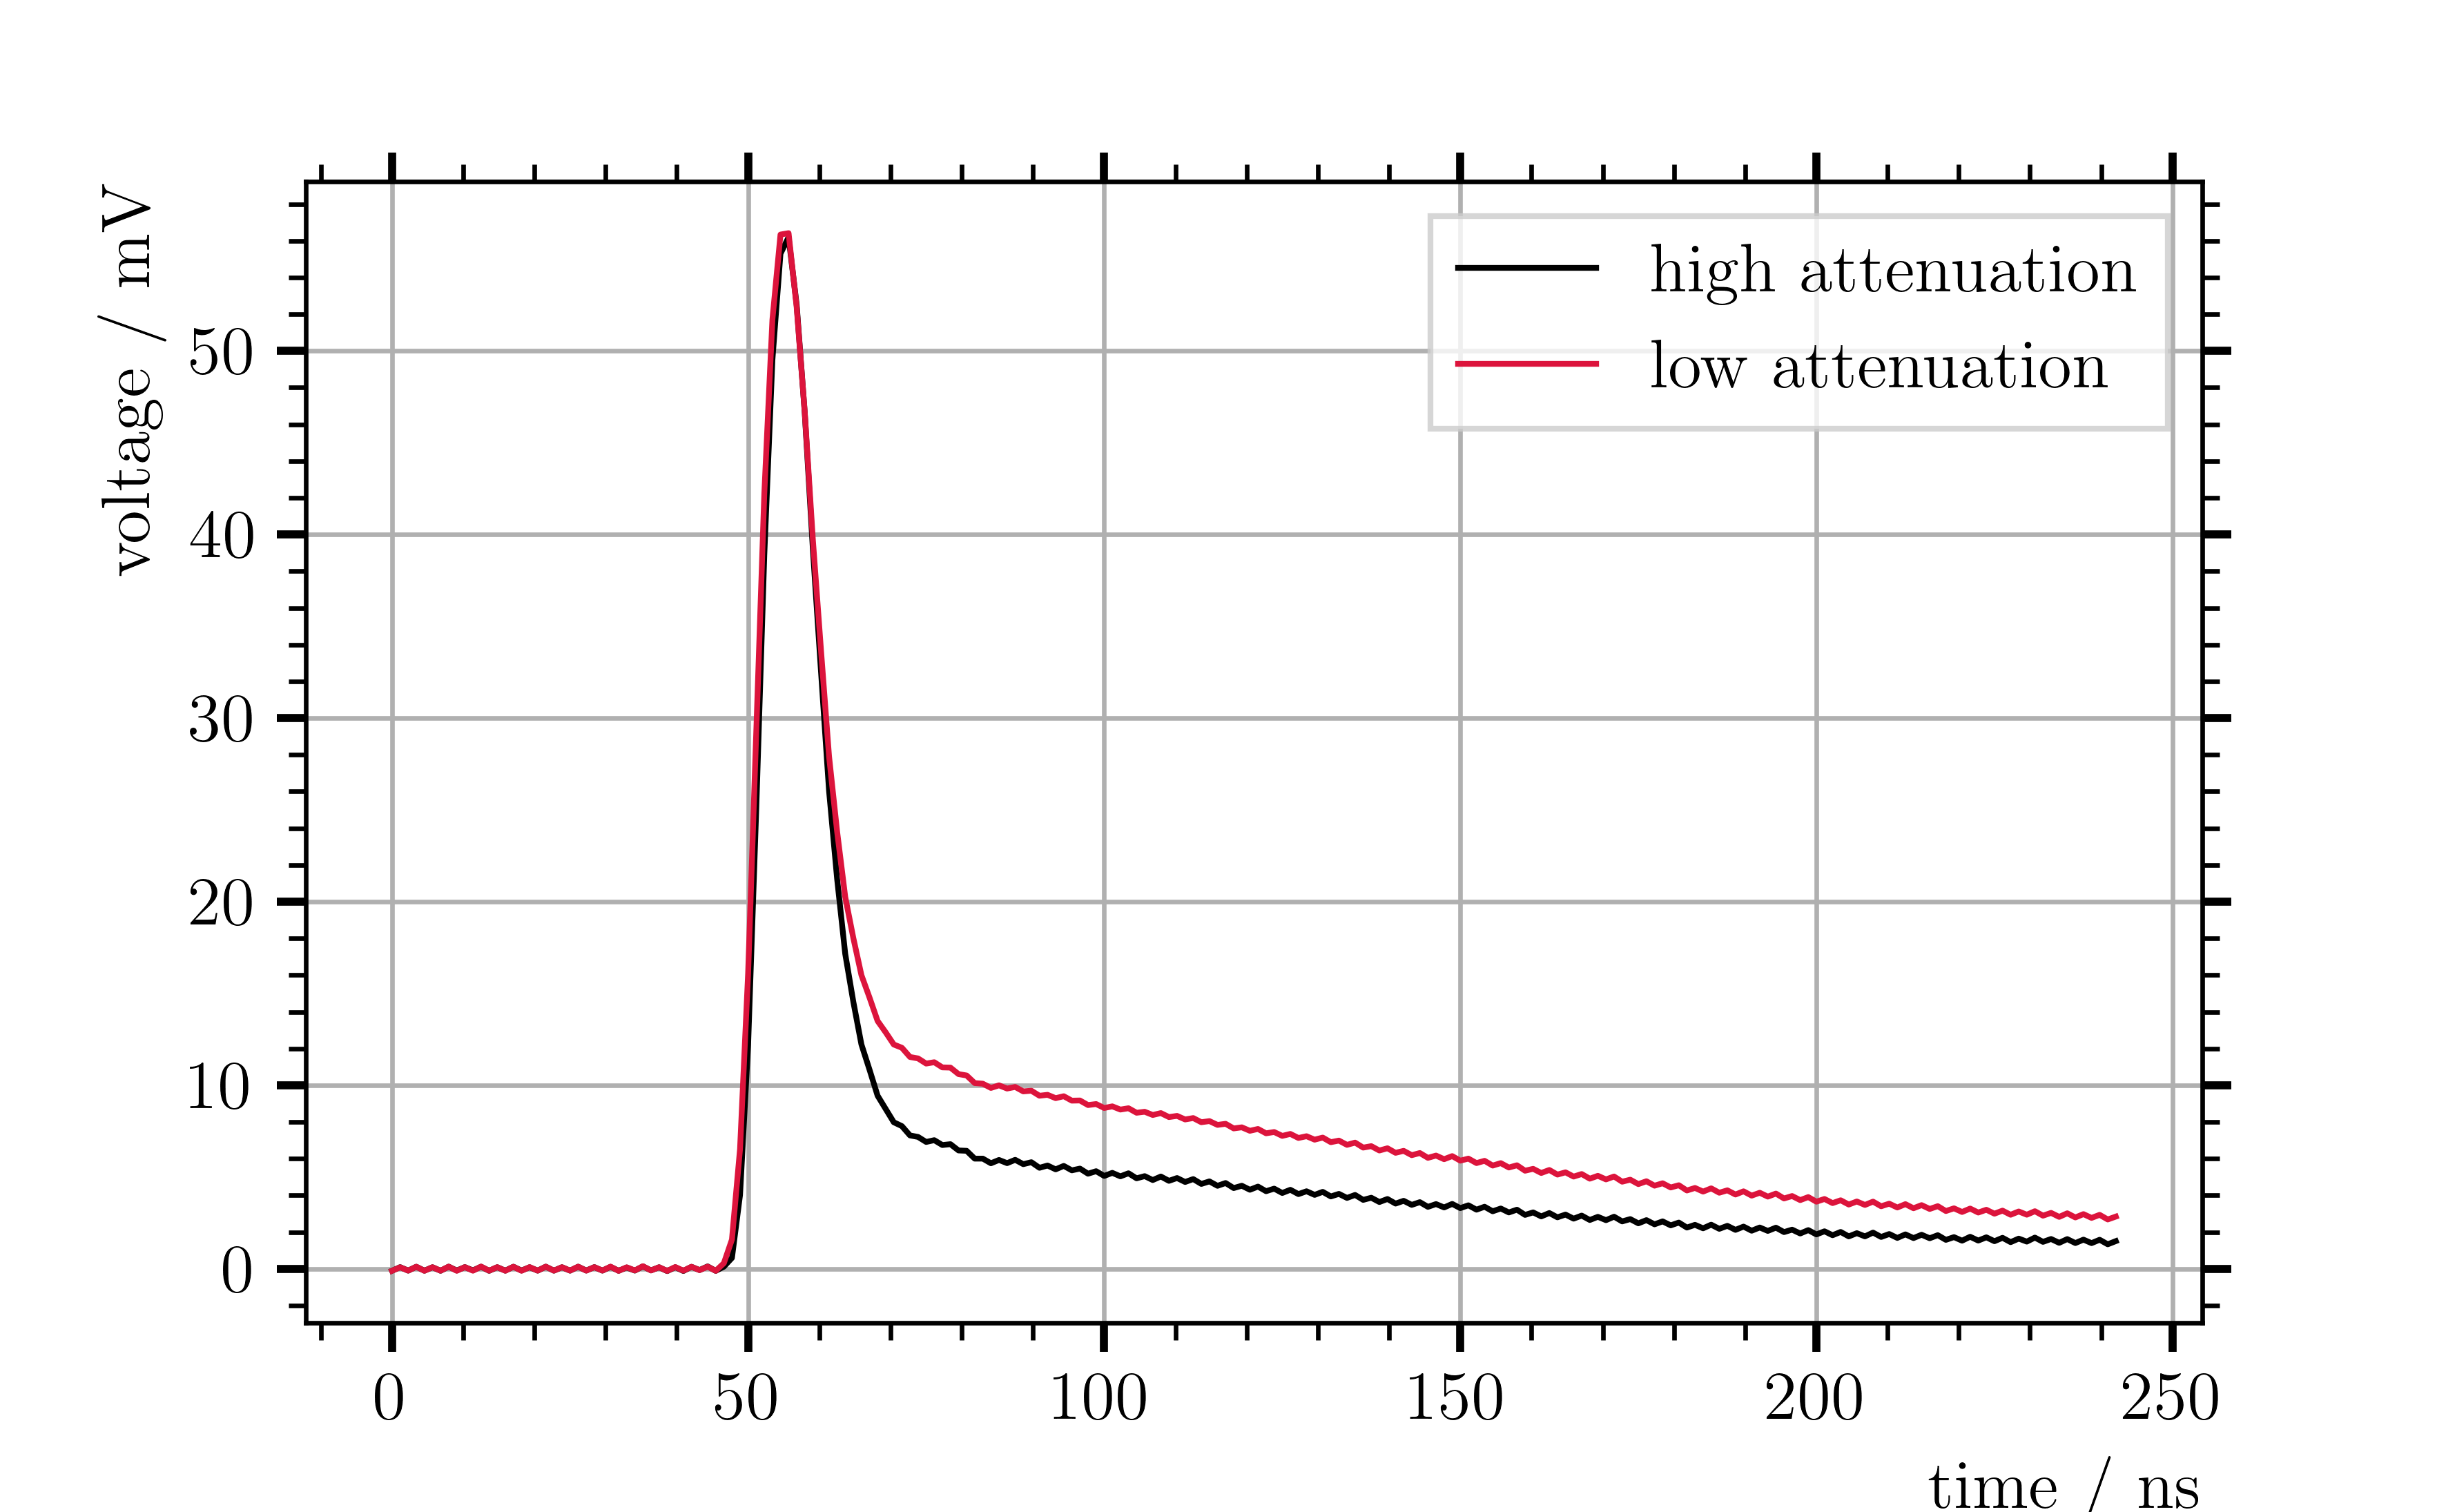
\includegraphics[width=1.\textwidth]{pictures/att_pz700}
	\caption[todo]{todo}
	\label{fig:pz700_att}
\end{figure}

After the pole-zero attenuation, the high and low transimpedance settings were investigated.
Therefore two measurements without pole-zero cancellation were taken with and without the high transimpedance.
Both measurements consist of around \num{30000} waveforms.
A mean waveform was calculated for both measurements and plotted in \autoref{fig:low_imp_wf}.
The mean amplitude of the events with high transimpedance is
\begin{align}
	V_\text{high imp} &= \SI{530(40)}{\milli\volt}
\end{align}
and of the events with low transimpedance the mean amplitude is
\begin{align}
	V_\text{low imp} &= \SI{175(13)}{\milli\volt}.
\end{align}
This results in a decrease by the factor \num{0.33(4)} if the low transimpedance is used.
Doing the same measurements using the pole-zero cancellation with both the resistor and capacitor settings set to 0 resulted in mean amplitudes of
\begin{align}
	V_\text{high imp} &= \SI{200(16)}{\milli\volt}\\
	\text{and}\quad V_\text{low imp} &= \SI{72(5)}{\milli\volt}
\end{align}
for high and low transimpedance respectively.
The signal amplitude decreases by the factor \num{0.36(4)}, which is in agreement with the value determined without pole-zero cancellation.
These measurements were repeated with the settings 3 and 31 for the pole-zero resistor and capacitor, respectively.
The mean amplitudes for these measurements are
\begin{align}
	V_\text{high imp} &= \SI{260(20)}{\milli\volt}\\
	\text{and}\quad V_\text{low imp} &= \SI{91(7)}{\milli\volt}
\end{align}
and the factor by which the signal amplitude decreases is \num{0.35(4)}, which is also in agreement with the results of the other two measurements.
The plots of the mean waveforms for the measurements with pole-zero cancellation are shown in the appendix in \autoref{} and \autoref{}.
\begin{figure}
	\centering
	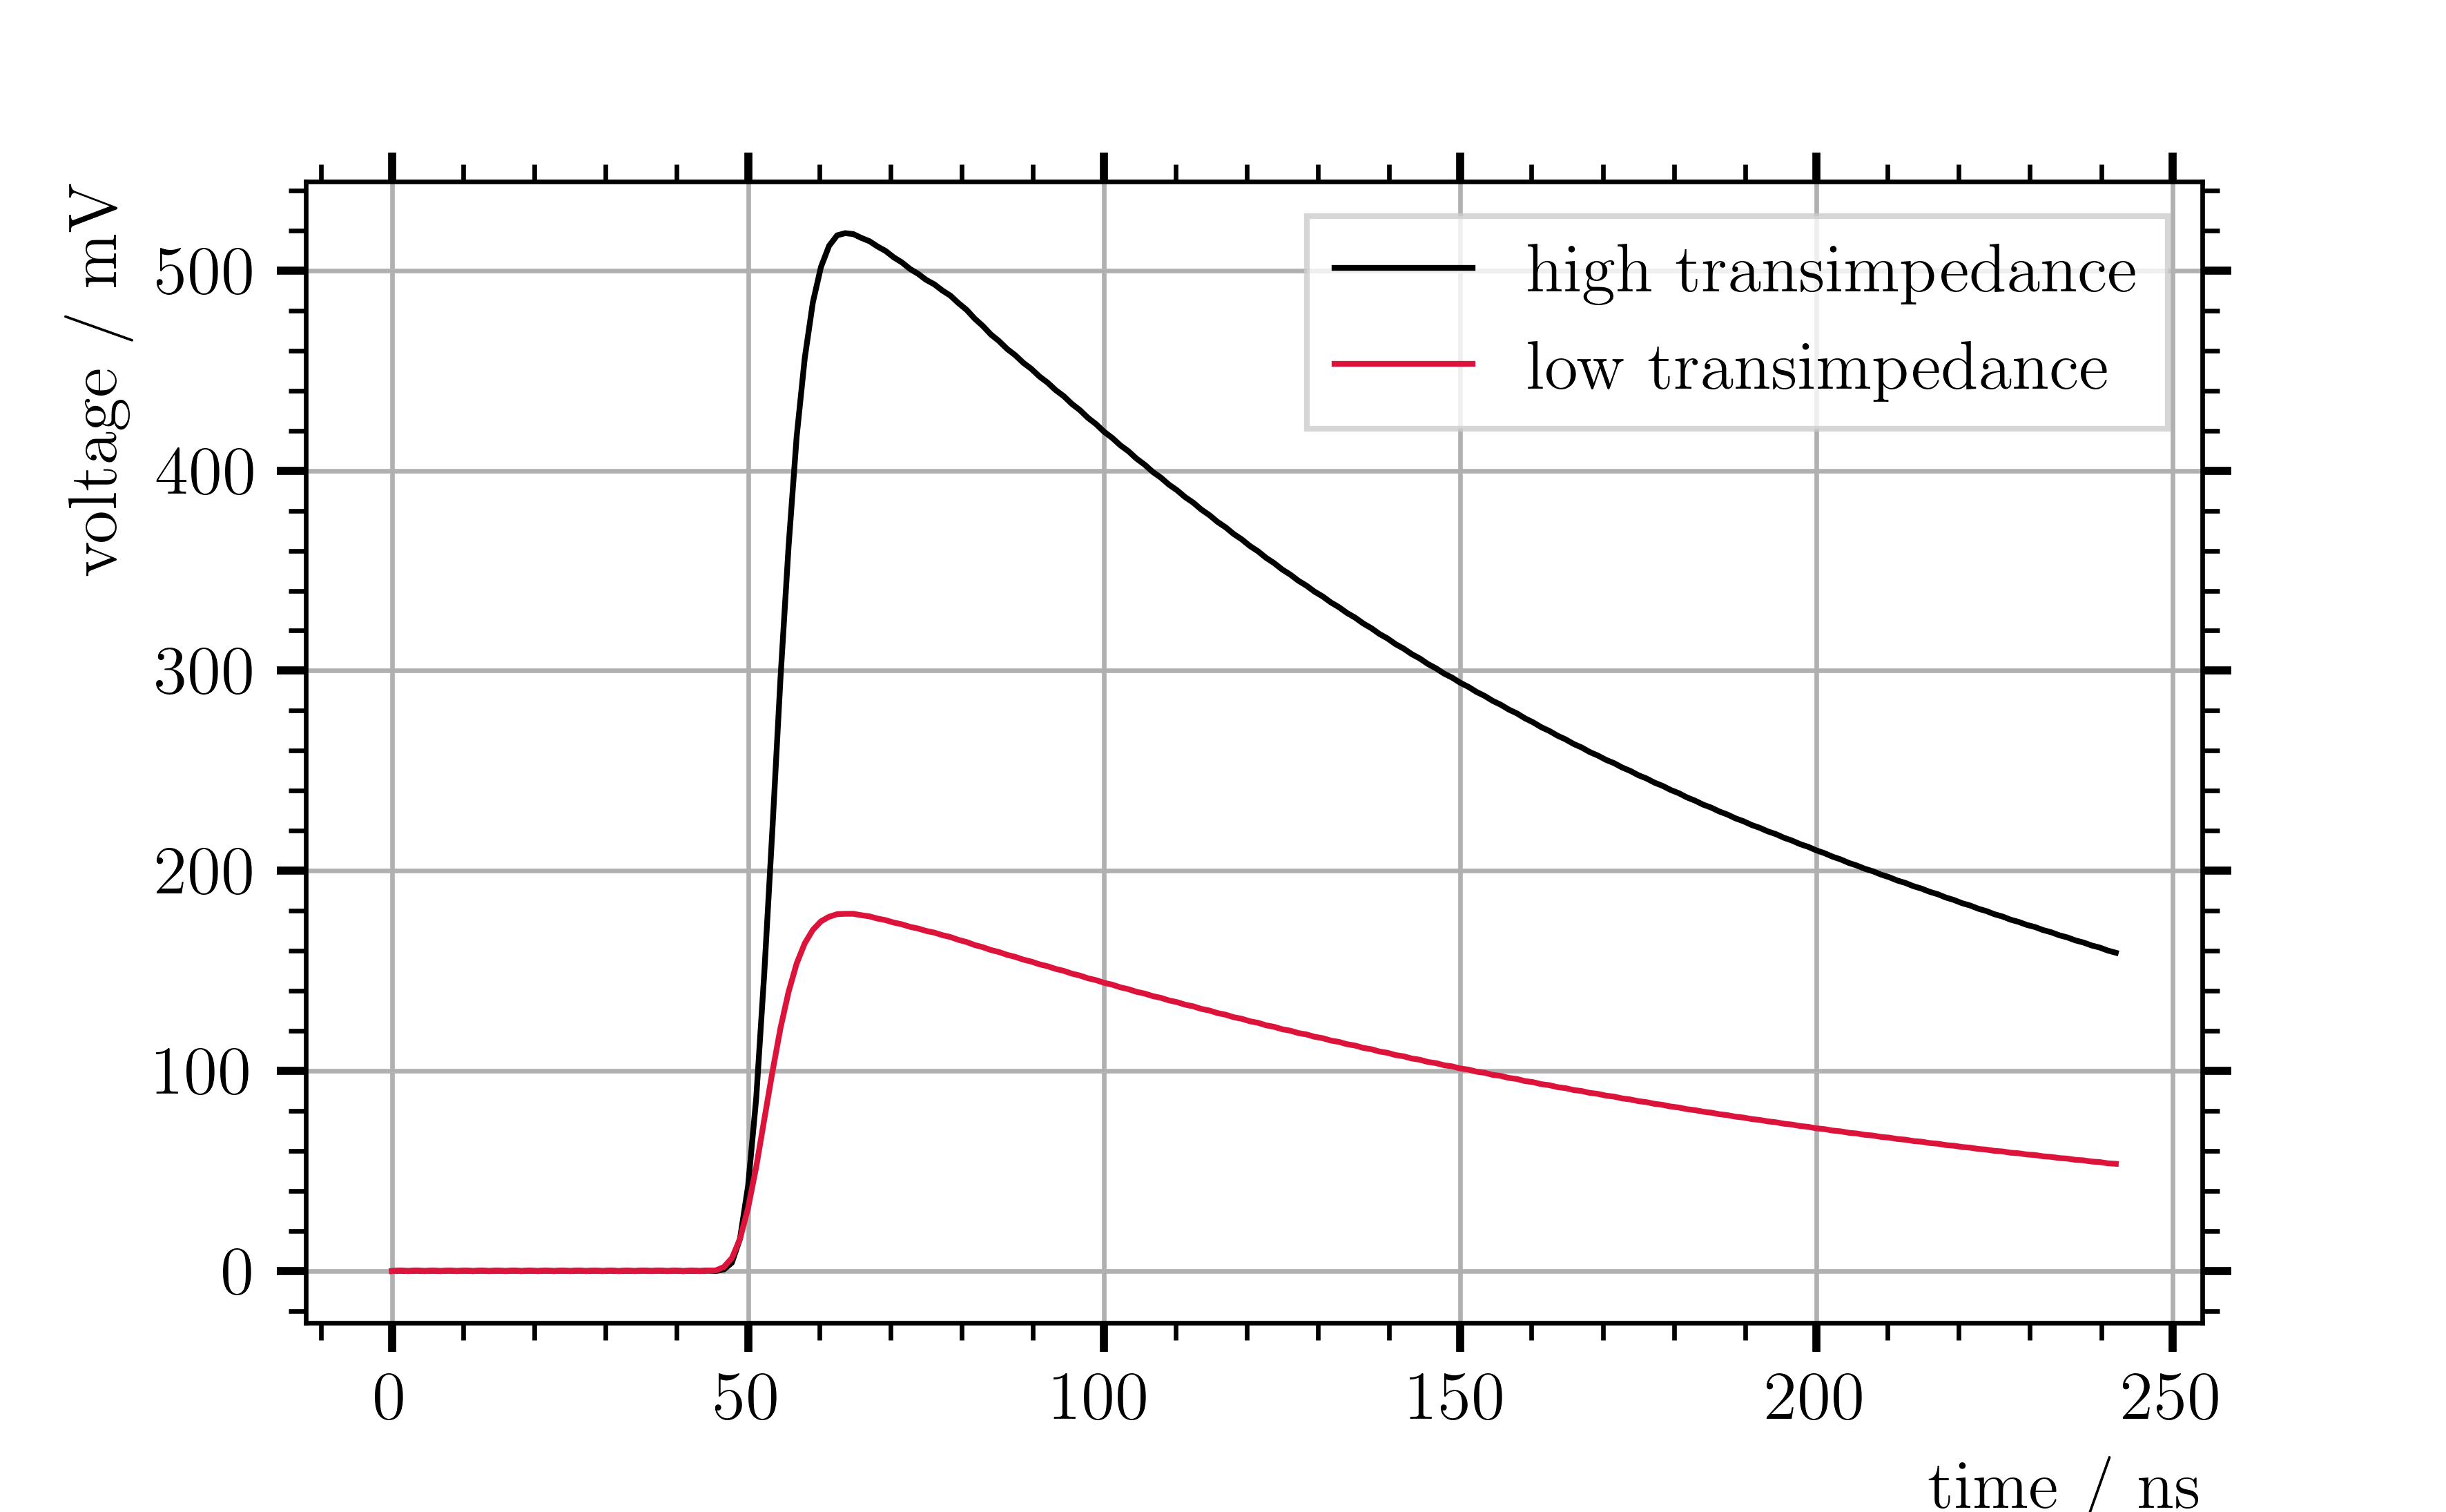
\includegraphics[width=1.\textwidth]{pictures/low_imp_mean_wf}
	\caption[todo]{todo}
	\label{fig:low_imp_wf}
\end{figure}

After the, for this work, most important features of the \ac{emusic} are investigated, a \ac{emusic} board and a Hamamatsu \ac{sipm} board were used to measure dark counts.
The goal of the dark count measurement was to test if dark counts could be used for calibration.

\section{Dark Count Measurements}


%\chapter{\ac{daq} performance at the \ac{desy} testbeam}
In october 2022 the One Cell Prototype was tested for one week at the \ac{desy} testbeam.
\autoref{fig:one_cell_testbeam} shows a picture of the the One Cell Prototype set up at the testbeam area.
The electron beam comes form the left, where it first passed a $2\times\SI{2}{\milli\meter\squared}$ square lead collimater.
Afterwards the electrons passed four plastic scintillators which are read out with \acp{pmt}.
A coincidence of the signals from all four \acp{pmt} is used to trigger the data aquisition.
After the scintitllators the One Cell Prototype is placed.
It stands on a rotary table to allow measurements with the beam coming from different angles, and on a \ac{desy} table, which enables left-right and up-down movement.
Measurements of each \num{10000} events were performed for XX positions by adjusting the position of the \ac{desy} table.
Each position was measured at different angles from \SIrange{0}{90}{\degree} in \SI{15}{\degree} steps by turning the detector on its rotary table.
For all positions and angles five measurements were done with variing beam energy starting from \SI{1.4}{\mega\electronvolt} up to \SI{5.4}{\mega\electronvolt} in \SI{1}{\mega\electronvolt} steps.






After the performance of the \ac{daq} was tested at the testbeam for one week with particles of known energy and known direction of movement, the long term performance of the one cell prototype and the \ac{daq} needs to be investigated.
For this purpose, the one cell prototype is assembled at the University of Freiburg, where it is supposed to be taking continuously data for a year.
Here the majority of events will be caused by cosmic muons.
By adding plastic scintillators with \acp{pmt} above and below the detector, trigger the data aquisition on a coincidence to only measure events, where the partice passed vertically through the detector.
Also a way to calibrate the detector needs to be found.

%\chapter{Summary and Outlook}
In this thesis a \ac{daq} for the readout of \acp{wom} was assembled and tested.
It consists of \ac{emusic} boards with \ac{emusic} chips for signal amplification and shaping and \ac{gandalf} moduls for digitization.
In the future it is supposed to be used for the long term test of the so called \qq{One Cell Prototype} in Freiburg.

A external clock was prepared for the \acp{gandalf} and tested for proper functionality.
This test was done by generating a pure \SI{150}{\mega\hertz} sine waveform with a arbitrary waveform generator and a narrow bandwidth \SI{150}{\mega\hertz} frequency filter.
The peak frequency of the digitized frequency was determined with a \ac{fft} is \SI{149.4(10)}{\mega\hertz} which is in agreement with the theoretical frequency of the sine waveform.
Therefore it can be concluded that the \acp{gandalf} sampling with the correct frequency of \SI{880}{\mega\sample\per\second} and the external clock is working as intended.
Also the \ac{gandalf} firmware was adjusted to trigger on positive input signals instead of negative pulses.
%Through a bug in the new firmware a surpassing of the maximum datarate of \SI{20}{\mega\byte\per\second} leads to incomplete events which cannot be decoded with the software of the \ac{gandalf}.
%This should not be a problem for the application with the One Cell Prototype since the datarate from firt tests is much lower than the limit.

The most important settings of the \ac{emusic} boards were tested.
The first of these was the measurement of the input offset voltage used to adjust the overvoltage of the \acp{sipm} on a channel by channel level.
It was found, that the input \ac{dac}, which sets the offset only follows a linear behavior between \SI{100}{\dacu} and \SI{450}{\dacu}.
In this range the linear behavior measured with the \ac{emusic} board 2 is XXX and for the \ac{emusic} board 6 it is XXX.
But the input offset differs between the different channels, therefore it is necessary to measure the input offset voltage while adjusting it.
For both boards the input \acp{dac} were set to get approximatly \SI{1}{\volt} input offset.


Also the pole-zero cancellation shaper was tested with different settings.
Therefore measurements with deactivated pole-zero cancellation shaper were made as a reference.
Also measurements with eight different settings for the shapers resistor at a constant setting for the shapers capacitor were done to see the effect of the resistor settings.
In order to see the effect of the capacitor eight measurements with different capacitor settings but the same resistor setting were performed.
The \ac{fwhm} of the signals could be reduced down to a minimum of \SI{}{\nano\second}, depending on the pole-zero cancellation settings.
But while the width decreased, the pole-zero cancellation shaper attenuated the signal amplitude down to \SI{}{}.
A \SI{}{\percent} reduction compared to the \SI{}{} amplitude without the pole-zero cancellation.
In addition to the different pole-zero settings, also the lower attenuation option of the pole-zero cancellation shaper and the high transimpedance mode was tested.

Two dark count measurements were performed, one with and one without the pole-zero cancellation shaper.
For the measurement with the pole-zero cancellation shaper, the resistor setting R=3 and the capacitor setting C=31 were chosen.
In the histogram of the waveform integrals of both measurements no single photoelectron peaks could be distinguished.
Hence it was not possible to use dark count measurements for calibration.

The \ac{emusic} board was succesfully tested at the \ac{desy} testbeam and will be under a long time performens test starting in the near future.


\appendix

\chapter{List of acronyms}
\begin{acronym}[SiPM]
    \acro{sm}[SM]{Standard Model}
    \acro{lhc}[LHC]{Large Hadron Colider}
    \acro{ship}[SHiP]{Search for Hidden Particles}
    \acro{sps}[SPS]{Super Proton Synchrotron}
    \acro{sbt}[SBT]{Surrounding Background Tagger}
    \acro{sipm}[SiPM]{Silicon Photomultiplier}
    \acro{pcb}[PCB]{Printed Circuit Board}
    \acro{asic}[ASIC]{Application Specific Integrated Circuit}
    \acro{dac}[DAC]{Digital to Analog Converter}
    \acro{adc}[ADC]{Analog to Digital Converter}
    \acro{apd}[APD]{Avalanche Photodiode}
    \acro{daq}[DAQ]{Data Acquisition}
    \acro{wom}[WOM]{Wavelengthshifting Optical Module}
    \acro{spad}[SPAD]{Single Photon Avalanche Diode}
    \acro{dc}[DC]{Dark Count}
    \acro{dcr}[DCR]{Dark Count Rate}
    \acro{fpga}[FPGA]{Field Programmable Gate Array}
    \acro{desy}[DESY]{Deutsches Electronen SYnchrotron}
    \acro{emusic}[eMUSIC]{enhanced Multiple Use SiPM IC for photodetector readout}
    \acro{pmt}[PMT]{Photomultiplier tube}
    \acro{amc}[AMC]{Analoge Mezzanine Card}
    \acro{omc}[OMC]{Optical Mezzanine Card}
    \acro{dmc}[DMC]{Digital Mezzanine Card}
    \acro{nim}[NIM]{Nuclear Instrumentation Module}
    \acro{hs}[HS]{Hidden Sector}
    \acro{lab}[LAB]{Linear Alkyl Benzene}
    \acro{fwhm}[FWHM]{Full Width at Half Maximum}
    \acro{compass}[COMPASS]{Common Muon Proton Apparatus for Structure and Spectroscopy}
    \acro{enob}[ENOB]{Effective Number of Bits}
    \acro{ppo}[PPO]{Diphenyloxazole}
\end{acronym}


\newpage
\listoffigures

\newpage

\listoftables
\newpage

\begin{thebibliography}{9}
\bibitem{ship} SHiP - Search for Hidden Particles, \url{https://ship.web.cern.ch/}, June 2022
\bibitem{ship_facility} S. Alekhin et al ``A facility to search for hidden particles at the CERN SPS: the SHiP physics case'', Rep. Prog. Phys. 79, Oct 2016, \url{https://doi.org/10.1088/0034-4885/79/12/124201}
\bibitem{ship_coll} SHiP Collaboration, ``SPS Beam Dump Facility - Comprehensive Design Study'', 2020, arXiv:1912.06356
\bibitem{kemp} J. Kemp, ``Development of a silicon photomultiplier based scintillator detector for cosmic air showers'' Phd thesis, Dez 2020, RWTH Aachen
\bibitem{nucl} F. Acerbi, S. Gundacker, ``Understanding and simulating SiPMs'', NIM-A vol. 926, p. 16-35, 2019. doi: 10.1016/j.nima.2018.11.118
\bibitem{HAMA_mppc} Hamamatsu Photonics, MPPC, \url{https://www.hamamatsu.com/content/dam/hamamatsu-photonics/sites/documents/99_SALES_LIBRARY/ssd/mppc_kapd9005e.pdf}, date: 20.06.2022
\bibitem{HAMsipm_ds} Hamamatsu S14160-3050HS Datasheet,
\url{https://www.hamamatsu.com/content/dam/hamamatsu-photonics/sites/documents/99_SALES_LIBRARY/ssd/s14160_s14161_series_kapd1064e.pdf}, date: 05.05.2022
\end{thebibliography}




\end{document}
